\documentclass[]{report}
\usepackage[a4paper, total={7in, 9in}]{geometry}
\usepackage[italian]{babel}
\usepackage[T1]{fontenc}
\usepackage[utf8]{inputenc}
\usepackage{float}
\usepackage{titlepic}
\usepackage{amsmath}
\usepackage{amssymb}
\usepackage{mathtools}
\usepackage{eucal}
\DeclareMathAlphabet{\mathpzc}{OMS}{cmsy}{m}{n}
\usepackage{graphicx}
\usepackage{rotating}
\usepackage[caption = false]{subfig}
\usepackage{caption}
\captionsetup{justification=justified,singlelinecheck=on, format=hang} % format=hang
\usepackage{color}
\usepackage{enumitem}
\usepackage[hang,flushmargin]{footmisc}
\usepackage{comment}
\usepackage{hyperref}
\hypersetup{
	bookmarks=true,         % show bookmarks bar?
	unicode=false,          % non-Latin characters in Acrobat’s bookmarks
	pdftoolbar=true,        % show Acrobat’s toolbar?
	pdfmenubar=true,        % show Acrobat’s menu?
	pdffitwindow=false,     % window fit to page when opened
	pdfstartview={FitH},    % fits the width of the page to the window
	pdftitle={Esercizi Analisi Statistica dei Dati 2016/2017},    % title
	pdfauthor={Gabriele Bellomia},     % author
	pdfsubject={Laurea Magistrale in Fisica},   % subject of the document
	pdfcreator={PdfLaTeX},   % creator of the document
	pdfproducer={TeXstudio}, % producer of the document
	pdfkeywords={keyword1, key2, key3}, % list of keywords
	pdfnewwindow=true,      % links in new PDF window
	colorlinks=true,       % false: boxed links; true: colored links
	linkcolor=black,          % color of internal links (change box color with linkbordercolor)
	citecolor=green,        % color of links to bibliography
	filecolor=magenta,      % color of file links
	urlcolor=blue           % color of external links
}

\usepackage{listings}

\definecolor{codegreen}{rgb}{0,0.6,0}
\definecolor{codegray}{rgb}{0.5,0.5,0.5}
\definecolor{codeblue}{rgb}{0.3,0.5,0.9}
\definecolor{codeorange}{rgb}{0.5,0.2,0}
\definecolor{backcolour}{rgb}{0.97,0.97,0.97}

\lstdefinestyle{Rstyle}{
	backgroundcolor=\color{backcolour},   
	commentstyle=\color{codegreen},
	keywordstyle=\color{codeblue},
	numberstyle=\tiny\color{codegray},
	stringstyle=\color{codeblue},
	basicstyle=\ttfamily\small,
	breakatwhitespace=false,         
	breaklines=true,                 
	captionpos=b,                    
	keepspaces=true,                 
	numbers=left,                    
	numbersep=5pt,                  
	showspaces=false,                
	showstringspaces=false,
	showtabs=false,                  
	tabsize=2
}

\lstdefinestyle{Pystyle}{
	backgroundcolor=\color{backcolour},   
	commentstyle=\color{codeorange},
	keywordstyle=\color{codeblue},
	numberstyle=\tiny\color{codegray},
	stringstyle=\color{codeblue},
	basicstyle=\ttfamily\small,
	breakatwhitespace=false,         
	breaklines=true,                 
	captionpos=b,                    
	keepspaces=true,                 
	numbers=left,                    
	numbersep=5pt,                  
	showspaces=false,                
	showstringspaces=false,
	showtabs=false,                  
	tabsize=2
}

\lstset{linewidth=\textwidth}

\renewcommand{\lstlistlistingname}{Lista dei codici}


% Title Page
\title{\textbf{Analisi Statistica dei Dati\\ - Esercizi Svolti - }}
\author{\textbf{Gabriele Bellomia}\\ \texttt{Matricola 821904}}
\date{}
% Uni Logo
\titlepic{
\includegraphics[width=6.5cm]{Immagini/LogoUnimib.pdf}\\ \bigskip 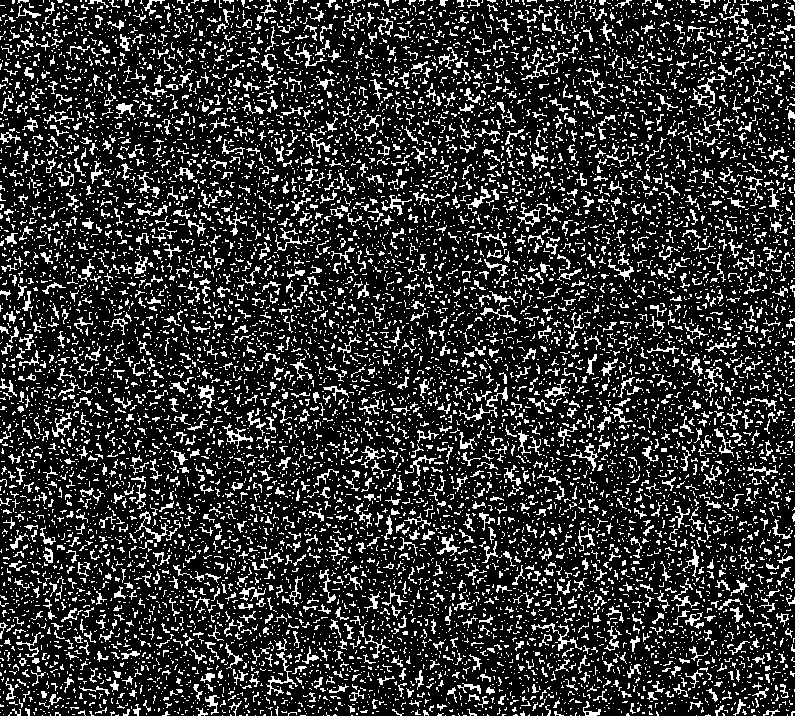
\includegraphics[width=5.8cm]{Immagini/WhiteNoiseArt.pdf}\\ \bigskip\bigskip\bigskip\bigskip\bigskip\bigskip
{\textbf{A.A. 2016/2017}}}

\begin{document}
\maketitle
\null
\thispagestyle{empty}
\clearpage
\setcounter{page}{1}
\setcounter{secnumdepth}{-2}

% Index
\tableofcontents{}
\newpage

%Exercises

\null \newpage

\section{Introduzione e nota sui linguaggi di programmazione utilizzati}

La seguenta raccolta di esercizi svolti costituisce buona parte della prova d'esame per il corso di \emph{Analisi Statistica dei Dati} presso il Dipartimento di Fisica dell'Università degli Studi di Milano-Bicocca. I sette esercizi assegnati spaziano grosso modo tra tutti gli argomenti affrontati durante tale corso semestrale e rappresentano esempi applicativi delle tecniche illustrate a lezione. Gli ambiti in cui tali applicazioni si inseriscono sono piuttosto variegati, da esercizi molto formali e astratti, quali la ricerca di minimi globali di celebri funzioni "patologiche" o il calcolo di integrali per mezzo di tecniche Montecarlo, a vere e proprie analisi dati su esperimenti (simulati) di ottica e fisica delle particelle. Non manca naturalmente una buona palestra su tutti quei fondamenti di matematica numerica e scienza dei calcolatori che costituiscono il necessario precedente (tecno)logico per qualsiasi moderna pratica di analisi statistica dei dati.\\

\noindent La natura intrinsecamente multidisciplinare della materia trattata nonché la marcata disomogeneità che caratterizza i differenti percorsi di una laurea magistrale in fisica fanno sì che la modalità di svolgimento degli esercizi sia sostanzialmente molto libera nella scelta degli approcci e degli strumenti di cui avvalersi. Personalmente ho dunque scelto di utilizzare per lo svolgimento di tutti gli esercizi dei linguaggi di programmazione \emph{interpretati} e con una sintassi di \emph{alto livello} . Tale scelta è chiaramente mirata alla flessibilità e all'immediatezza di scrittura che a mio parere un'attività di lavoro così eterogenea intrinsecamente richiede.  In particolare ho implementato quasi tutto in \texttt{Phyton}, linguaggio piuttosto moderno ma ormai caro agli ambienti della ricerca scientifica, con il vezzo di qualche incursione nel mondo di \texttt{R}, habitat ideale per qualunque applicazione di statistica e \emph{data science}. Maggiori informazioni possono essere facilmente reperite nei rispettivi siti ufficiali: \url{www.python.org} e \url{www.r-project.org}, fermo restando che la documentazione specifica di eventuali funzioni e pacchetti particolari sarà citata nel corpo della presentazione, sotto forma di nota a piè di pagina (con link). Disseminati lungo il testo saranno anche i listati di tutti gli \emph{script} implementati, con specificato il linguaggio e evidenziata opportunamente la relativa sintassi. L'indice dei codici listati può essere consultato a pagina~\pageref{listoflistings}.\\

\bigskip

\noindent Trieste, \today\\

\newpage
\section{Esercizio 1}

\begin{enumerate}[label=\Alph*.]
	
	\item Si costruisca un generatore di numeri casuali distribuiti secondo una densità di Breit-Wigner.
	\item Costruito un generatore di  numeri casuali uniforme tra 0 e 10 si discuta dei possibili test di casualità utilizzabili per le sequenze prodotte.
		
\end{enumerate}

\[* * * \] \smallskip

\noindent Per generare numeri distribuiti secondo la densità di probabilità di Breit-Wigner possiamo utilizzare il \emph{metodo della cumulante}: detta $f(x)$ la distribuzione di interesse e detta $F(x) $ la sua funzione cumulante\footnote{Ossia $F(x)$ sia definita come: $$ F(x) = \int_{-\infty}^{x} f(x')\mathop{dx'} $$}, il problema viene ricondotto alla generazione di numeri casuali \emph{uniformi} nell'intervallo $[0,1]$, che risultano essere in corrispondenza biunivoca con la sequenza desiderata attraverso la funzione inversa della cumulante.\\

\noindent Ciò è garantito dal seguente risultato generale: la variabile casuale $\xi = F(x)$ è distribuita secondo una densità di probabilità $g(\xi)$ data da


\begin{align*}
g(\xi) &= f(x) \cdot \left|\frac{dx}{d\xi}\right| \\ 
&=  f(x) \cdot \left|\frac{d\xi}{dx}\right|^{-1} \\ 
&=  f(x) \cdot \left|\frac{d}{dx}\int_{-\infty}^{x} f(x')\mathop{dx'}\right|^{-1} \\ \\
&= f(x) \cdot \left|f(x)\right|^{-1}  \\ \\
&= 1. 
\end{align*}

\noindent Dal momento che, per definizione di cumulante, si ha $ \xi  \in [0,1]$ risulta evidente che $\xi$ ha distribuzione uniforme nell'intervallo $[0,1]$, per cui possiamo ottenere delle $x$ distribuite secondo la densità $f(x)$ dalla relazione:

$$x = F^{-1}(\xi),$$
	
\noindent con $\xi$ numeri casuali opportunamente generati per avere distribuzione uniforme in $[0,1]$.\\

\noindent Nel nostro caso la procedura è piuttosto semplice dal momento che la distribuzione di Breit-Wigner ha cumulante calcolabile analiticamente:

\begin{align*}
f_{_{\mathrm{BW}}}(x) &= \frac{\Gamma}{\pi(\Gamma^2 + (x-x_0)^2)} \\ \\
F_{_{\mathrm{BW}}}(x) &= \frac{1}{\pi}\arctan\left[\frac{x-x_0}{\Gamma}\right] + \frac{1}{2}
\end{align*}

\noindent con $x_0$ valore corrispondente al picco centrale della distribuzione e $\Gamma$ sua larghezza HWHM (Cfr. Figura~\ref{fig:Breit-Wigner}).\\

\begin{figure}
	\centering
	\caption{Distribuzione di Breit-Wigner per $\Gamma=1$ e $x_0=0$.}
	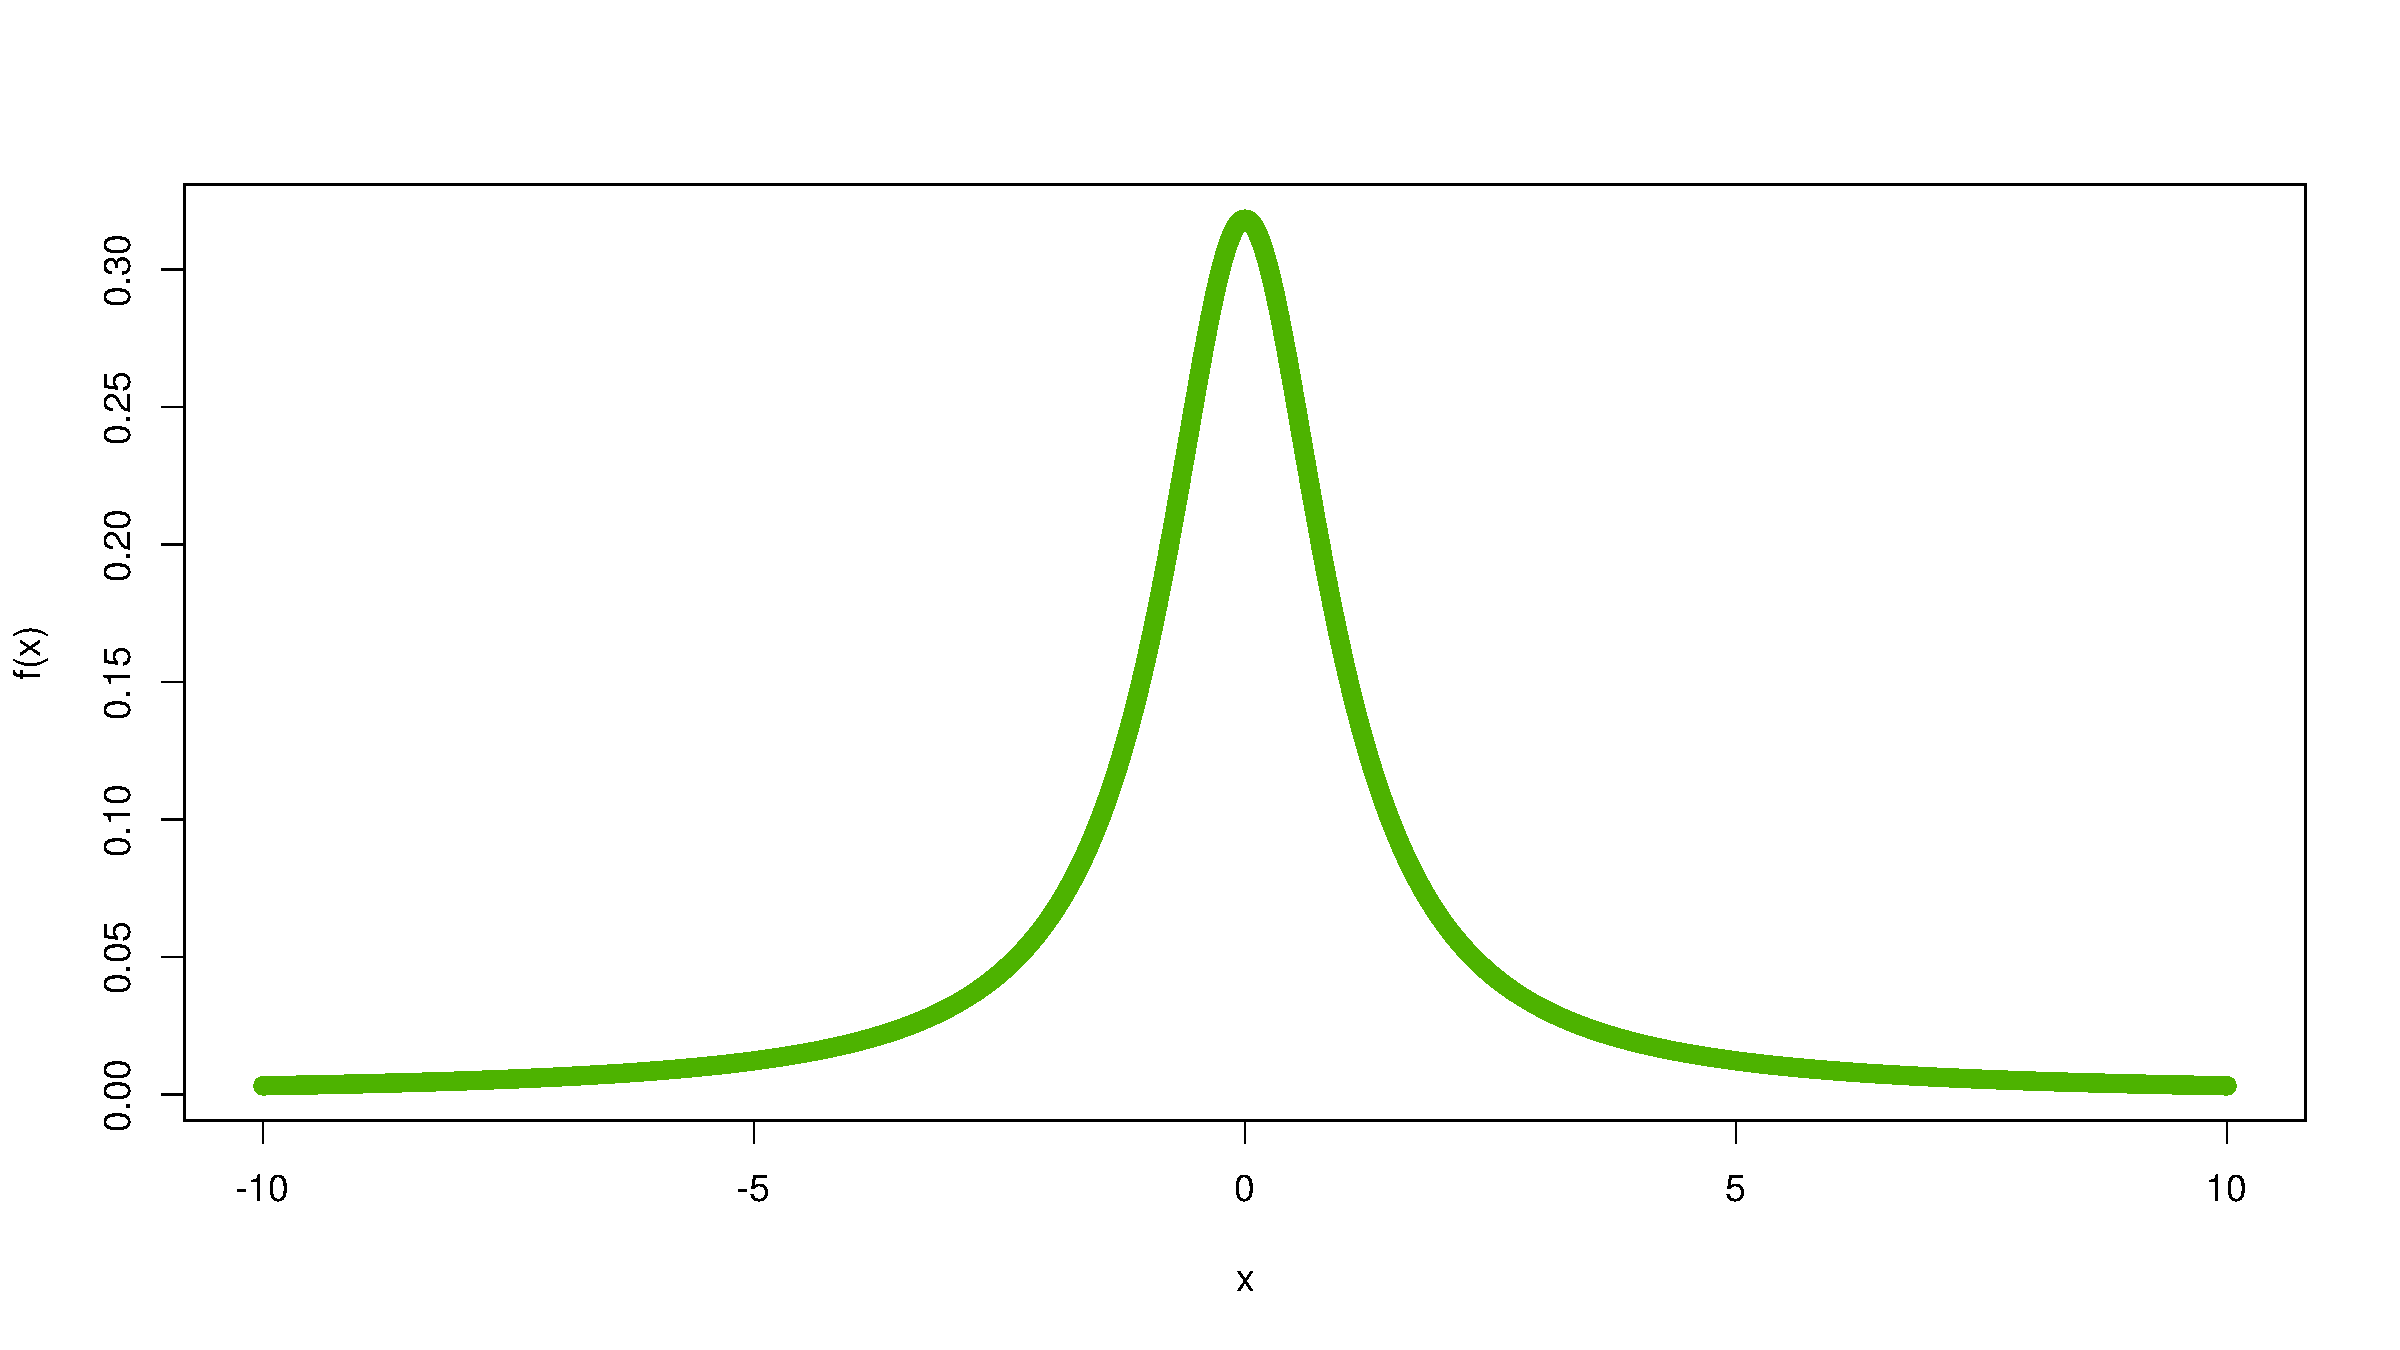
\includegraphics[width=.98\textwidth, trim={0 1cm 0 2.5cm},clip]{Immagini/Breit-Wigner.pdf}
	\label{fig:Breit-Wigner}
\end{figure}

\noindent Pertanto invertendo la relazione

$$ \xi = \frac{1}{\pi}\arctan\left[\frac{x-x_0}{\Gamma}\right] + \frac{1}{2}$$

\noindent otteniamo l'equazione desiderata:

$$\boxed{x = x_0 + \Gamma\tan\left[\pi\left(\xi-\frac{1}{2}\right)\right]}$$\\

\noindent Per generare i numeri casuali $\xi$ si è utilizzato il pacchetto \texttt{RNG} dell'ambiente statistico \texttt{R}, che permette di ottenere sequenze pseudo-random con periodo pari a $(2^{19937} - 1)$, per mezzo di un generatore di tipo "Twisted GFSR".\footnote{In particolare il pacchetto permette di eseguire svariati algoritmi per la generazione delle sequenze pseudo-random, selezionati specificando il parametro \texttt{rng.kind} nel codice.  L'opzione di default implementa l'algoritmo \emph{Marsenne-Twister}, sviluppato nel 1998 da Matsumoto e Nishimura [ACM article: \href{https://doi.org/10.1145/272991.272995}{\texttt{doi:10.1145/272991.272995}}].\\
Per maggiori dettagli sul pacchetto \texttt{RNG}: \url{https://stat.ethz.ch/R-manual/R-devel/library/base/html/Random.html}}\\

\noindent In Figura~\ref{fig:Es1A_Results} è rappresentato l'istogramma relativo a $N=10^5$ estrazioni di $x$, raggruppate in $50$ bins, con parametri Breit-Wigner $x_0 = 0$ e $\Gamma = 1$. L'ottima sovrapposizione con il grafico analitico della $f_{_{\mathrm{BW}}}(x)$ conferma la bontà del metodo implementato.\footnote{Per quanto riguarda i limiti di affidabilità dell'algoritmo proposto si tenga presente che il numero di estrazioni $N$ non dovrà mai essere comparabile con il periodo di ripetizione del generatore pseudo-random adoperato.}\\

\begin{figure}
	\centering
	\caption{Uno degli istogrammi generati a confronto con il grafico analitico della distribuzione.}
	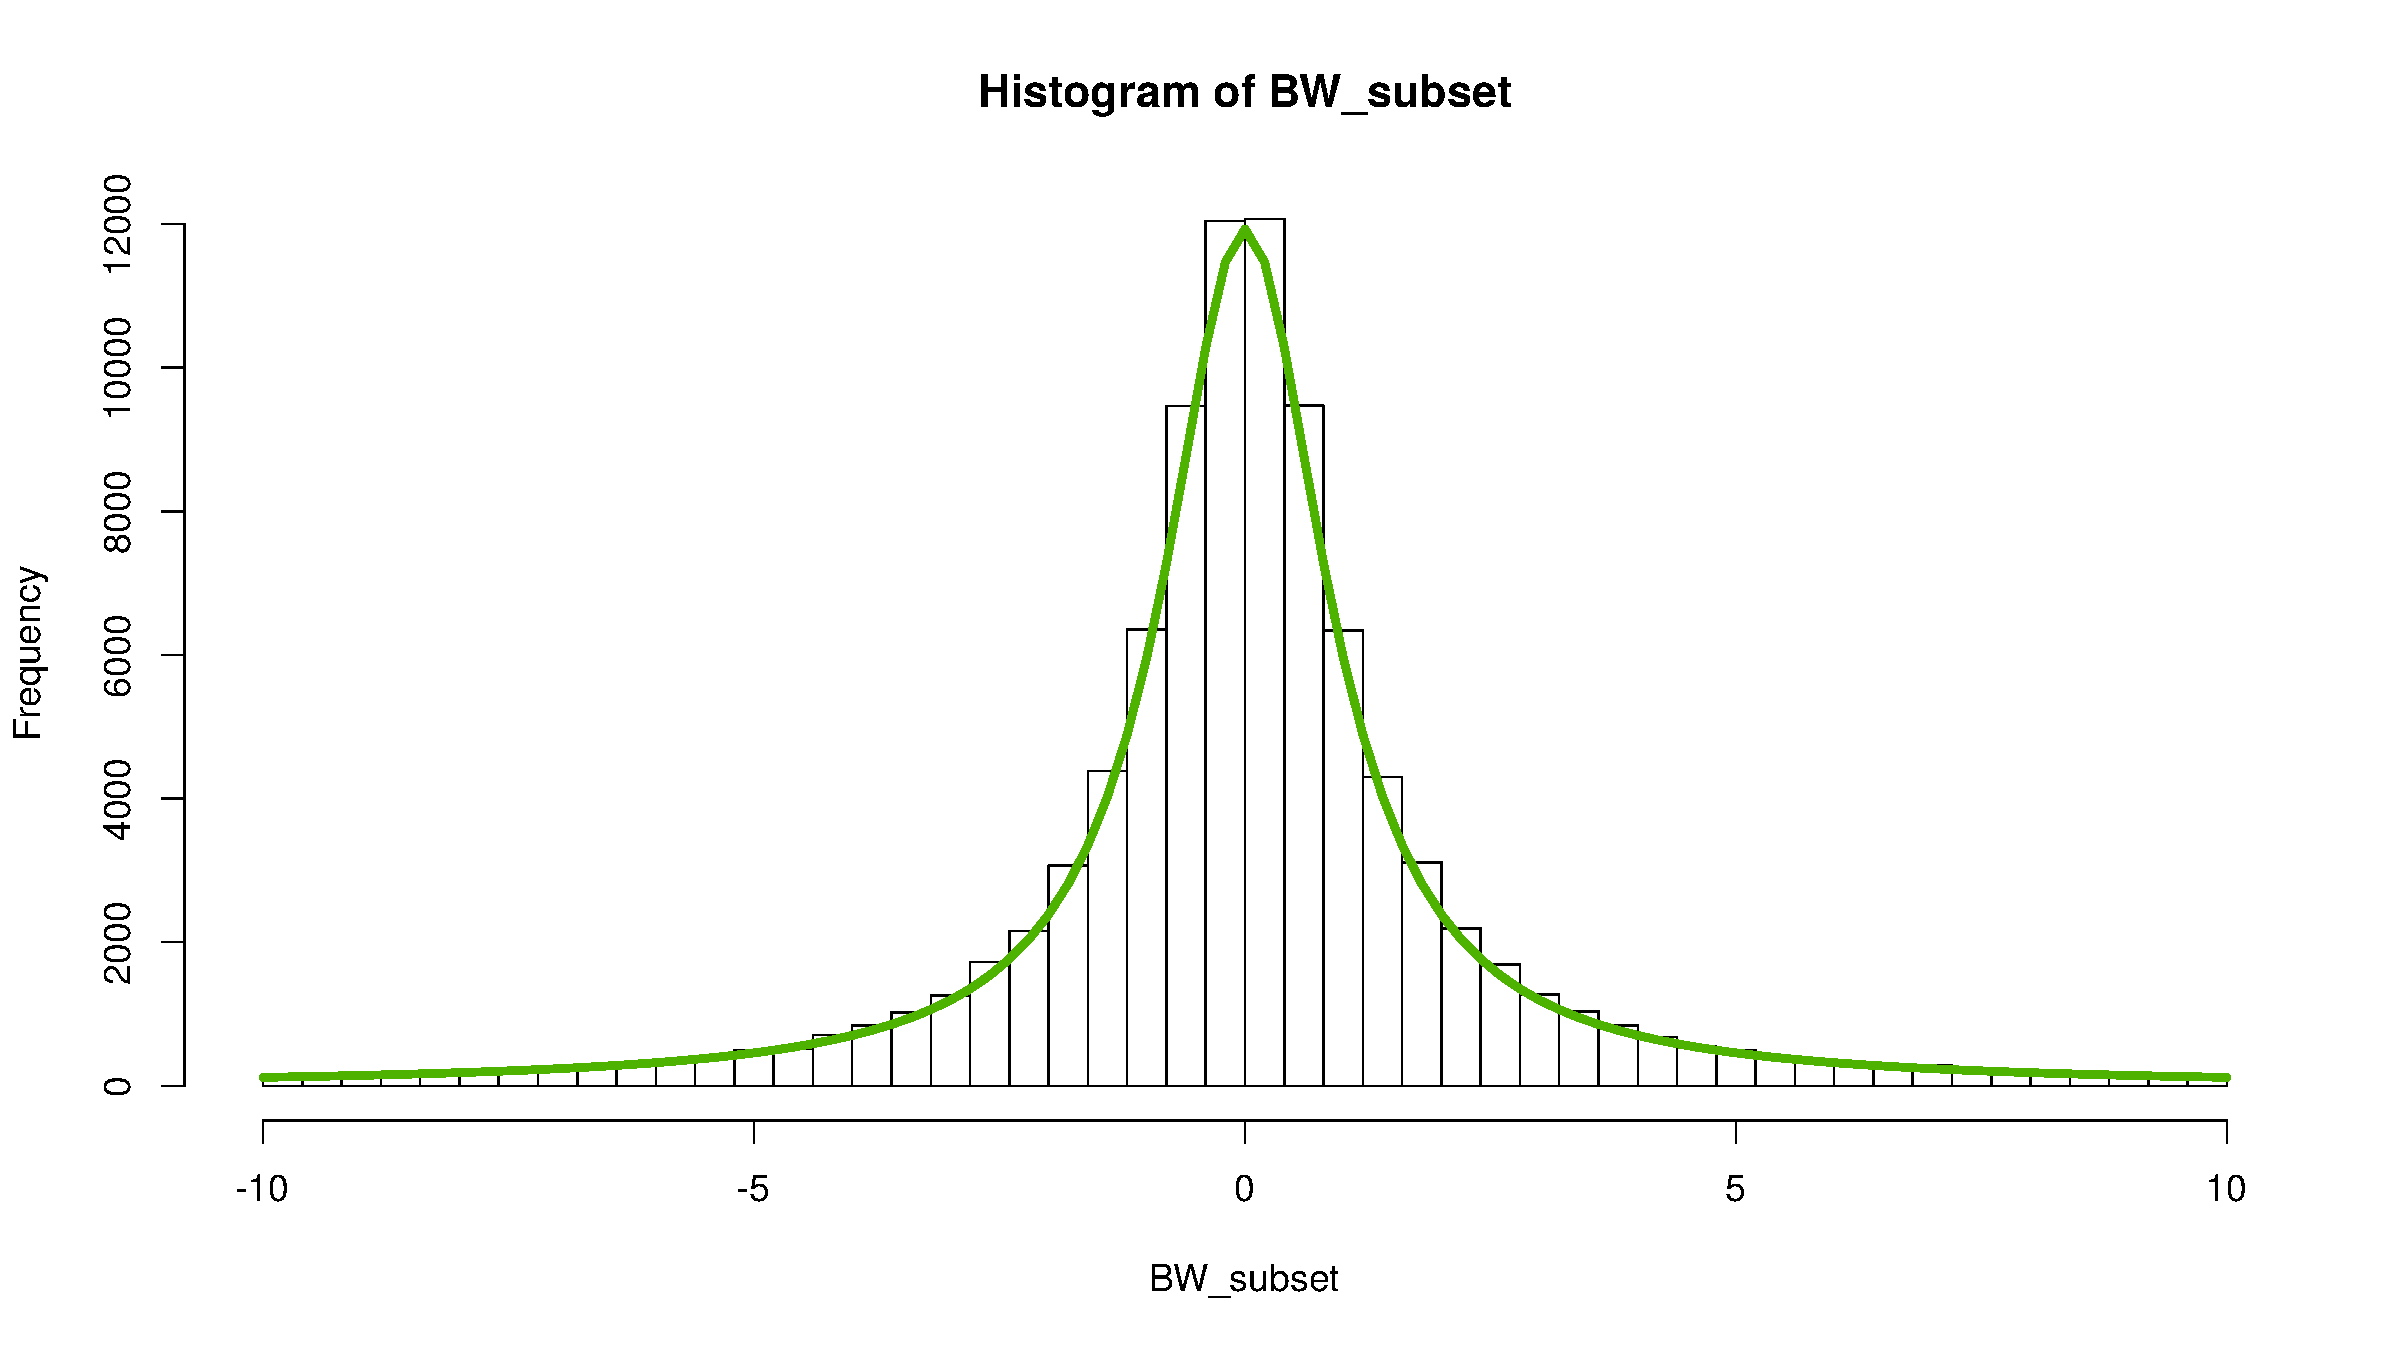
\includegraphics[width=\textwidth, trim={0 1cm 0 2.3cm},clip]{Immagini/BW_histogram.pdf}
	\label{fig:Es1A_Results}
\end{figure}

\noindent Di seguito viene riportato il listato del codice \texttt{R} utilizzato:

\begin{lstlisting}[language=R, style=Rstyle, caption=\texttt{R} code for Exercise 1/A (to generate a Breit-Wigner histogram), xleftmargin=.02\textwidth]
# Entering here the desired Breit-Wigner parameters:
x0 = 0
HWHM = 1

# Setting here an appropriate x domain (as a linear spaced vector)
x = seq(-10, 10, by = 0.04) # Note that "by" fixes the number of bins

# Defining the Breit-Wigner function
f_x = HWHM / (pi*HWHM^2 + pi*(x-x0)^2)

# Plotting and saving a graph of the function
cairo_pdf('Breit-Wigner.pdf', width = 16, height = 9, pointsize = 18)
mycolor = rgb(0.3, 0.7, 0)
plot(x, f_x, xlab='x', ylab='f(x)', col=mycolor)
dev.off()

# Extracting the required N uniform random numbers (N is a parameter of choice)
N = 10^5
uniform_set = runif(N, 0, 1) 

# Using inverse-cumulant equation to get Breit-Wigner dataset
BW_set = x0 + HWHM*tan(pi*(uniform_set-1/2))
	
# Defining histogram range and bins from x vector
hist_range = range(x)
bins = x

# Retrieving a proper subset of Breit-Wigner data 
BW_subset = subset(BW_set, BW_set <= max(hist_range) & BW_set >= min(hist_range))

# Plotting and saving the histogram of Breit-Wigner dataset (with analitical check)
myhistogram = hist(BW_subset, bins)
A = (myhistogram$counts / myhistogram$density)[1] # Normalization factor
cairo_pdf('BW_histogram.pdf', width = 16, height = 9, pointsize = 18)
plot(myhistogram)
curve(A*dcauchy(x,location=x0,scale=HWHM,log=FALSE), lwd=5, add=TRUE,  col=mycolor)
dev.off()
\end{lstlisting}

\noindent Infine risulta interessante osservare come all'aumentare del numero di bin, fissato $N=10^5$, aumenti il "rumore" nell'istogramma prodotto (Cfr. Figura~\ref{fig:Breit-Wigner_BINS}). Ciò è del tutto ragionevole poiché più sono i bin e più sarà piccolo il campione su cui mediamo il valore da assegnare a ciascun bin. Possiamo quindi concludere che, fissato di converso il numero di bin che ci interessa, riprodurremo meglio la distribuzione tanti più saranno i numeri generati, come ci si aspetta. Una verifica concreta dell'equivalenza di queste due affermazioni si ha osservando la Figura~\ref{fig:Breit-WIgner_N}, che confronta due istogrammi con medesimo numero di bin ($500$) ma relativi rispettivamente a $10^5$ e $10^6$ eventi generati. Tutto ciò costituisce una verifica empirica del \textsl{Teorema del Limite Centrale}.

\captionsetup*[subfigure]{position=bottom}
\begin{figure}
	\centering
	\caption{Istogrammi generati per $N=10^5$ eventi, distribuiti in bin di numero crescente.}
	\subfloat[]{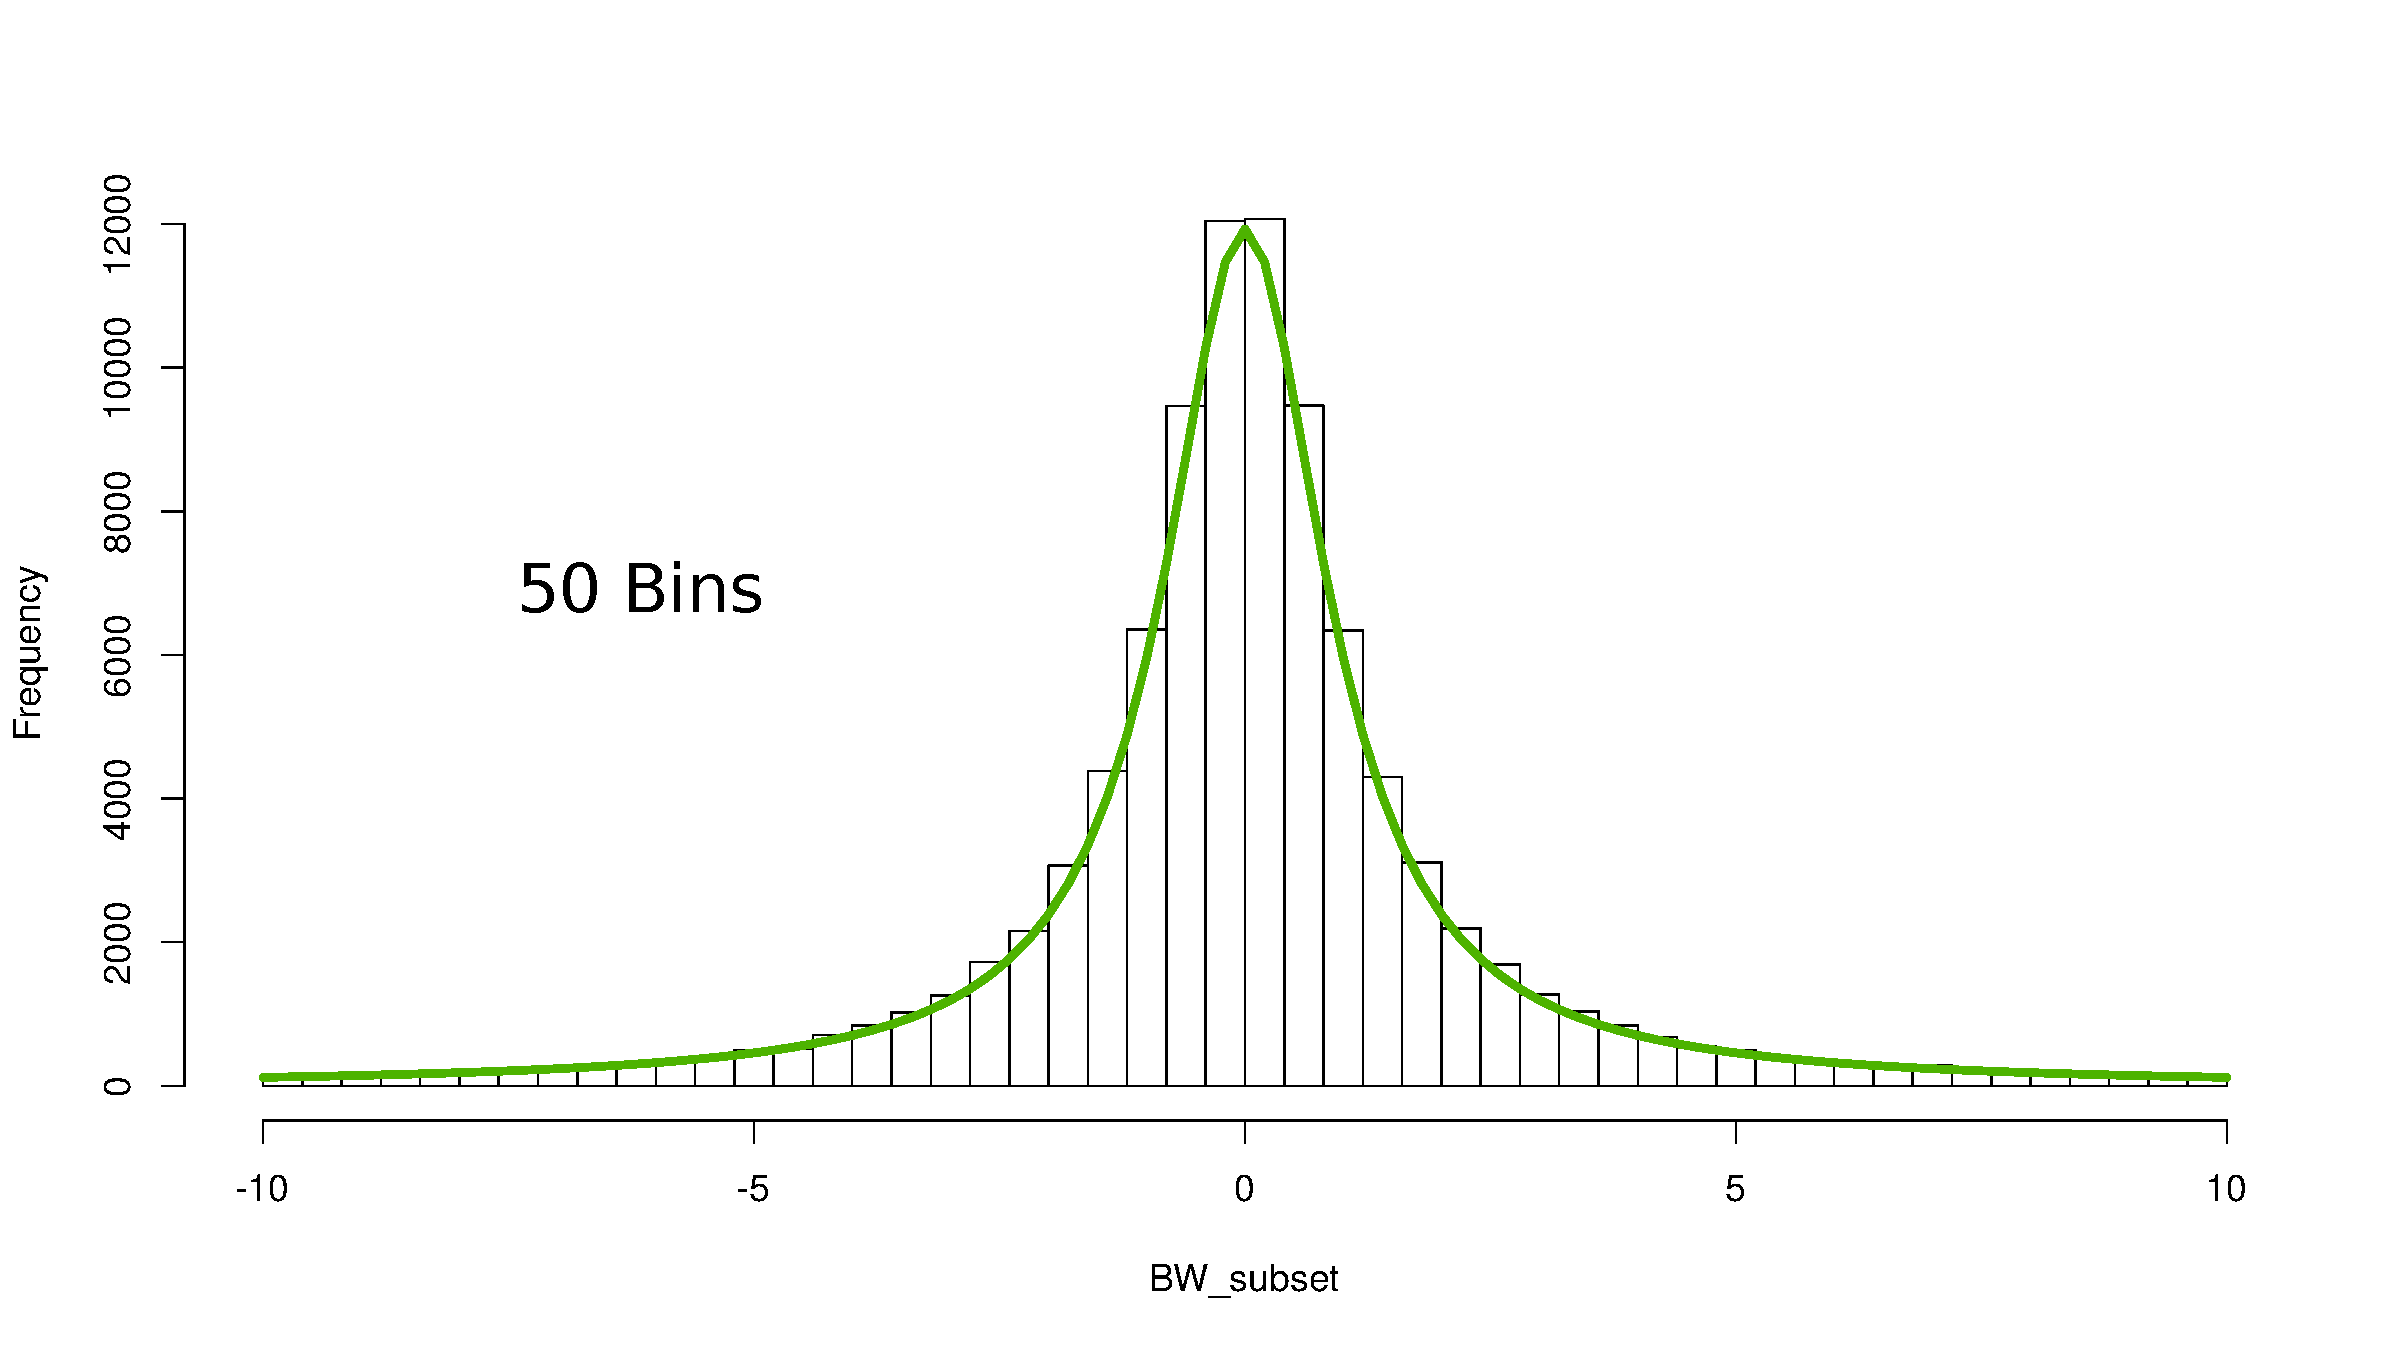
\includegraphics[width = 2.9in]{Immagini/BW_histogram_50bins.pdf}} 
	\subfloat[]{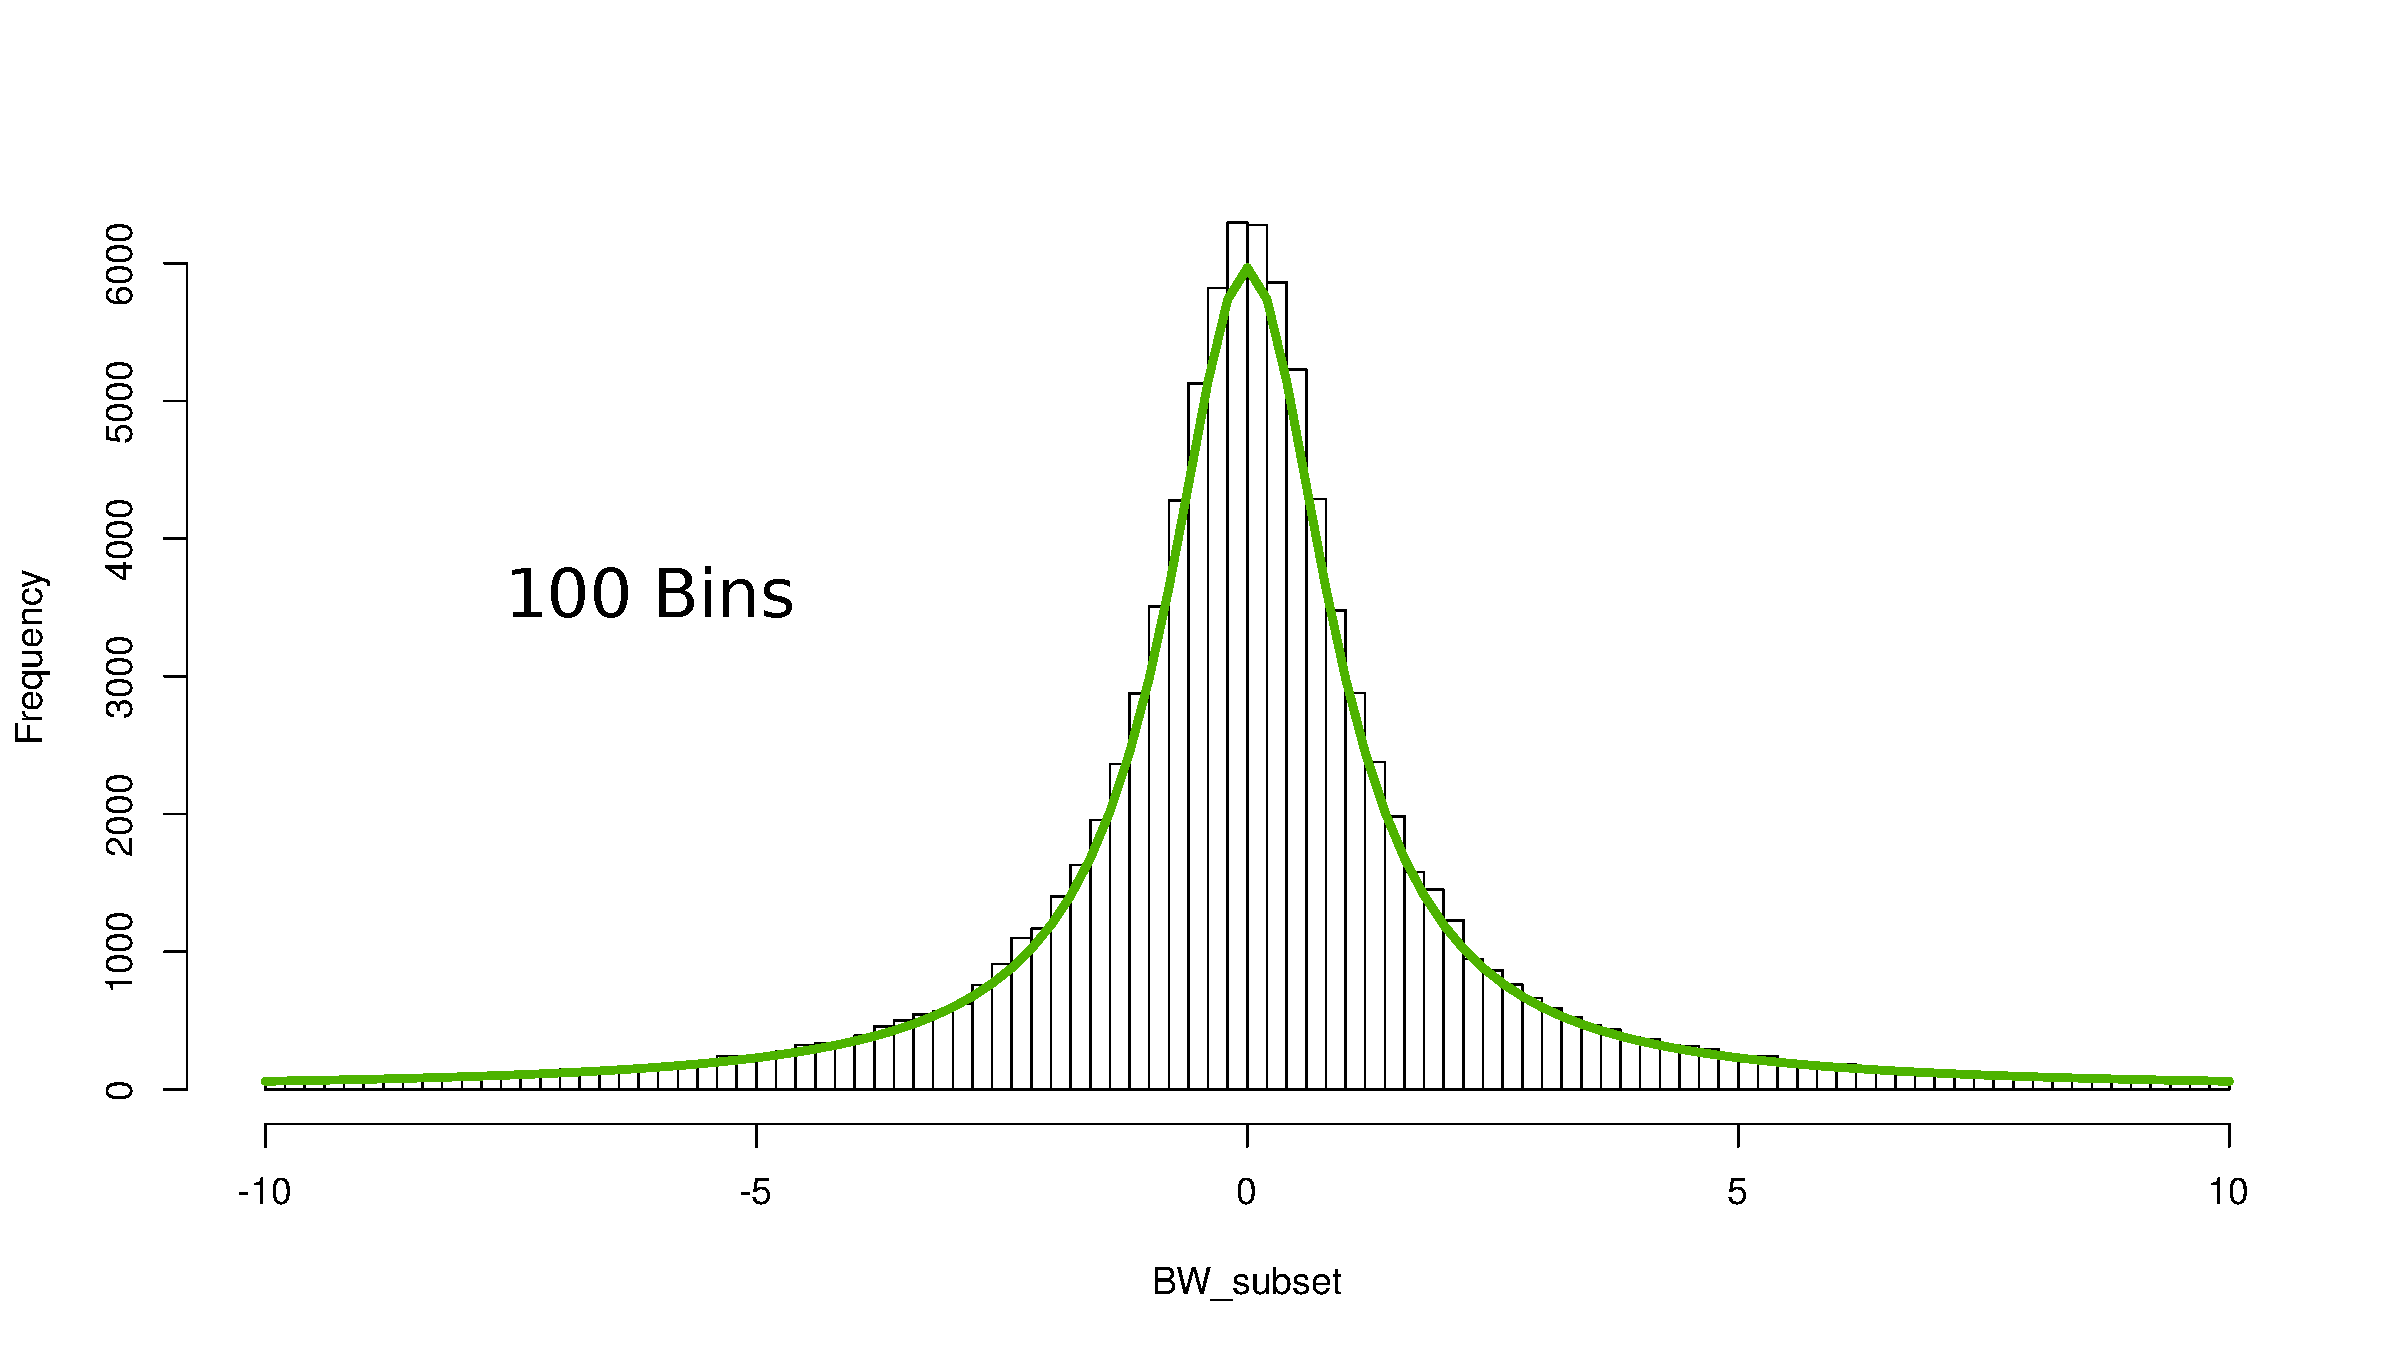
\includegraphics[width = 2.9in]{Immagini/BW_histogram_100bins.pdf}}\\
	\subfloat[]{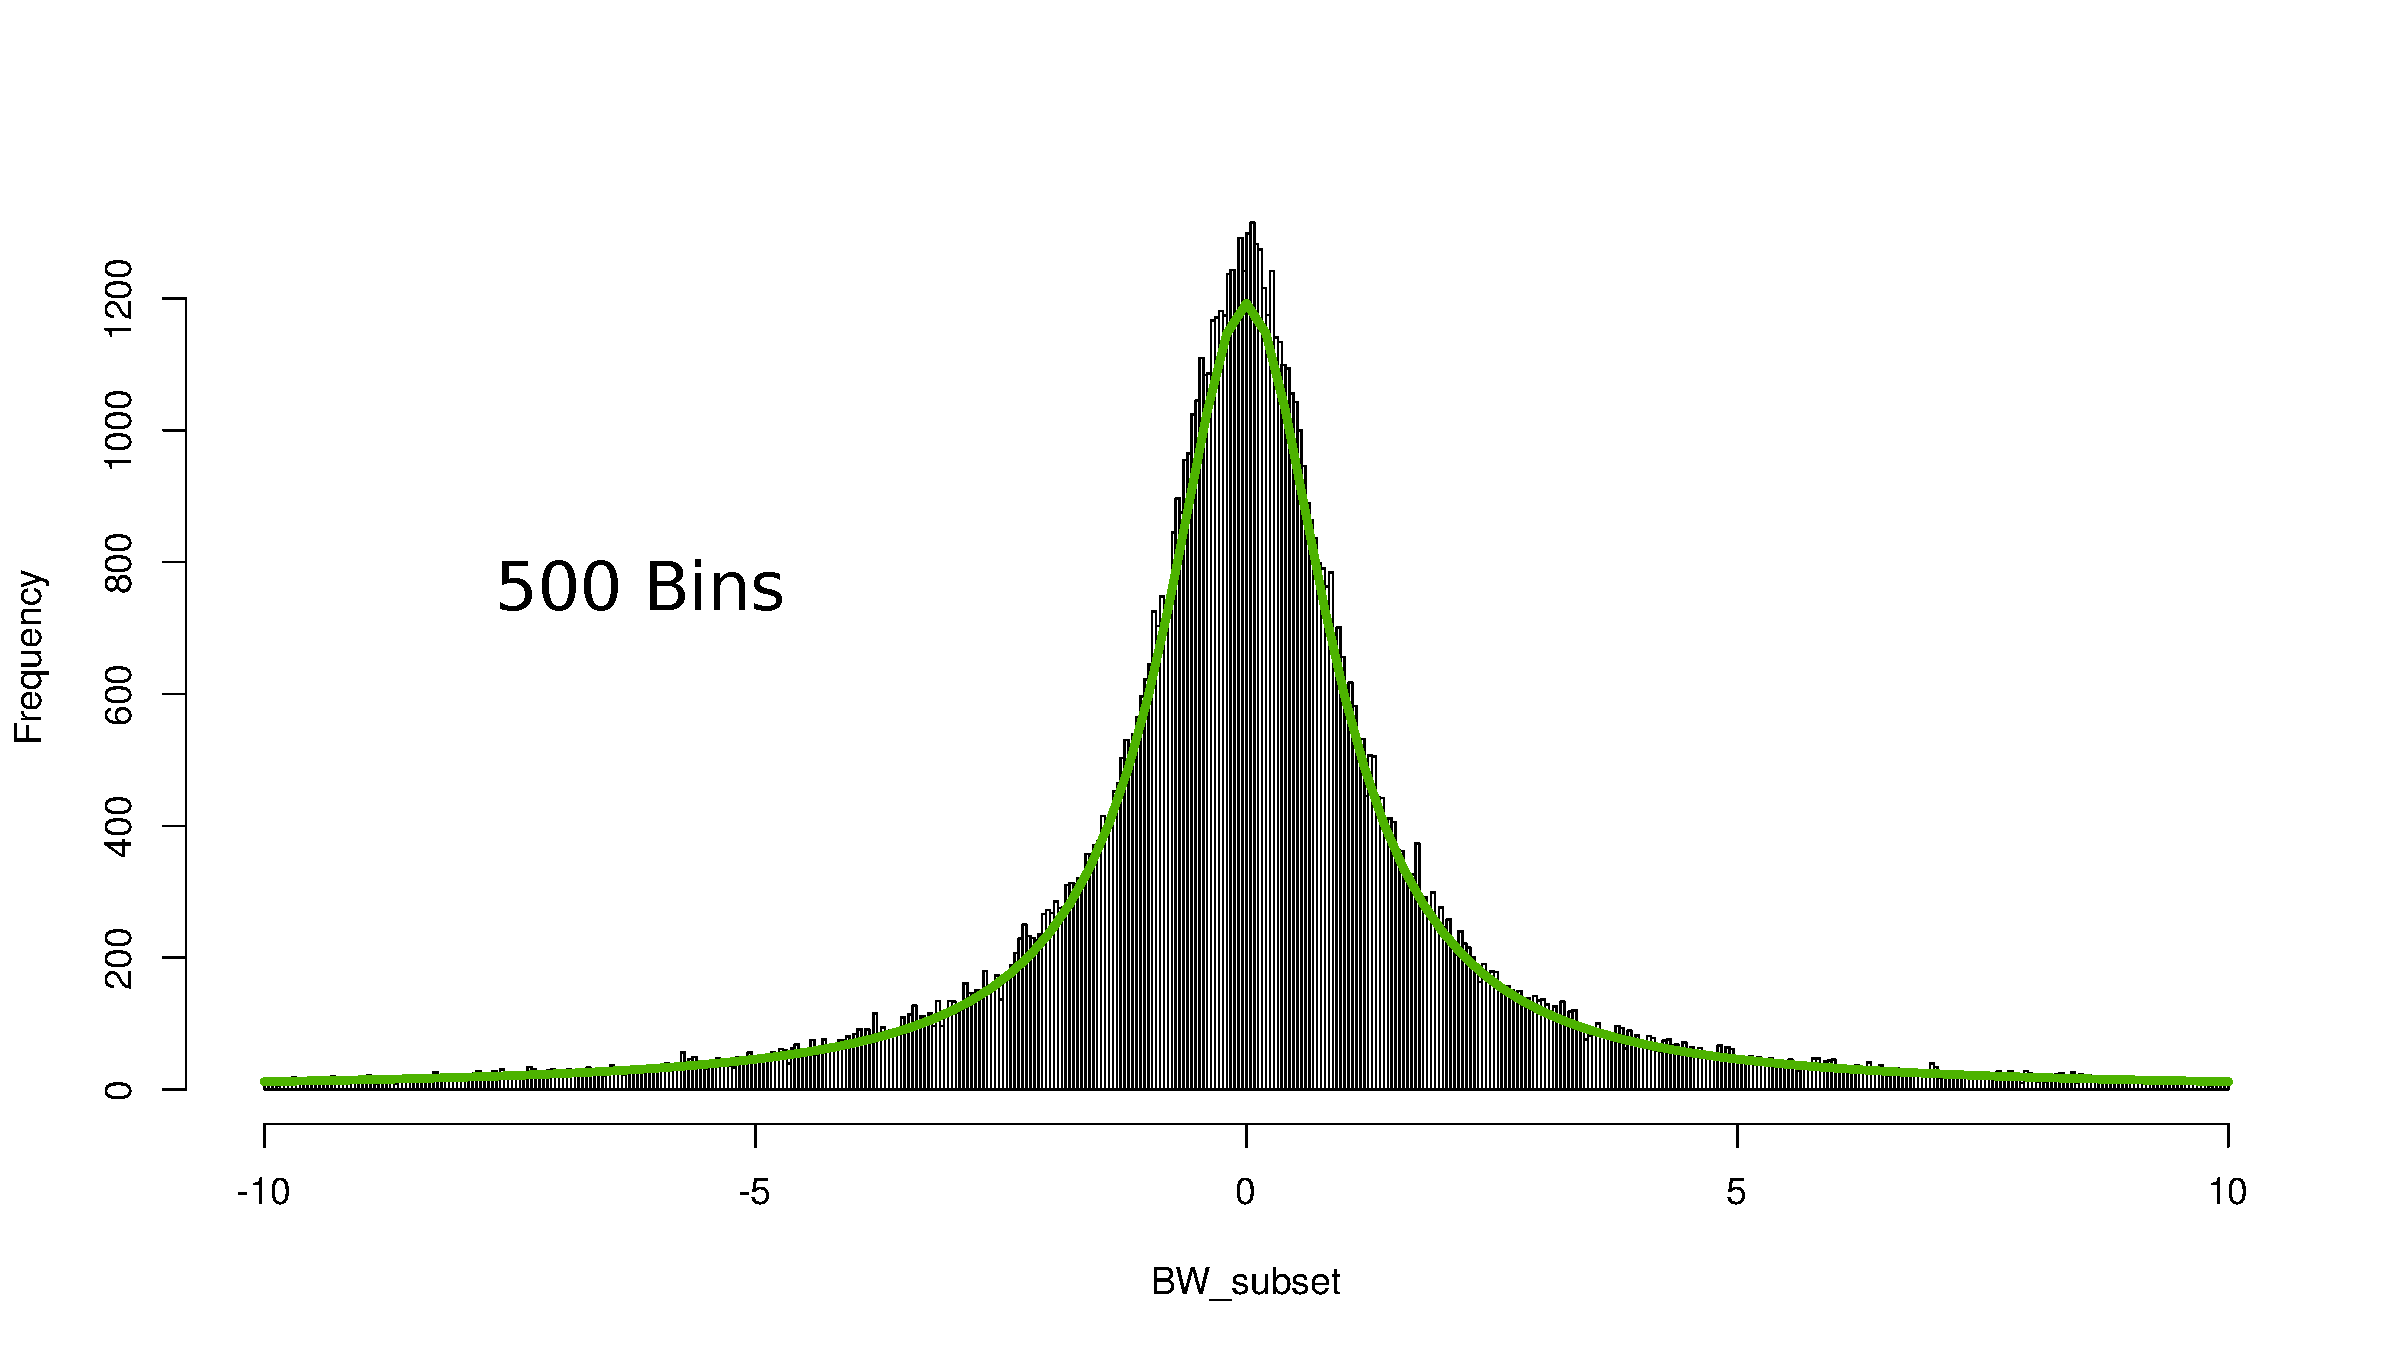
\includegraphics[width = 2.9in]{Immagini/BW_histogram_500bins.pdf}}
	\subfloat[]{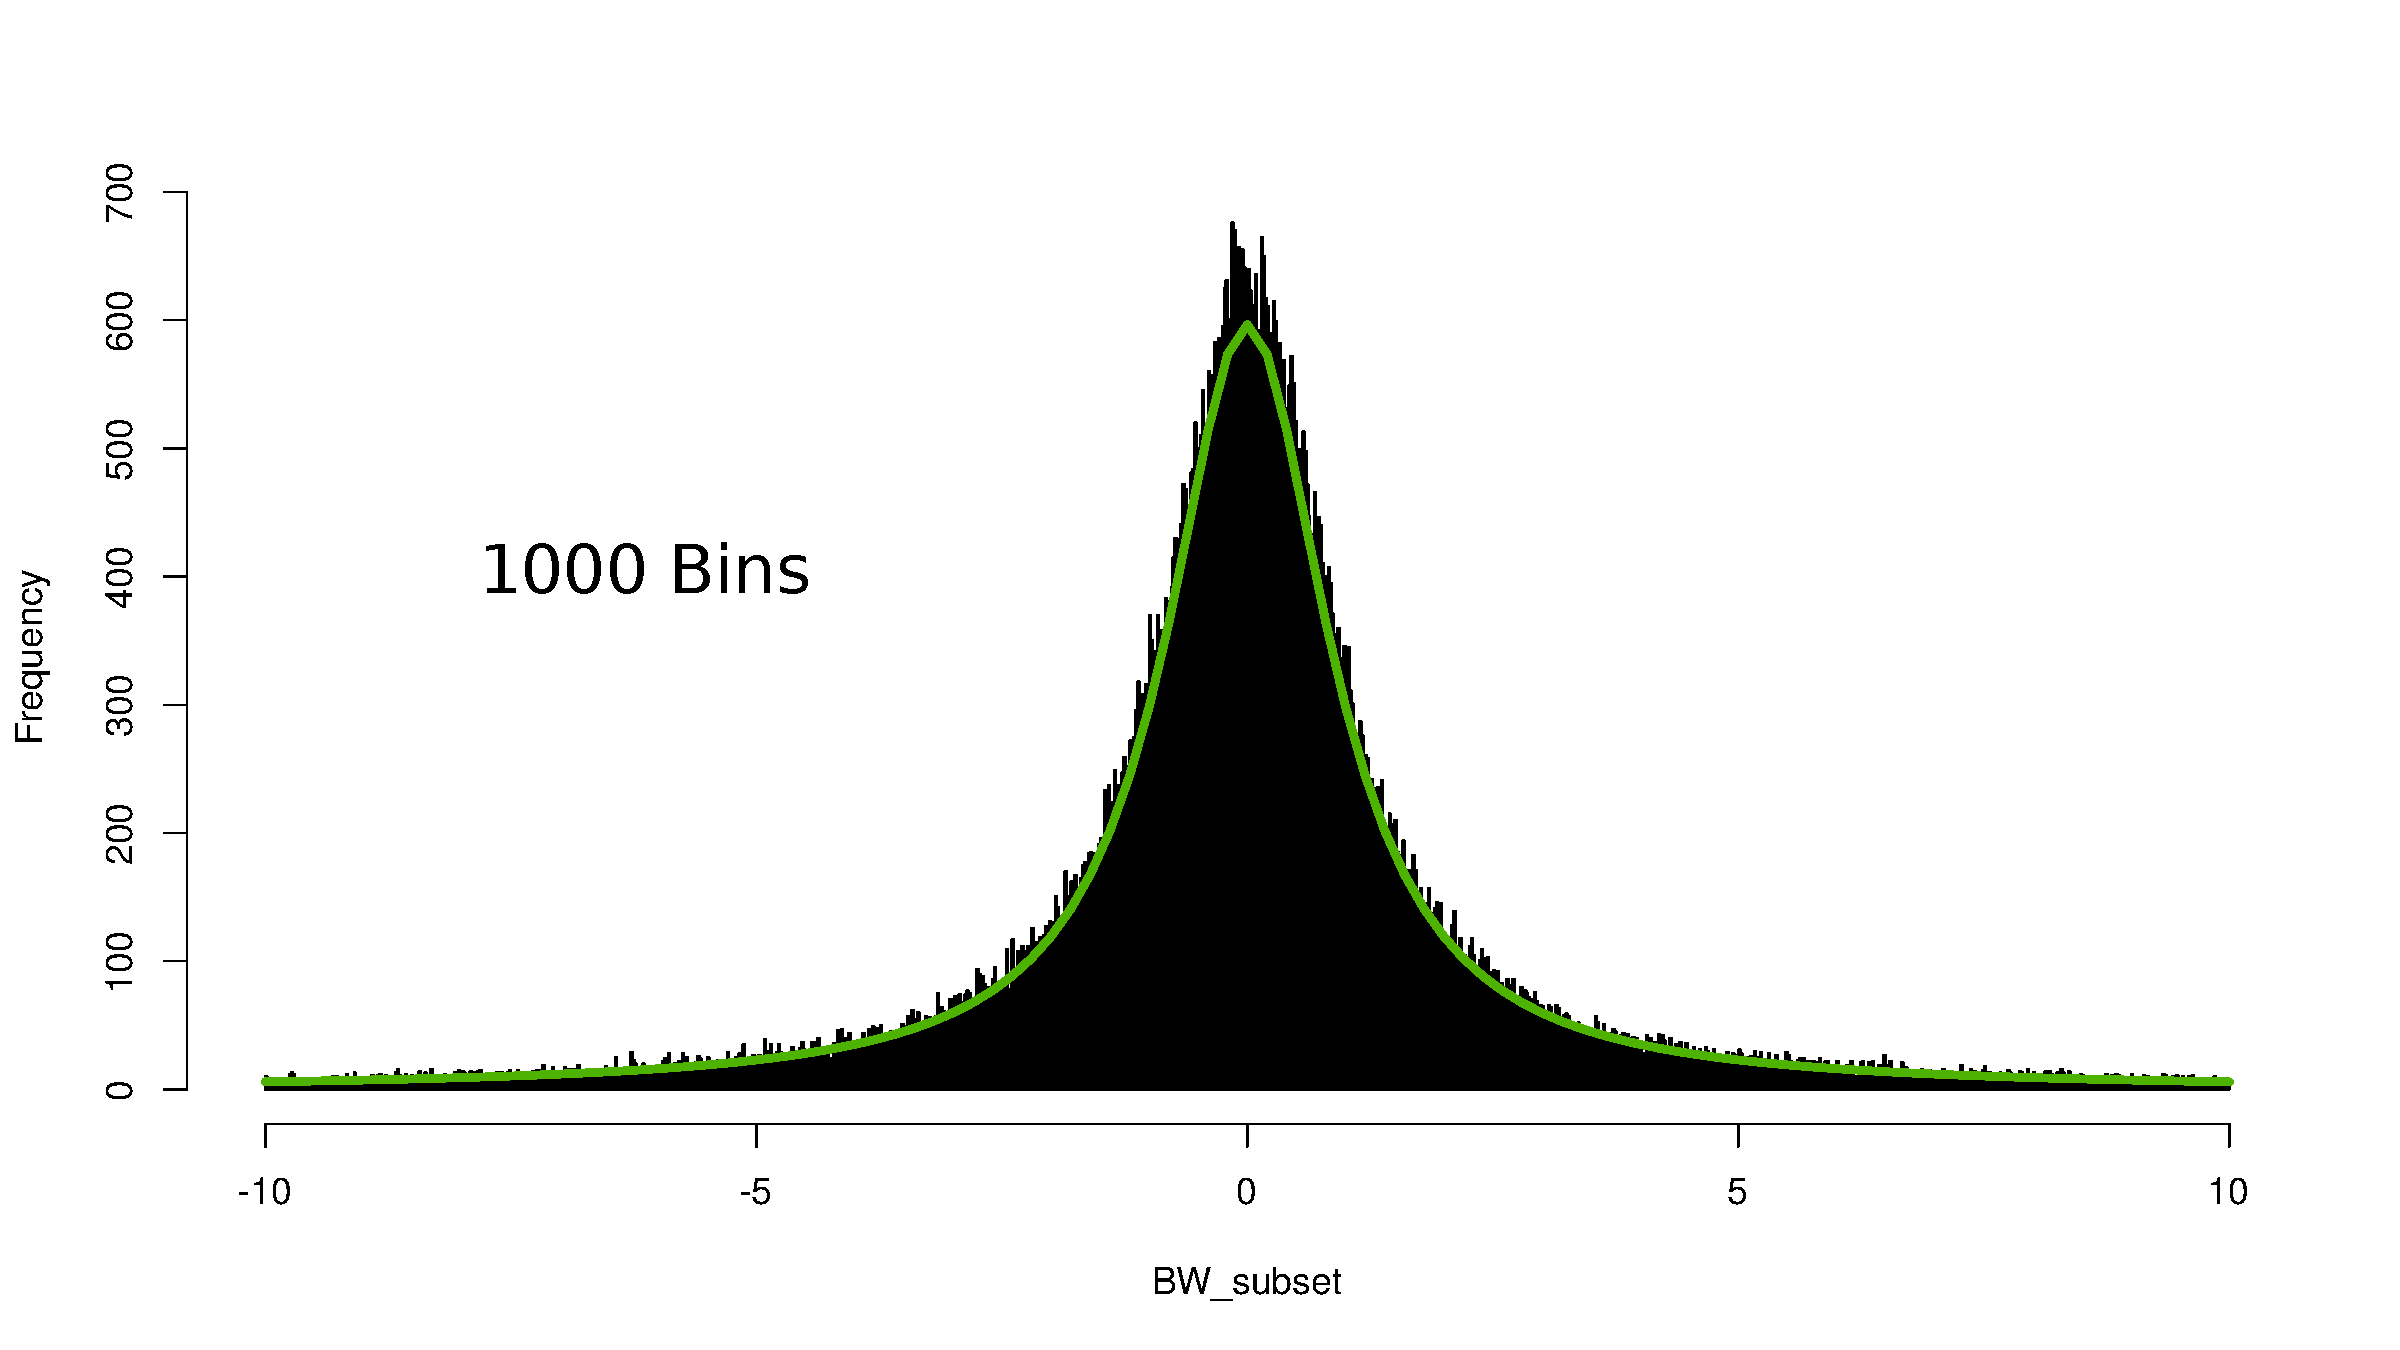
\includegraphics[width = 2.9in]{Immagini/BW_histogram_1000bins.pdf}} \\
	\subfloat[]{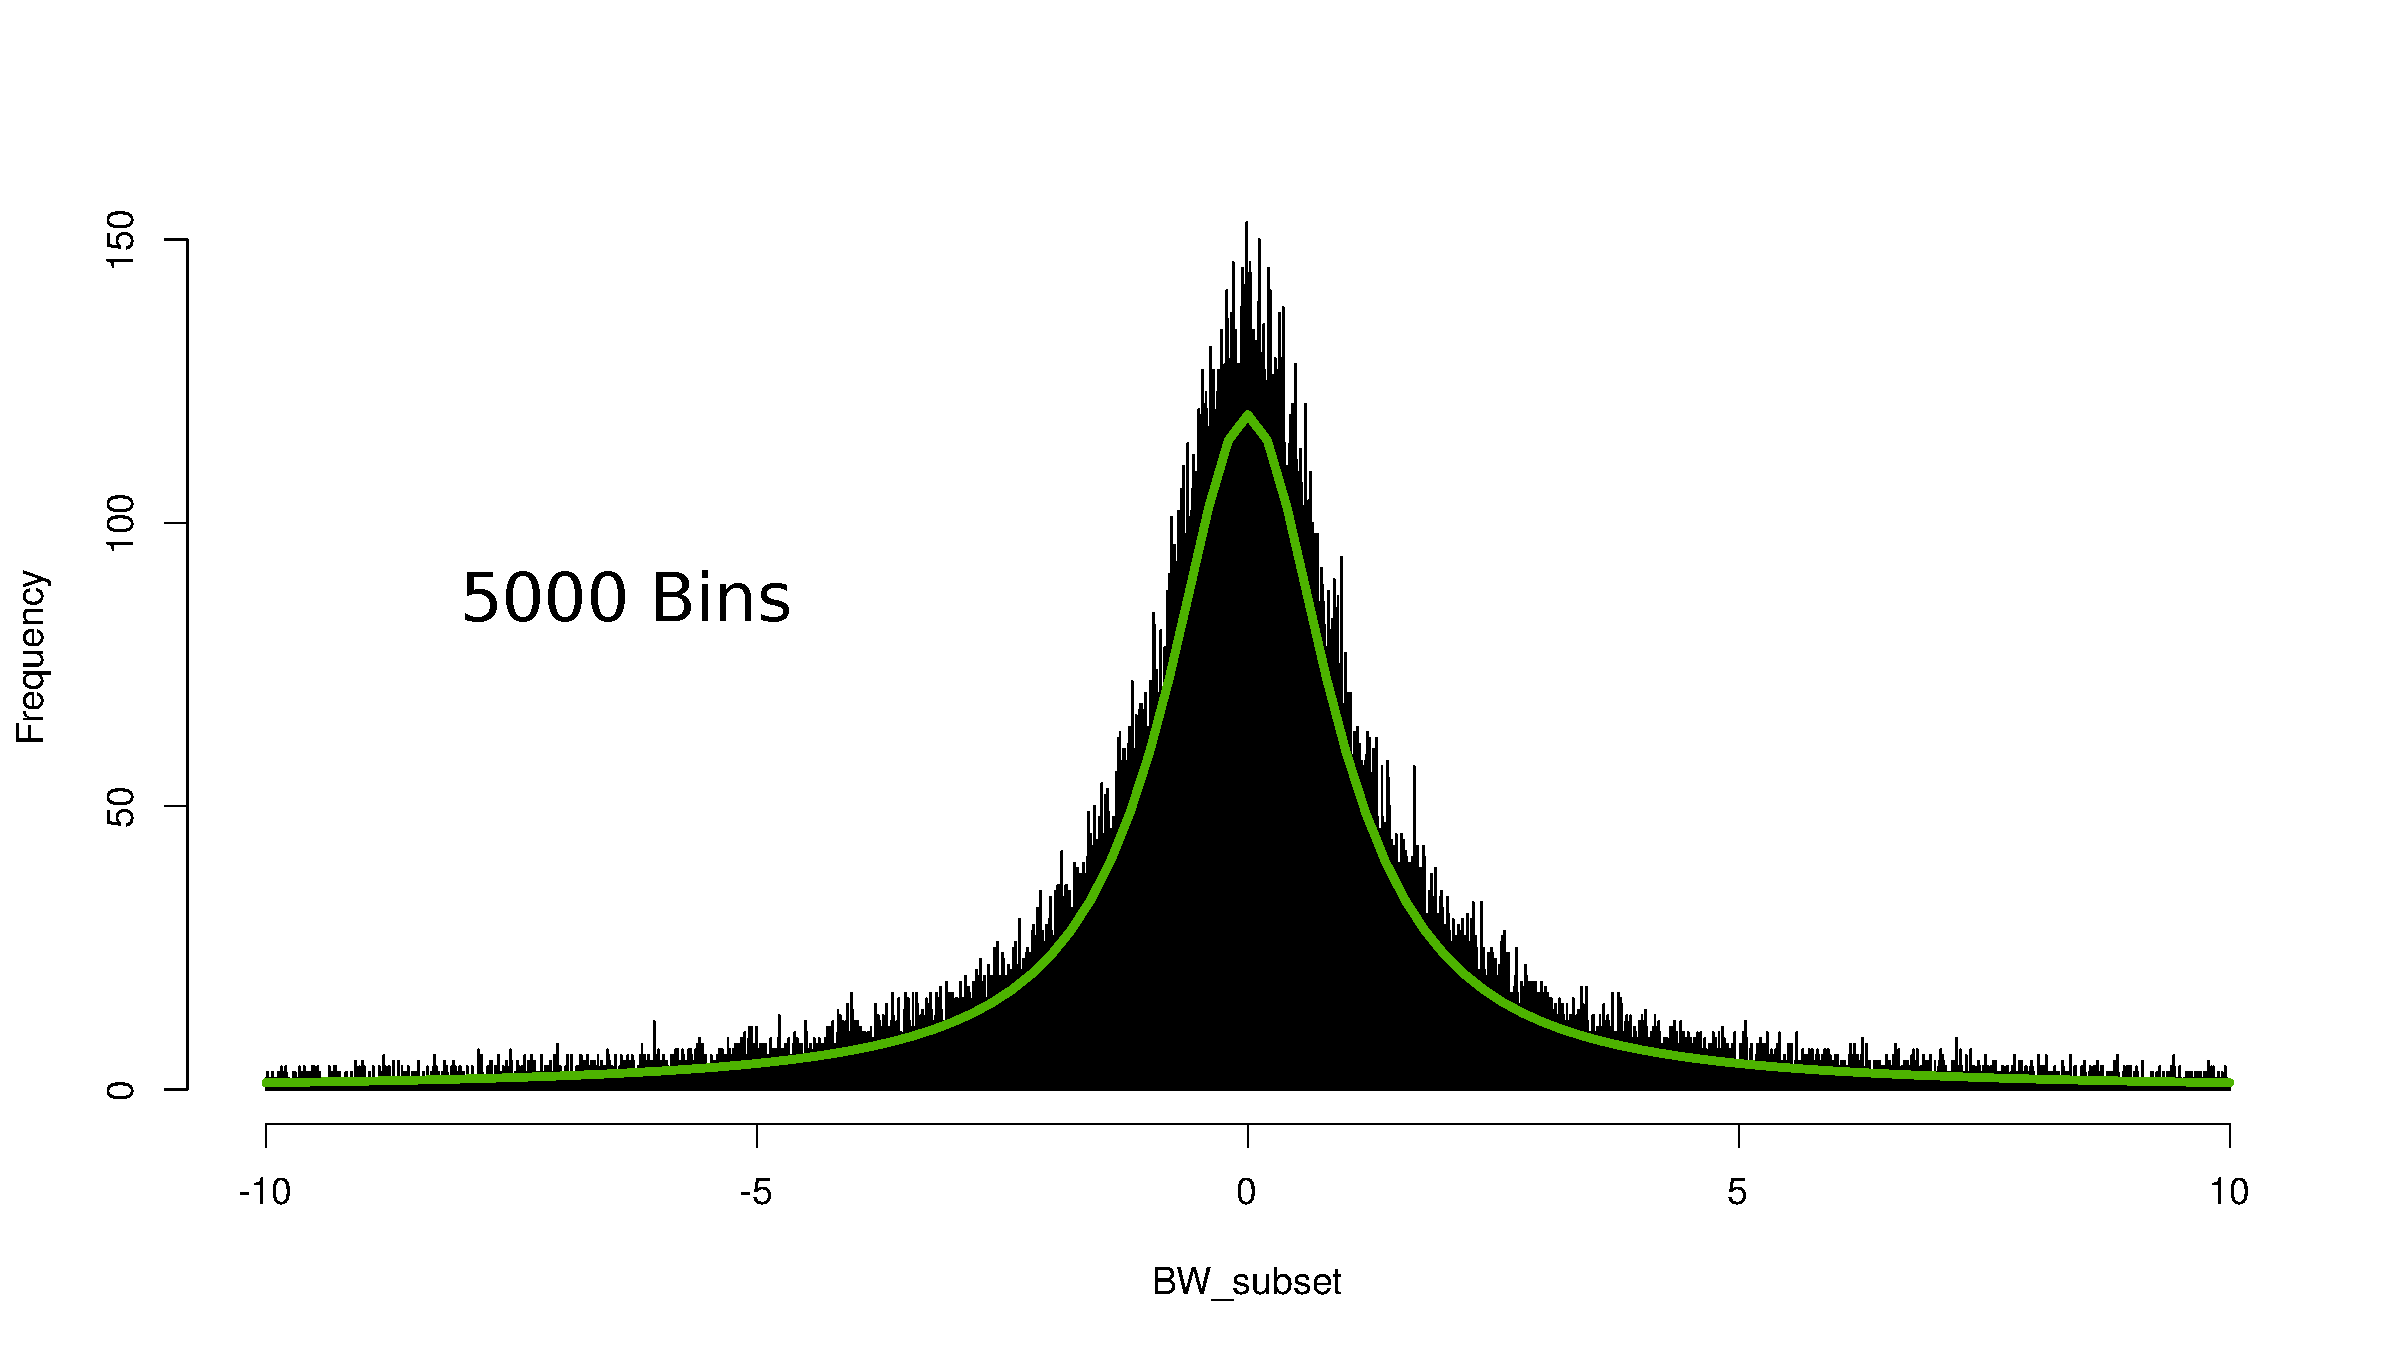
\includegraphics[width = 2.9in]{Immagini/BW_histogram_5000bins.pdf}}
	\subfloat[]{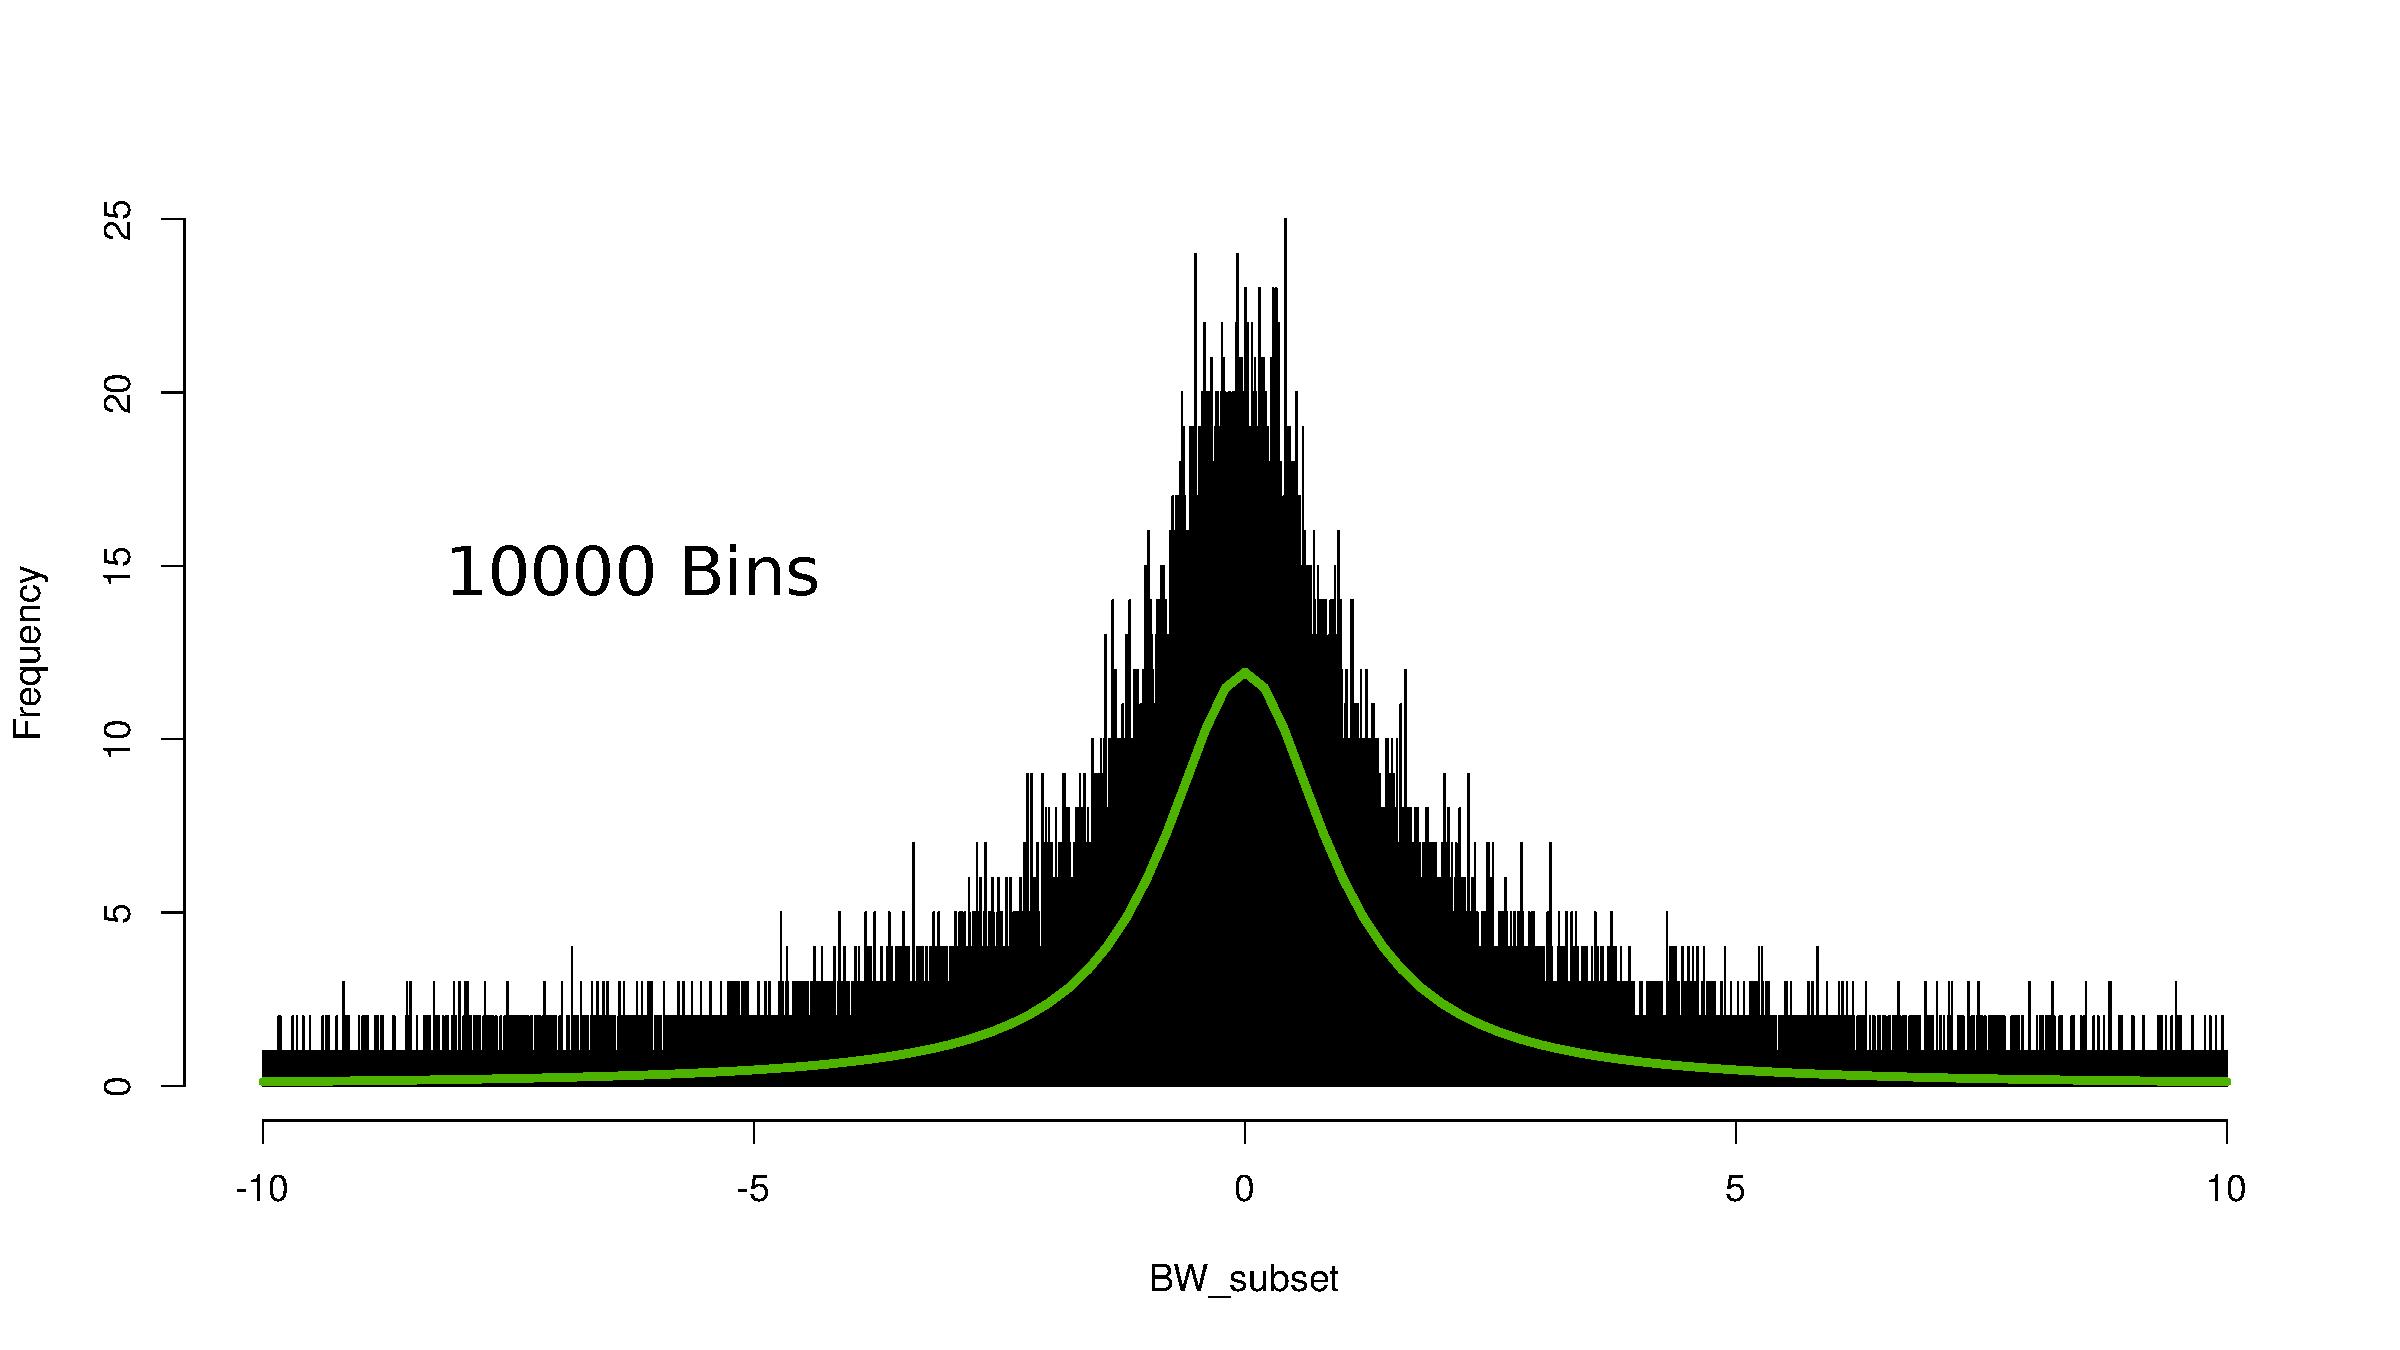
\includegraphics[width = 2.9in]{Immagini/BW_histogram_10000bins.pdf}}
	\label{fig:Breit-Wigner_BINS}
\end{figure}

\begin{figure}
	\centering
	\caption{Istogrammi generati utilizzando $500$ bin, ma con differente numero di eventi totali.}
	\subfloat[]{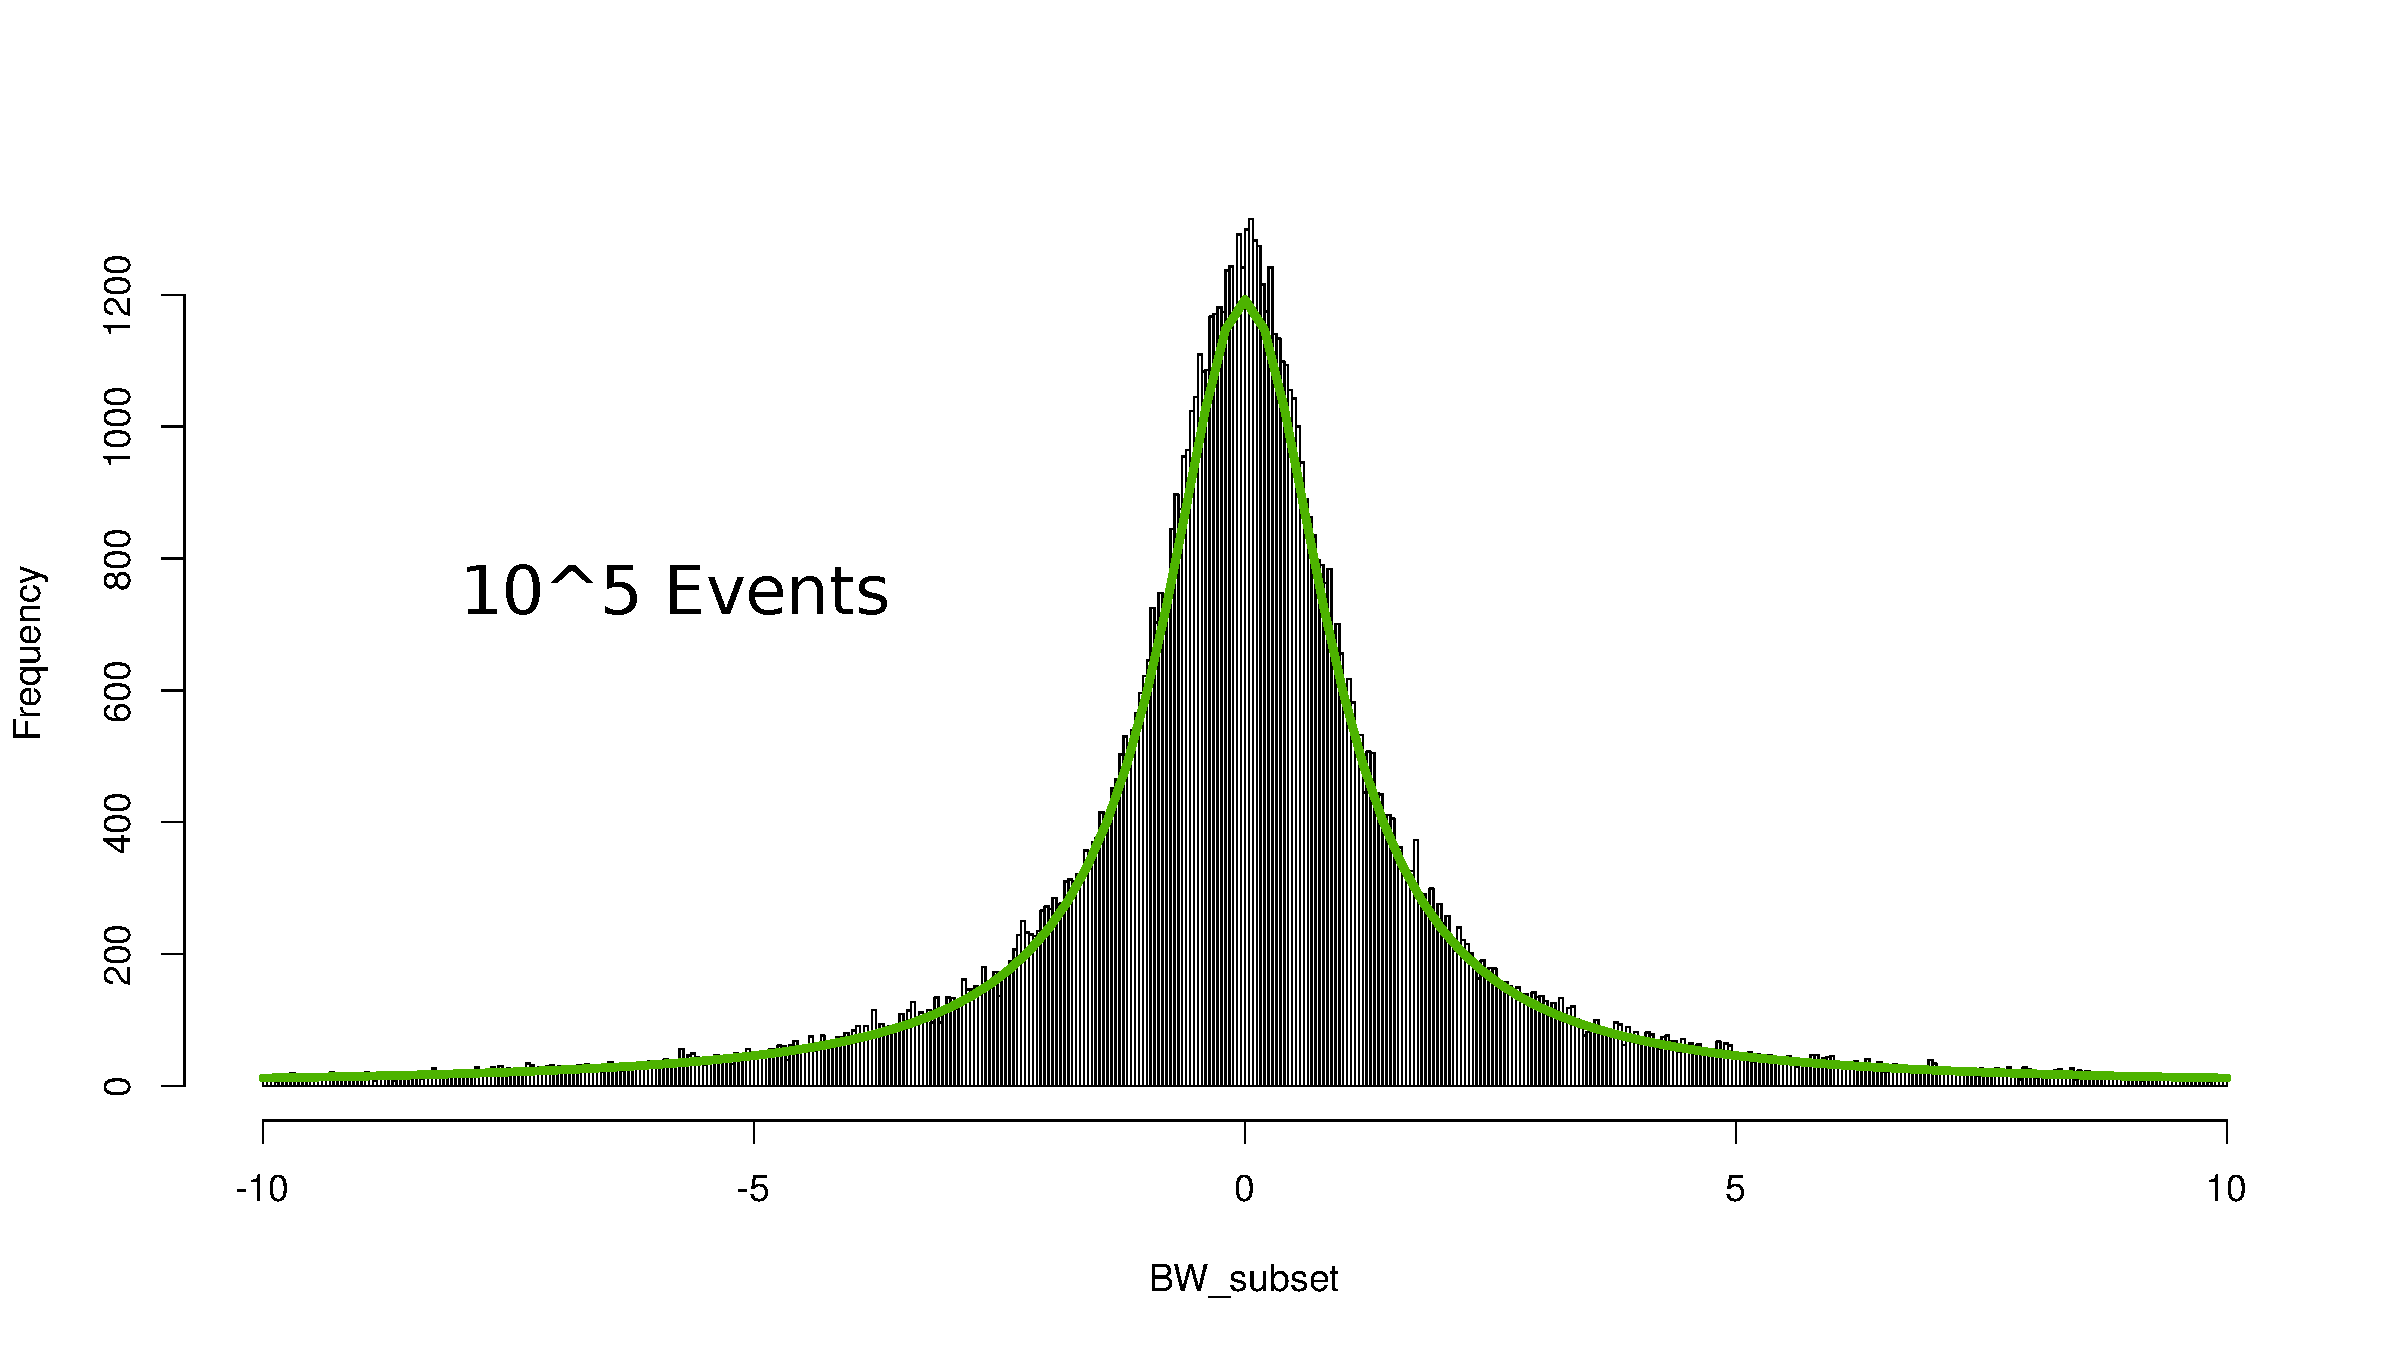
\includegraphics[width = 6in]{Immagini/BW_histogram_E5.pdf}} \\
	\subfloat[]{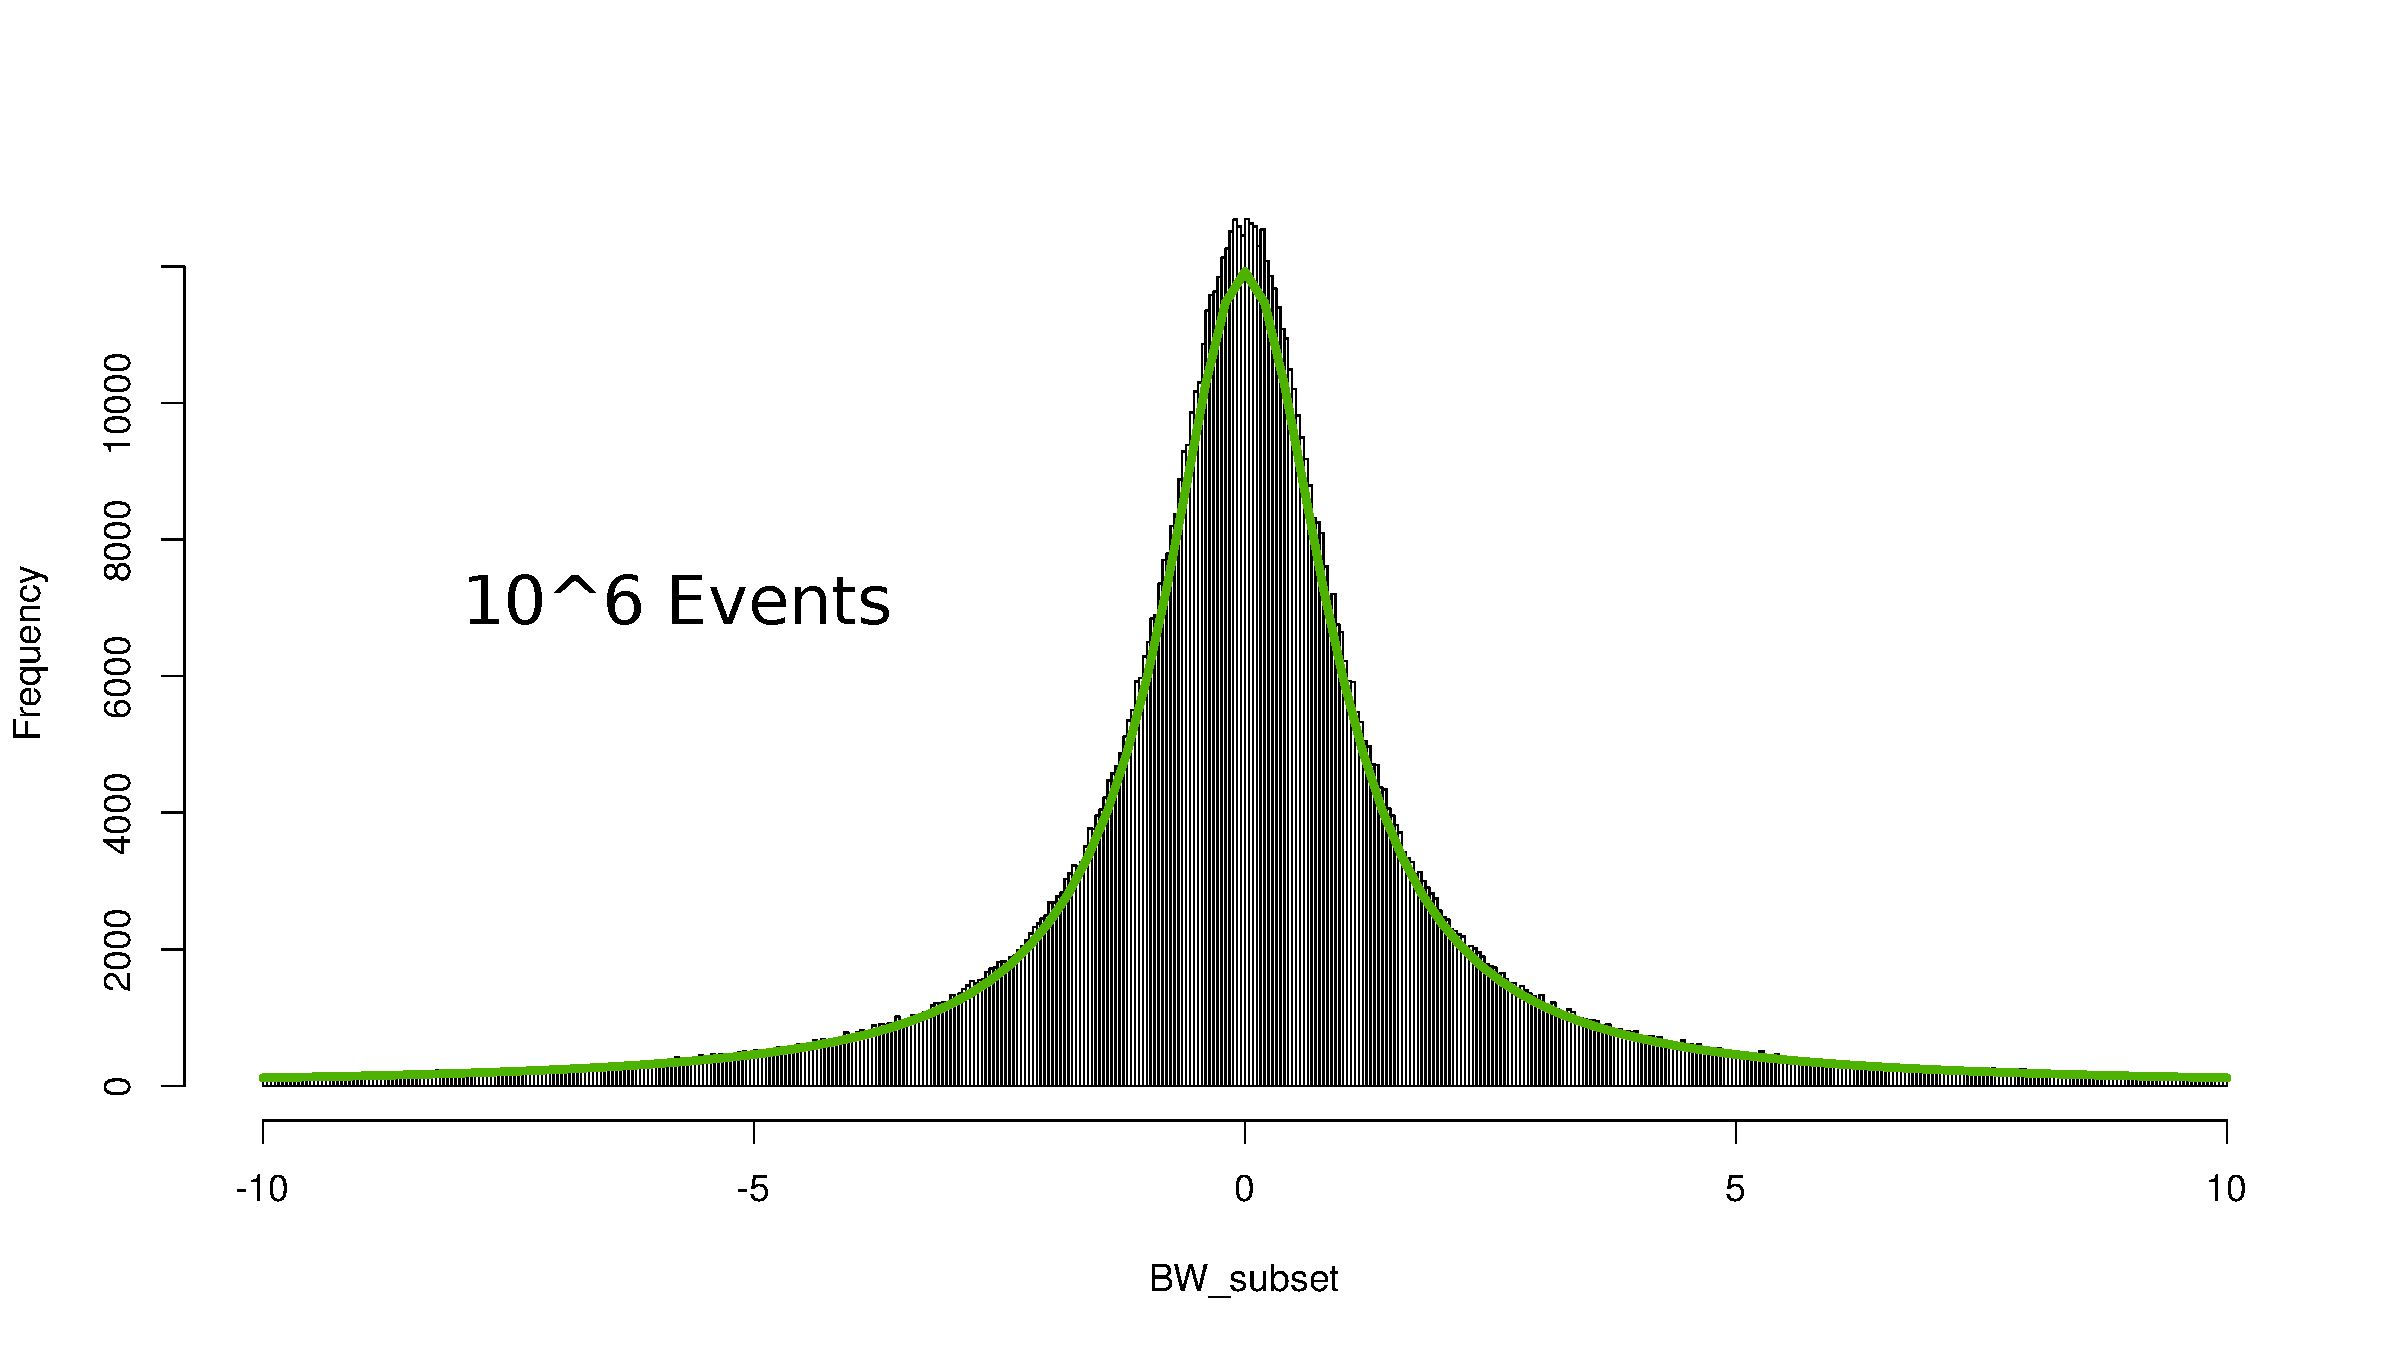
\includegraphics[width = 6in]{Immagini/BW_histogram_E6.pdf}}
	\label{fig:Breit-WIgner_N}
\end{figure}

\newpage

\noindent Passiamo adesso al problema dell'implementazione e del test di un generatore casuale uniforme. L'algoritmo che adotteremo è ad oggi considerato lo standard minimo in termini di prestazioni della sequenza pseudo-random generata: si tratta del \emph{Linear Congruential Method}, nella formulazione di Lewis, Goodman e Miller (Minimal Standard LCG).\footnote{Si vedano ad esempio le \emph{lecture notes}: \url{https://people.smp.uq.edu.au/DirkKroese/mccourse.pdf}.}\\

\vfill

\noindent In sostanza si tratta di generare la sequenza secondo la seguente formula ricorsiva:

\begin{align*}
X&_0 = s\\
X&_{t+1} = (aX_t + b) \mathop{\mathrm{mod}}c\\
U&_{t} = \frac{r}{c} \cdot X_t
\end{align*}

\noindent dove $a$, $b$, $c$ e $s$, sono numeri interi tali che

$$ a, b, s \in \{0, 1, \dots, c-1\},$$

\noindent e i numeri $\{U\}$ così costruiti risultano distribuiti uniformemente nell'intervallo aperto\footnote{Le ragioni per cui tutti i generatori di numeri pseudo-casuali lavorano su intervalli aperti sono di natura computazionale. In sostanza se qualcuno degli $U$ assumesse esattamente uno dei valori estremi si dovrebbero affrontare fastidiosi problemi numerici nell'implementazione di gran parte degli algoritmi che fanno uso di tali generatori.} $]0,r[$. Si ricordi che il risultato dell'operazione binaria $q\mathop{\mathrm{mod}}d$ è il resto della divisione di $q$ per $d$.\\

\vfill

\noindent In generale la qualità della sequenza generata dipende dai valori assegnati ai vari parametri (escluso il \emph{"seme"} $s$), e i dettagli comportano un notevole livello di complicazione matematica.\\

\vfill

\noindent  La scelta del Minimal Standard LCG

\begin{align*}
a &= 7^5\\
b &= 0\\
c &= 2^{31}-1\\
\end{align*}

\noindent pur garantendo buone proprietà di indipendenza alla sequenza $\{U\}$, risulta in un periodo di sole $(2^{31}-2)$ iterazioni, ormai inadeguato per molte applicazioni d'interesse. L'adozione qui di questo metodo è dunque motivata dalla sola semplicità di implementazione dell'algoritmo.\\

\vfill

\noindent La possibilità di scegliere semi diversi per diverse simulazioni è molto importante perché permette di ottenere sequenze indipendenti e quindi di combinare statisticamente i risultati ottenuti.\footnote{Nei metodi Montecarlo applicati alla fisica statistica, ad esempio, risulta spesso più utile combinare più simulazioni con sequenze "relativamente brevi" che generare una sola sequenza complessiva. Ciò è dovuto ai processi di minimizzazione coinvolti, che rischiano di rimanere "intrappolati" in minimi locali delle funzioni considerate. Si consulti ad esempio \href{https://www.elsevier.com/books/understanding-molecular-simulation/frenkel/978-0-12-267351-1}{\textsl{"Understanding Molecular Simulation"}} di Frenkel e Smit (Elsevier 2001).} Nel nostro caso tuttavia ci limiteremo a produrre una sola sequenza, impostando $s=1$: la sequenza risultante è riportata in Figura~\ref{fig:LCGhist} sottoforma di istogramma delle frequenze dei primi $10^5$ numeri generati.\\

\vfill

\begin{figure}
	\centering
	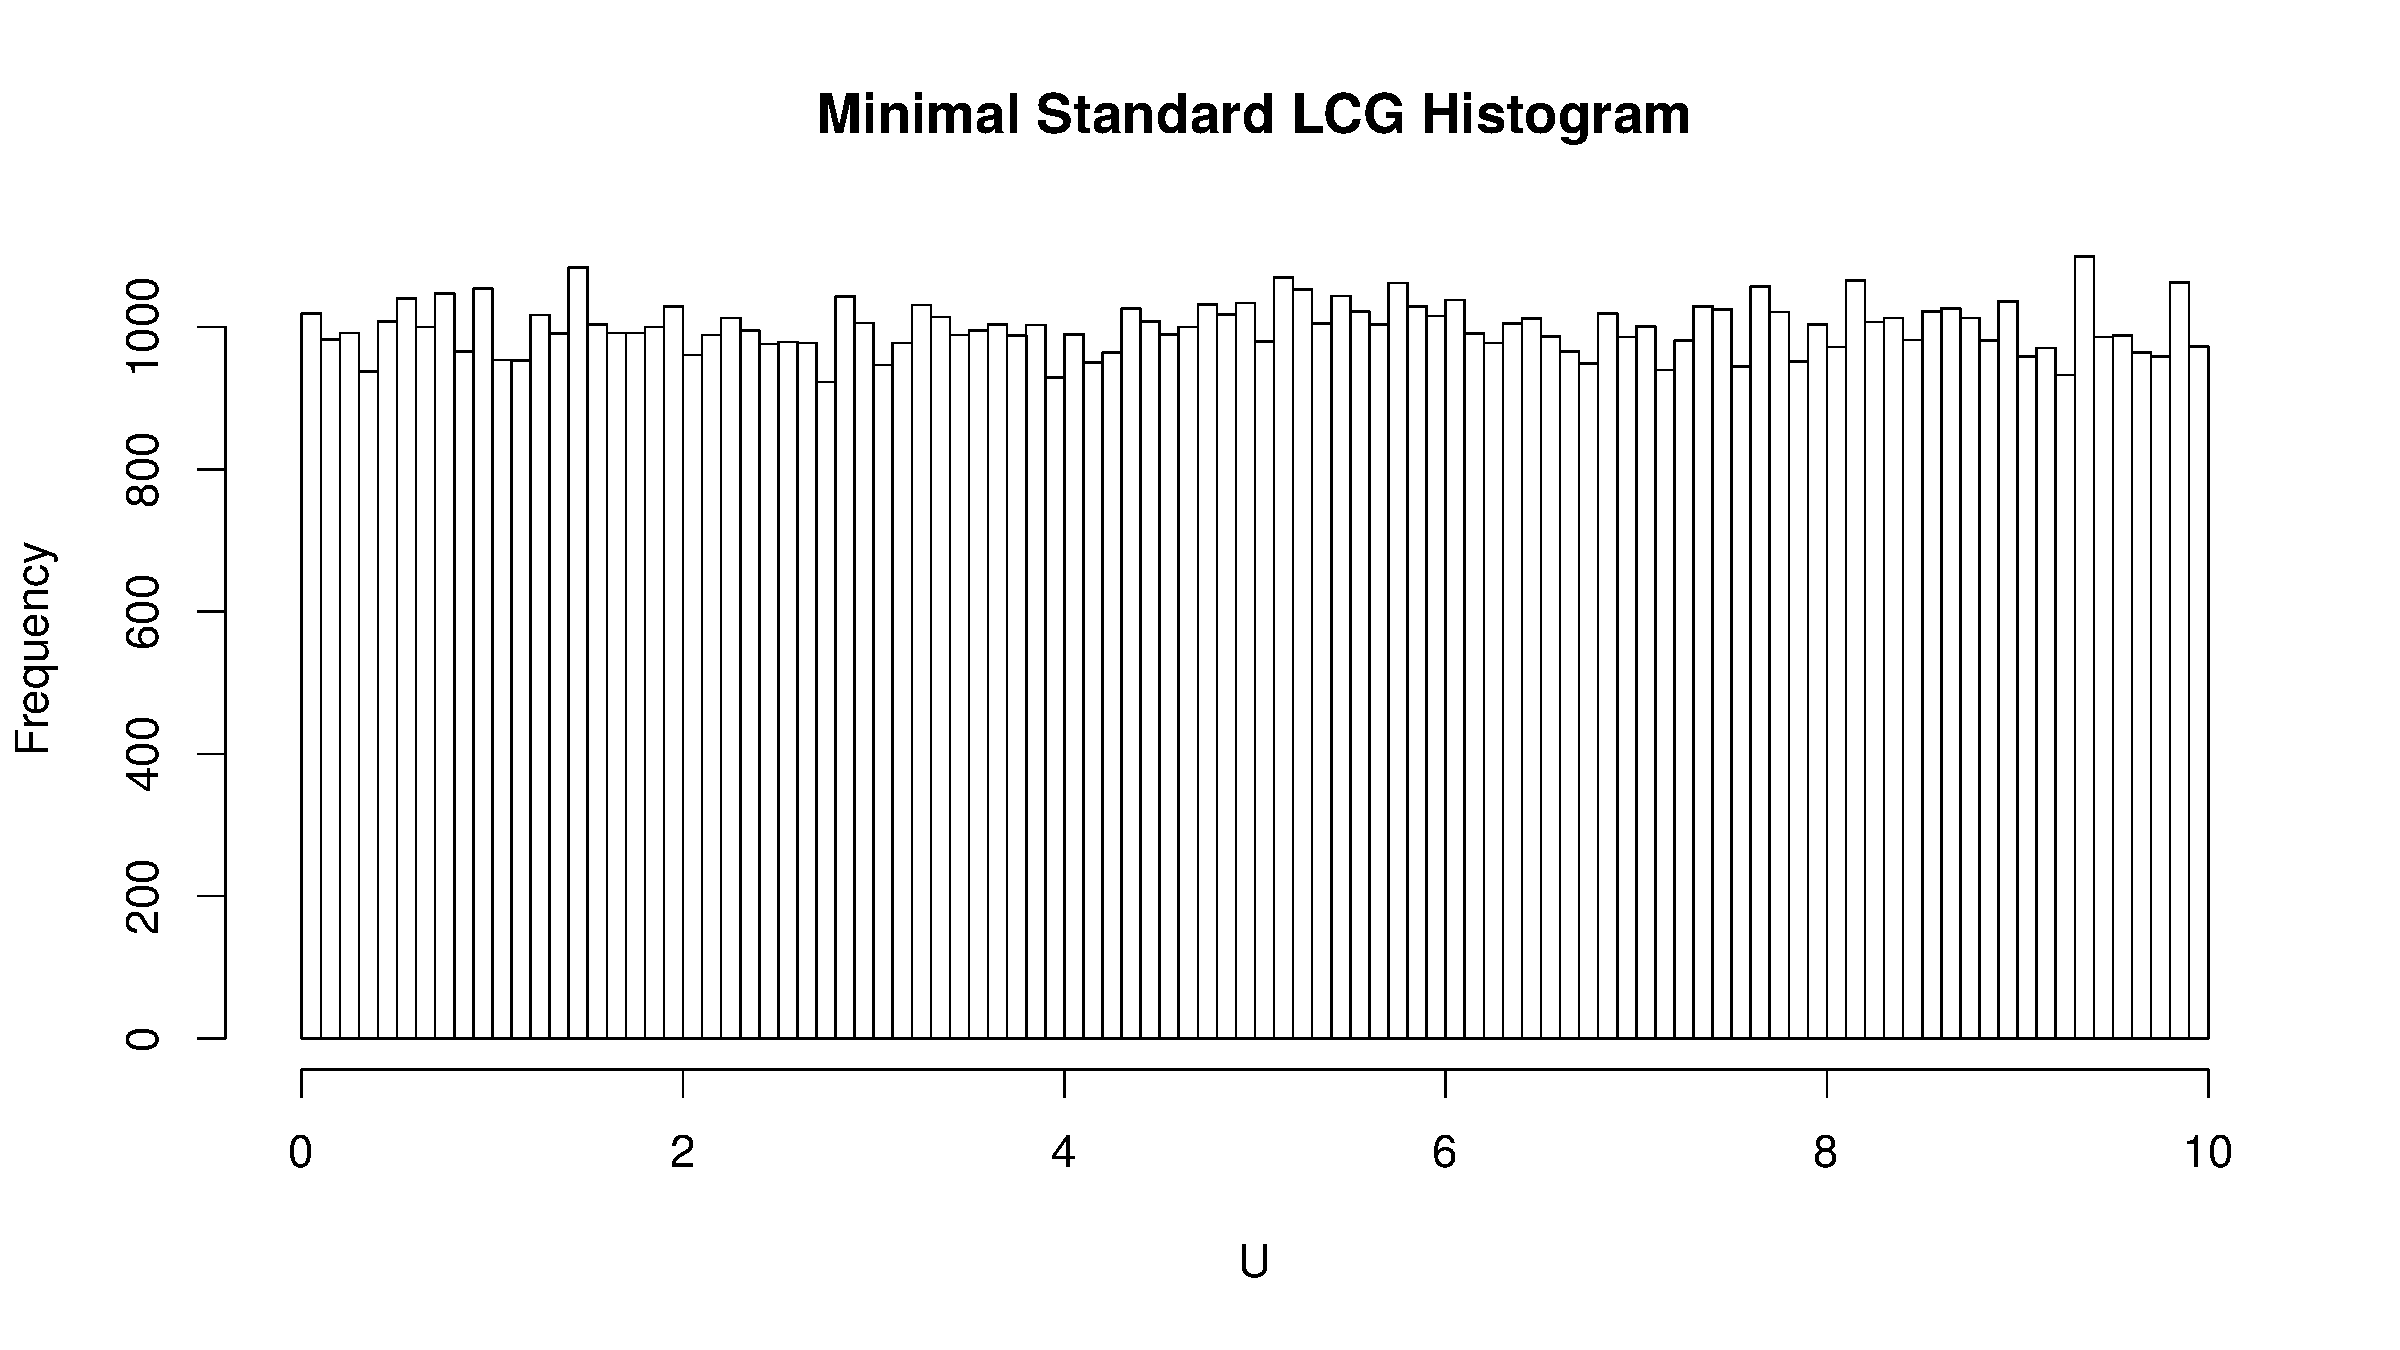
\includegraphics[width=\textwidth, trim={0 3cm 0 0}, clip]{Immagini/LCG_histogram.pdf}
	\caption{Istogramma di $10^5$ numeri generati con algoritmo Minimal Standard LCG, nell'intervallo $]0,10[$.}
	\label{fig:LCGhist}
\end{figure}

\newpage

\begin{lstlisting}[language=R, style=Rstyle, caption=\texttt{R} code for Minimal Standard LCG, xleftmargin=.02\textwidth]
# Defining Minimal Standard parameters for LCG
a = 7^5
b = 0
c = 2^31-1

# Entering user's choice parameters (length of sequence, interval radius and seed)
n = 10^5
r = 10
s = 1
	
# Inizializing recursive vectors
x = numeric(length = n)
u = numeric(length = n)
x[1] = s

# Recursive cycle
t = 1
while(t < n)
{		u[t] = x[t] * r/c; 						#Normalizing the output
		x[t+1] = (a*x[t] + b) %% c;		#Recursive action (%% is R syntax for mod)
		t = t+1
};  u[t] = x[t] * r/c 
	
# Saving a histogram plot of {u}
cairo_pdf('LCG_histogram.pdf', width = 16, height = 9, pointsize = 22)
LCG_hist = hist(u, breaks = n/1000)
LCG_hist$name = 'Minimal Standard LCG Histogram'
LCG_hist$ylab = 'Frequency'
plot(LCG_hist,  ylab=LCG_hist$ylab, main=LCG_hist$name)
dev.off()
\end{lstlisting}

\bigskip

\noindent Il primo test cui possiamo sottoporre i numeri pseudo-casuali appena generati è senz'altro un calcolo della media e della varianza campionarie. Questi sono difatti degli stimatori non distorti per cui ci aspettiamo che,  al crescere del numero di estrazioni, convergano ai "valori veri" della distribuzione di probabilità che si vuole simulare.\\

\noindent Cominciamo dunque ricordando le espressioni che definiscono la media e la varianza di una distribuzione uniforme nell'intervallo $[x,y]$:

\begin{align*}
\mathrm{E}[u(x,y)] =  \frac{x+y}{2} &=: \mu(x,y)\\ \\
\mathrm{Var}[u(x,y)] = \frac{(y-x)^2}{12} &=: \sigma^2(x,y)\\
\end{align*}

\noindent per cui nel nostro caso $\mu(0,10)=5$ e $\sigma(0,10) = 8.\bar{3}$ saranno i valori di riferimento.\\

\noindent Per quanto riguarda gli stimatori campionari, essi sono definiti come segue:

\begin{align*}
\hat{\mu}(n) &:= \frac{1}{n}\sum_{t=0}^{n-1} U_t \\ \\
\hat{\sigma}^2(n) &:= \frac{1}{n-1}\sum_{t=0}^{n-1} \left(U_t - \hat{\mu}(n)\right)^2\\
\end{align*}

\noindent Dal nostro campione otteniamo risultati soddisfacenti:

\bgroup
\def\arraystretch{1.5}
\begin{center}
\begin{tabular}{l||c|c|c}
	$n=10^5$&valore vero&valore stimato&errore relativo $\!\times\,10^{-3}$\\ \hline
	media&$5$&$5.002841\dots$&$0.568\dots $\\
	varianza&$8.\bar{3}$&$8.319576\dots$&$1.651\dots$\\	
\end{tabular}
\end{center}
\egroup

\noindent da cui deduciamo che il generatore riproduce bene tali proprietà della distribuzione uniforme.\\

\begin{lstlisting}[language=R, style=Rstyle, caption= \texttt{R} code for computing non-biased variance and mean predictors, xleftmargin=.02\textwidth]
# Assuming to have a vector u[t], with t = 1,...,n and uniform distributed in [0,r]

	# Sample Mean
	sm = 0
	for (t in seq(1, n, by = 1))
		{ sm = sm + u[t] / n }
	
	# Sample Variance
	ss = 0
	for (t in seq(1, n, by = 1))
		{ ss = ss + (u[t] - sm)^2 / (n-1) }
		
	# Displaying results and relative deviation from 'true values'
	true_media = r/2;		true_varianza = r^2/12;
	media = sm;		varianza = ss
	e_media = abs(media - true_media)/true_media
	e_varianza = abs(varianza - true_varianza)/true_varianza
	media; varianza; e_media; e_varianza;
\end{lstlisting}

\noindent Tuttavia il controllo delle sole media e varianza campionarie non può davvero garantire la bontà di una realizzazione campionaria della densità da simulare. Procederemo dunque alla costruzione di opportuni \emph{test d'ipotesi} le cui ipotesi nulle consistano nell'assumere che la sequenza generata segua effettivamente la distribuzione desiderata. Qualora i \emph{p-value} ottenuti consentano di rifiutare tale ipotesi potremmo dire di aver rilevato un problema statisticamente significativo nella sequenza generata.

\begin{description}\label{PearsonTest}
	\item[\quad\quad\! Test "chi-quadro" alla Pearson]\quad\\
	\noindent Il primo test considerato è basato sulla cosiddetta statistica \emph{"chi-quadro"}, definita come:
	
	\begin{equation*}
	\chi_{_{k-1}}^2 = \sum_{i=1}^{k} \frac{(o_i - e_i)^2}{e_i},
	\end{equation*}
	
	\noindent dove $o_i$ e $e_i$ sono le frequenze rispettivamente osservata e attesa per l'evento $E_i$, e $k-1$ sono detti essere i \emph{gradi di libertà} della statistica. Dunque nel nostro caso, diviso l'intervallo $]0,10[$ in $k$ bin, valuteremo lo scarto quadratico normalizzato tra le frequenze istogrammate dalla sequenza generata e il valore atteso di $(10^5 / k)$ eventi su ciascun bin. Evidentemente quanto più la sequenza estratta sarà aderente alla distribuzione uniforme, tanto più il valore ottenuto per la statistica $\chi^2$ sarà tendente a zero. Tra i vari test che possono essere implementati su tale statistica utilizzeremo quello di \emph{Pearson}, nativamente incorporato in \texttt{R}\footnote{Comando \texttt{chisq.test}: \url{https://stat.ethz.ch/R-manual/R-devel/library/stats/html/chisq.test.html}}, e ben adatto al caso in analisi\footnote{Il test di Pearson presenta problemi qualora alcune delle frequenze attese siano molto piccole, per cui per distribuzioni con "lunghe code" potrebbe risultare inutilizzabile. Di certo una densità uniforme non presenta criticità in tal senso.}.\smallskip

	\noindent Lavorando con tre diversi istogrammi dei nostri $10^5$ campioni abbiamo ottenuto i seguenti risultati:
	
	\bgroup
	\def\arraystretch{1.5}
	\begin{center}
		\begin{tabular}{c|c}
			Number of bins & Pearson's \emph{p-value}\\ \hline\hline
			500 & 0.94475363037911164\\
			750 & 0.86939873721667693\\
			1000 & 0.85937070391061714\\
		\end{tabular}
	\end{center}
	\egroup
	
	\noindent I \emph{p-value} ottenuti sono tali per cui fissato un qualsiasi grado ragionevole di significatività non possiamo rigettare l'ipotesi di una sequenza distribuita uniformemente: il generatore implementato ha superato il test di Pearson.
	
	\item[\quad\quad\! Test di Kolmogorov-Smirnov]\quad\\
	\noindent Un altro test d'ipotesi appropriato alla nostra situazione è quello di Kolmogorv e Smirnov (KS), basato sulla funzione cumulante $F(x)$. L'ipotesi nulla sarà dunque formulata in termini di $F(x)$ e della sua candidata realizzazione campionaria $\hat{F}_n(x)$: $H_0 = \{\hat{F}_n(x) = F(x), \,\forall x\}$. Il test è ben definito solo se $F(x)$ è continua su tutto il dominio.
	La statistica di riferimento è molto semplice: si tratta dello scarto massimo tra cumulante teorica e sua realizzazione campionaria $D_n = \max |\hat{F}_n(x) - F(x)|$, sul cui valore viene stabilito un \emph{decision boundary} oltre il quale rifiutare $H_0$. A tale valore di taglio è associata una significatività $\alpha$, secondo le formule:
	
	\begin{align*}
	D_n^{^\mathrm{cut}} &= \frac{\lambda_\alpha}{\sqrt{n}},\\
	1-\alpha &= \sum_{k=-\infty}^{\infty} (-1)^k \exp\left[-2k^2\lambda_\alpha\right].
	\end{align*}
	
	\noindent Anche il test KS è nativamente implementato in \texttt{R}\footnote{Comando \texttt{ks.test}: \url{https://stat.ethz.ch/R-manual/R-devel/library/stats/html/ks.test.html}} e per i primi 100 numeri della sequenza generata ha restituito: $D_{100} \simeq 0.05954$ e $\lambda_{0.01} \simeq 1.6276$. Dunque avendo $D_{100} < D_{100}^{^\mathrm{cut}} = 0.16276$ possiamo affermare che, fissata una significatività del 1\%, anche il test KS conferma la bontà dal nostro generatore LCG.

\end{description}

\noindent Infine osserviamo che sebbene il superamento dei test d'ipotesi proposti dia una conferma molto solida su quanto la sequenza generata riproduca la distribuzione da simulare, resta ancora la possibilità che una sequenza palesemente deterministica, e quindi affetta da spiacevoli correlazioni, minimizzi molto efficientemente gli scarti sulla $f(x)$ e sulla $F(x)$ che i test vanno a controllare. Per scongiurare questa possibilità si potrebbero ripetere i test molte volte, variando in un grande range la dimensione dei bin utilizzati, ma questo evidentemente implica un grande dispendio di risorse computazionali. Quindi preferiamo affidarci ad un metodo di controllo visivo e immediato per scovare eventuali correlazioni fra coppie di numeri estratti consecutivamente\footnote{Va da sé che andrebbero controllate anche le correlazioni fra numeri estratti non consecutivamente, ma ci aspettiamo che gli effetti di correlazione diminuiscano fortemente al crescere del numero di "passi" che ne separano l'estrazione nell'algoritmo del generatore (purché si stia ben sotto il periodo di ricorrenza!).}: costruiamo uno \emph{scatter-plot} bidimensionale in cui in ascissa sono riportati i numeri estratti ai passi dispari e in ordinata i numeri estratti ai passi pari. Il risultato, visibile in \figurename~\ref{fig:SimulatedWhiteNoise}, non mostra nessun evidente pattern distinguibile da un generico e omogeneo "rumore bianco", per cui possiamo concludere che il generatore non presenta problemi di eccessiva correlazione nella sequenza~prodotta.

\begin{figure}[h!]
	\centering
	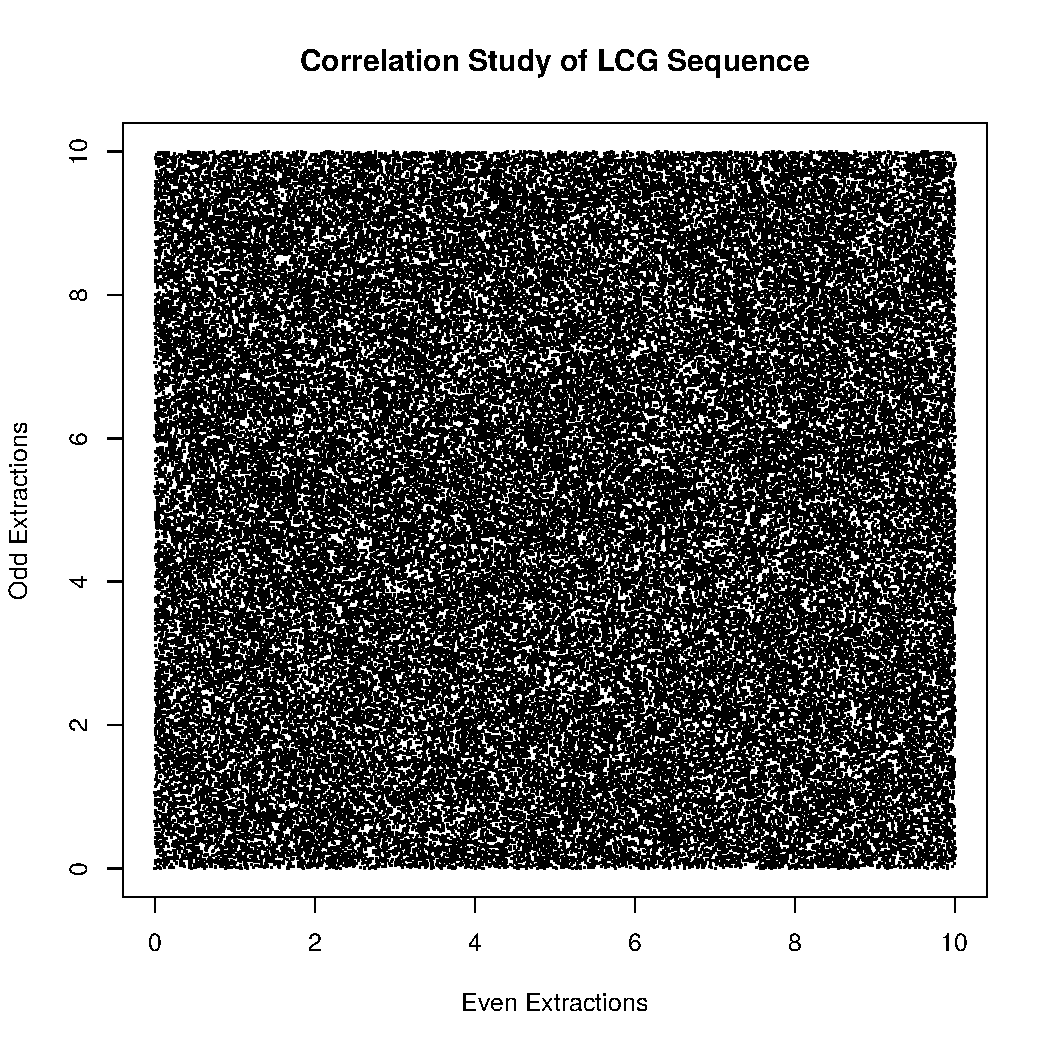
\includegraphics[width=0.55\linewidth, trim={0 0.5cm 0 0cm}, clip]{Immagini/CorrelationStudy}
	\caption{Visualizzazione delle eventuali correlazioni fra numeri estratti consecutivamente dal generatore LCG.}
	\label{fig:SimulatedWhiteNoise}
\end{figure}


\begin{lstlisting}[language=R, style=Rstyle, caption= \texttt{R} code for correlation-study of LCG random sequence]
# Assuming to have a vector u[t], of uniform distributed pseudo-random numbers...
	
	# Subset of "even extrations"
	X = u[c(TRUE,FALSE)] 
	# Subset of "odd extractions"
	Y = u[c(FALSE,TRUE)]
	# Saving a scatter-plot of Y vs X
	cairo_pdf('CorrelationStudy.pdf')
	Xlab = 'Even Extractions'
	Ylab = 'Odd Extractions'
	Title = 'Correlation Study of LCG Sequence'
	plot(X , Y, pch = '.', xlab = Xlab, ylab = Ylab, main = Title)
	dev.off()
\end{lstlisting}

\newpage
\section{Esercizio 2}

Si implementi un programma per il calcolo della costante di Eulero-Mascheroni, definita per mezzo dell'Eq.(\ref{eq:Eulero-Mascheroni}), discutendo l'influenza degli errori di calcolo sul risultato ottenuto. 

\begin{equation}
\gamma = \lim_{n \to\infty}\Biggl(\sum_{k=1}^{n}\frac{1}{k} - \log n\Biggr)
\label{eq:Eulero-Mascheroni}
\end{equation}

\[* * * \] %\smallskip

\noindent Ad un primo sguardo il problema principale del calcolo appare insito nella somma del numero armonico:

$$H_n = \sum_{k=1}^{n}\frac{1}{k}.$$

\noindent Difatti, come per qualsiasi somma in cui i termini decrescano progressivamente, è necessario implementare alcune accortezze per scongiurare il rischio di errori di troncamento (\emph{round-off}). In particolare sommando, come da implementazione letterale della definizione, i termini in ordine decrescente si rischia dopo un alto numero di iterazioni di trovarsi a sommare numeri di ordini di grandezza decisamente diversi: da un lato una somma parziale ormai "grande" e dall'altro un $k$-esimo termine via via sempre più "piccolo". Pur utilizzando variabili \emph{floating point} con precisione doppia\footnote{Opzione di default del linguaggio \texttt{R}.} ciò comporta, per $n$ sufficientemente grande, il troncamento di cifre significative dell'addendo minore e, sebbene su una singola operazione tale arrotondamento sia in genere quantitativamente accettabile, nell'iterazione di più somme può portare a risultati completamente errati.\footnote{In ultima analisi tutto dipende da quanto velocemente "decade" la coda della somma.}\\
La situazione può essere migliorata con la semplice inversione dell'ordine di somma: iniziando dai termini di ordine minimo la somma parziale crescerà molto lentamente, il tutto a fronte di addendi man mano sempre più grandi. Risulta dunque decisamente più improbabile trascurare termini a causa dei limiti di rappresentazione del calcolatore. \\

\noindent La rilevanza dell'ordine di somma è stata verificata calcolando la somma per $n=50$ con entrambi gli algoritmi e confrontando i risultati con il valore che \texttt{Wolfram-Alpha}\footnote{\url{https://www.wolframalpha.com}} riporta per $H_{50}$. Di seguito si riportano il codice utilizzato e i risultati relativi.\\

\begin{lstlisting}[language=R, style=Rstyle, caption= \texttt{R} code for summing harmonic numbers, xleftmargin=.02\textwidth]
# Entering the desired order for the harmonic sum
n = 50

# Direct: literal transposition of sum in for cycle
H = 0
for (k in seq(1,n, by = 1))
{ H = H+ 1/k	} 
print(H, digits = 16)

# Trick: invert sum order (avoids round-offs!)
H = 0
k = n
while (k > 0)
{ H = H + 1/k; k = k - 1 }
print(H, digits = 16)
\end{lstlisting}

\bgroup
\def\arraystretch{2}
\begin{center}
	\begin{tabular}{l||c}
		\texttt{Wolfram-Alpha} [ 16 digits ]&$H_{50} \simeq 4.49920533832942\mathbf{\check{5}}$ \\  \hline
		Direct algorithm [ 16 digits ]&$H_{50} \simeq 4.49920533832942\mathbf{\check{3}}$ \\ 
		Inverted sum [ 16 digits ]&$H_{50} \simeq4.49920533832942\mathbf{\check{5}}$ \\ 
	\end{tabular}
\end{center}
\egroup

\noindent Il vantaggio ottenuto con l'inversione dell'ordine degli addendi permette di guadagnare una cifra significativa rispetto all'implementazione diretta della somma, come risulta evidente osservando in tabella le cifre evidenziate. \\

\noindent Tuttavia implementando di conseguenza il calcolo di $\gamma$ osserviamo degli errori che limitano ancora severamente la precisione ottenibile: nonostante la somma invertita dia un risultato più piccolo dell'algoritmo diretto (e quindi più vicino al valore vero, che li minora entrambi) non riusciamo in nessuno dei due casi a fissare più di quattro cifre significative. 

\bgroup
\def\arraystretch{2}
\begin{center}
	\begin{tabular}{l||c|c}
		"True value" [ First 16 digits from \href{https://oeis.org/A001620}{\texttt{O.E.I.S.}}] &$\gamma \simeq 0.5772\mathbf{\check{1}}56649015329$  &$|\gamma_{_\mathrm{true}}  - \gamma_{_\mathrm{calc.}} |$ [ 1 digit ]\\  \hline
		Direct algorithm [ $n=10^5$ | 16 digits ]&$\gamma \simeq 0.5772\mathbf{\check{2}}06648932138$ & 5e-06 \\ 
		Inverted sum [ $n=10^5$ | 16 digits ]&$\gamma \simeq0.5772\mathbf{\check{2}}06648931792$ & 5e-06\\ 
	\end{tabular}
\end{center}
\egroup

\begin{lstlisting}[language=R, style=Rstyle, caption= \texttt{R} code for naïve computation of Eulero-Mascheroni constant, xleftmargin=.02\textwidth]
# Setting Eulero-Mascheroni constant (correct up to 16 digits)
EM = 0.5772156649015329

# Entering the desired truncation-parameter for the series
n = 10^5

# First attempt: direct algorithm from definition
em = -log(n)
for (k in seq(1,n, by = 1))
{ em = em + 1/k	} 
print(EM, digits = 16)
print(em, digits = 16)
print(abs(EM-em), digits = 1)

# Second attempt: inverted sum order
em = 0
k = n
while (k > 0)
{ em = em + 1/k; k = k - 1 }
em = em-log(n)
print(EM, digits = 16)
print(em, digits = 16)
print(abs(EM-em), digits = 1)
[...
\end{lstlisting}

\noindent Tornando all'equazione (\ref{eq:Eulero-Mascheroni}) notiamo infatti che pur costruendo in maniera ottimizzata il numero armonico $H_n$, sottraendogli "tutto insieme" il logaritmo di $n$ ci si ritrova ancora in una situazione spiacevole: si stanno sostanzialmente sottraendo tra loro due numeri "grandi" - dello stesso ordine in $n$ - allo scopo di ottenere un risultato dell'ordine dell'unità e quindi certamente svariati ordini di grandezza sotto $n$; ne consegue che per le cifre significative del risultato utilizziamo solo una piccola parte dei \emph{bit} di rappresentazione disponibili.\\

\noindent Per risolvere il problema l'idea è quindi di scomporre in addendi anche il logaritmo di $n$ in modo da costruire $\gamma$ sommando (algebricamente) termini il più possibile confrontabili con la somma parziale. Sebbene la successione logaritmica non abbia uno sviluppo in serie immediato, è possibile raggiungere l'obiettivo auspicato con delle opportune manipolazioni:\\ \bigskip

Definendo la successione

\begin{equation*}
\gamma_n =  H_n - \log n,\\
\end{equation*}

possiamo scrivere

\begin{align*}
\gamma_n &= H_n - k \frac{\log n}{k}\quad\forall k > 0  \\
&=  H_n - \frac{\log n^k}{k}\\
&= H_n - \frac{H_{n^k} - \gamma_{n^k}}{k}\,\, \Longleftrightarrow\,\,\gamma_n - \frac{\gamma_{n^k}}{k} =  H_n - \frac{H_{n^k}}{k},\\
\end{align*}

per cui, dal momento che $\displaystyle\lim_{n \to\infty}\gamma_n\equiv \displaystyle\lim_{n \to\infty}\gamma_{n^k} = \gamma$, si ha $\gamma = \displaystyle\frac{k}{k-1}\lim_{n \to\infty}\left(H_n - \frac{H_{n^k}}{k}\right)$.\\

Scegliendo in particolare $k=2$ otteniamo una semplice formula, dovuta al matematico russo Mačys\footnote{\href{https://doi.org/10.4213/mzm9386}{J. J. Mačys, \emph{On the Euler–Mascheroni Constant}, Mat. Zametki, 94:5 (2013), 695–701 \emph{or} Math. Notes, 94:5 (2013), 647–652 }}:


\begin{align}
\gamma &= \lim_{n \to\infty}\left(2H_n - H_{n^2}\right)\nonumber\\
&= \lim_{n \to\infty}\left(1 +\frac{1}{2} + \dots + \frac{1}{n} - \frac{1}{n+1} - \dots - \frac{1}{n^2}\right).
\end{align}\bigskip

\noindent La formula di Mačys ben si presta ad un'implementazione analoga a quella utilizzata per il calcolo ottimizzato del numero armonico $H_n$ e ci permette di abbassare di più di cinque ordini di grandezza l'errore $|\gamma_{_\mathrm{true}}  - \gamma_{_\mathrm{calc.}} |$ - da circa $5\cdot10^{-6}$ a circa $10^{-11}$ - portando fino a nove le cifre significative corrette:

\begin{align*}
\gamma_{_\mathrm{true}}  &= 0.577215664\mathbf{\check{9}}015329\dots\\
\gamma_{_\mathrm{Macys}} &\simeq 0.577215664\mathbf{\check{8}}885598\dots\\
\end{align*}

\noindent Infine la formula di Mačys può essere resa più accurata valutando l'errore commesso troncando a $n$ finiti per mezzo di sviluppi asintotici del numero armonico $H_n$. Senza riportarne esplicitamente la derivazione utilizziamo la correzione\footnote{Maggiori dettagli possono essere trovati consultando la seguente discussione (\href{https://math.stackexchange.com/questions/129777/what-is-the-fastest-most-efficient-algorithm-for-estimating-eulers-constant-g}{link}) sul forum \texttt{math.stackexchange.com}}

\begin{align}
\gamma &=  \lim_{n \to\infty}\left(1 +\frac{1}{2} + \dots + \frac{1}{n} - \frac{1}{n+1} - \dots - \frac{1}{n^2} \underbracket{-\frac{1}{n^2 + 1} - \dots - \frac{1}{n^2 + n}}_{\text{1st Trick}} \overbracket{+\frac{1}{6n^2} - \frac{1}{6n^3}}^{\text{2nd Trick}}\right)\\
&= \lim_{n \to\infty}\left(2H_n - H_{n(n+1)} + \frac{1}{6n^2} - \frac{1}{6n^3}\right),\nonumber
\end{align}

\noindent il cui errore per $n$ finito può essere dimostrato essere dell'ordine $\mathop{O}(n^{-4})$.\\

\noindent Ne risulta il guadagno di altre due cifre significative corrette, con un errore assoluto di circa $4\cdot10^{-12}$. Notiamo subito che tale valore è molto maggiore di $n^{-4} = 10^{-20}$, segno che la precisione è ancora limitata da errori di troncamento sulle singole somme. Tuttavia il lavoro di ottimizzazione dell'algoritmo ha permesso complessivamente di abbattere di ben sei ordini di grandezza l'errore sul calcolo, rispetto all'implementazione pedissequa della formula (\ref{eq:Eulero-Mascheroni}). In ragione di ciò riteniamo il risultato ottenuto pienamente soddisfacente.\\

\noindent In conclusione riportiamo una tabella comparativa dei risultati relativi ai quattro algoritmi utilizzati e a seguire il codice per l'implementazione delle formule di Mačys.\\

\bgroup
\def\arraystretch{2}
\begin{center}
	\begin{tabular}{l||c|c}
		"True value" [ First 16 digits from \href{https://oeis.org/A001620}{\texttt{O.E.I.S.}}] &$\gamma \simeq 0.5772156649015329$  &$|\gamma_{_\mathrm{true}}  - \gamma_{_\mathrm{calc.}} |$ [ 1 digit ]\\  \hline
		Direct algorithm [ $n=10^5$ | 16 digits ]&$\gamma \simeq 0.5772\mathbf{\check{2}}06648932138$ & 5e-06 \\ 
		Inverted sum [ $n=10^5$ | 16 digits ]&$\gamma \simeq0.5772\mathbf{\check{2}}06648931792$ & 5e-06\\ 
		Mačys Formula [ $n=10^5$ | 16 digits ]&$\gamma\simeq0.577215664\mathbf{\check{8}}885598$ & 1e-11\\
		Mačys $+$ Tricks [ $n=10^5$ | 16 digits ]&$\gamma\simeq0.57721566490\mathbf{\check{5}}2262$ & 4e-12\\
	\end{tabular}
\end{center}
\egroup

\bigskip

\begin{lstlisting}[language=R, style=Rstyle, caption= \texttt{R} code for efficient computation of Eulero-Mascheroni constant, xleftmargin=.02\textwidth]
...]
# Third attempt: Macys formula
em = 0
k = n^2
while (k > n)
	{ em = em - 1/k; k = k - 1 }
while (k > 0)
{ em = em + 1/k; k = k -1 }
print(EM, digits = 16)
print(em, digits = 16)
print(abs(EM-em), digits = 1)
	
# Final refinement: some magic
em = 0
k = n^2+n # 1st Trick
while (k > n)
{ em = em - 1/k; k = k - 1 }
while (k > 0)
{ em = em + 1/k; k = k - 1 }
em = em + 1/(6*n^2) - 1/(6*n^3)# 2nd Trick
print(EM, digits = 16)
print(em, digits = 16)
print(abs(EM-em), digits = 1)
\end{lstlisting}

\newpage
\section{Esercizio 3}

Si scriva in un linguaggio di programmazione opportuno una procedura per la minimizzazione col metodo del simplesso e la si utilizzi per determinare il minimo globale o i minimi locali di:

\begin{itemize}
	
	\item Funzione di Easom\\
	$f(x,y) = -\cos (x) \cos (y) \exp[-(x-\pi)^2 - (y-\pi)^2]$
	
	\item Funzione di Goldstein-Price\\
	$f(x,y) = \exp[0.5(x^2+y^2-25)^2] + \sin^4(4x-3y) + 0.5(2x+y-10)^2$
	
	\item Funzione di Bukin Nr.~6\\
	$f(x,y) = 0.01\left|x+10\right| + 100\sqrt{\left|y-0.01x^2\right|}$
	
	\item Funzione di Booth\\
	$f(x,y) = (x+2y-7)^2 + (2x+y-5)^2$
	
\end{itemize}
	
\noindent discutendo i risultati ottenuti.

\vfill \[* * * \] \smallskip

\noindent Il metodo Nelder-Mead (anche detto del \emph{del simplesso} o \emph{metodo ameba}) è un algoritmo non lineare per la minimizzazione di funzioni di $n$ variabili senza l'uso delle derivate. La nozione centrale è quella di simplesso $n$-dimensionale, definito come un politopo convesso con $n+1$ vertici\footnote{Per politopo si intende la generalizzazione a $n$ qualsiasi del poligono ($n=2$) e del poliedro ($n=3$). La nozione di convessità è l'immediata estensione di quella in bassa dimensione.}.\vfill

\noindent Consideriamo una generica funzione $f\!: \mathbb{R}^n \mapsto \mathbb{R}$, sufficientemente regolare, della quale ci interessano i minimi locali e globali. L'idea di Nelder e Mead consiste nel definire un generico simplesso di prova\footnote{In realtà la scelta del primo insieme di vertici è decisiva sull'efficienza pratica del metodo, ragion per cui sarà opportuno valutarla attentamente.} e valutare tale funzione sui vertici di tale politopo. Definiti questi come $\mathbf{x}_i \in \mathbb{R}^n,\enspace i = 1\dots n+1$, si otterrà allora la sequenza di valori $\{f(\mathbf{x}_i)\}$; i vertici sono da intendersi ordinati per soddisfare $f(\mathbf{x}_1) \leq \dots \leq f(\mathbf{x}_{n+1})$. A questo punto si ipotizza euristicamente che il vertice $\mathbf{x}_{n+1}$ sia quello con minore probabilità di trovarsi in prossimità di un qualche minimo di $f(\mathbf{x})$ e si procede a valutarne un sostituto, con la speranza che quest'ultimo produca un valore inferiore rispetto al \emph{penultimo} vertice, una volta valutata in esso la funzione. Come primo tentativo si valuta dunque una \emph{riflessione} dell'ultimo vertice della sequenza rispetto al \emph{centroide} $\bar{\mathbf{x}}$ degli altri $n$ vertici, ossia:

\begin{equation*}
\mathbf{x}_\mathrm{r} = \bar{\mathbf{x}} + \mu_\mathrm{r}(\bar{\mathbf{x}}-\mathbf{x}_{n+1}), \enspace \bar{\mathbf{x}} = \frac{1}{n}\sum_{k=1}^{n} \mathbf{x}_k,\enspace \mu_\mathrm{r} > 0,
\end{equation*}

\noindent Qualora tale mossa non avesse successo, ossia se $f(\mathbf{x}_\mathrm{r} )  \geq f(\mathbf{x}_{n})$, si prova a sostituire uno degli altri punti, con una qualche riduzione del volume del simplesso. L'idea è in definitiva che il simplesso evolva per riflessioni, espansioni e contrazioni\footnote{Da qui il riferimento alle amebe!} fino ad individuare una direzione di gradiente e così raggiungere velocemente un minimo locale della funzione $f$.\vfill

\noindent Esistono vari modi per implementare un metodo del simplesso che sia concretamente robusto (e magari efficiente). L'algoritmo che noi presentiamo prevede le seguenti mosse gerarchiche:

\begin{enumerate}
	\item \emph{Ordinamento}  dei vertici secondo il valore che in essi assume la funzione obiettivo:
	
	\begin{equation*}
	f(\mathbf{x}_1) \leq \dots \leq f(\mathbf{x}_i)  \leq \dots \leq f(\mathbf{x}_{n+1}).
	\end{equation*}
	
	\item Valutazione della \emph{tolleranza} raggiunta sui valori $f(\mathbf{x}_i)$: se $\left|f(\mathbf{x}_{n+1}) - f(\mathbf{x}_1)\right| \leq \varepsilon \ll 1$ o è stato individuato un minimo o il simplesso è entrato in una regione di \emph{plaeau}; in entrambi i casi si chiude la routine. Se invece si è al di sopra della tolleranza stabilita $\varepsilon$ si prosegue con il punto successivo.
	
	\item Calcolo del \emph{centroide} $\bar{\mathbf{x}}$ dei primi $n$ vertici	e del candidato sostituto per $\mathbf{x}_{n+1}$: $\mathbf{x}_\mathrm{r} = \mathbf{x}_\mathrm{r}(\mu_\mathrm{r})$.
	
	\item \emph{Riflessione} effettiva di $\mathbf{x}_{n+1}$ in $\mathbf{x}_\mathrm{r}$ se quest'ultimo risulta migliore di  $\mathbf{x}_{n}$ ma non più valido di $\mathbf{x}_{1}$, ossia se $f(\mathbf{x}_1) \leq f(\mathbf{x}_\mathrm{r}) < f(\mathbf{x}_n)$. In tale caso si ritorna al punto 1. Altrimenti si procede con i punti seguenti.
	
	\item \emph{Espansione} del simplesso. Se il punto riflesso $\mathbf{x}_\mathrm{r}$ risulta migliore di tutti i vertici, secondo $f(\mathbf{x}_\mathrm{r}) < f(\mathbf{x}_1)$, si procede a calcolare il \emph{punto espanso} $\mathbf{x}_\mathrm{e}= \bar{\mathbf{x}} + \mu_\mathrm{e}(\bar{\mathbf{x}}-\mathbf{x}_{n+1}),\enspace \mu_\mathrm{e} > \mu_\mathrm{r}$ e a valutare in esso la funzione $f$. Se $f(\mathbf{x}_\mathrm{e}) < f(\mathbf{x}_\mathrm{r})$ vale la pena di allungare il simplesso nella direzione di riflessione fino a $\mathbf{x}_\mathrm{e}$, che dunque viene sostituito a $\mathbf{x}_{n+1}$. Se invece $f(\mathbf{x}_\mathrm{e}) > f(\mathbf{x}_\mathrm{r})$ ci si accontenta di sostituire $\mathbf{x}_\mathrm{r}$ a $\mathbf{x}_{n+1}$. In entrambi i casi si ritorna al punto 1.
	
	\item \emph{Contrazione}. Resta ancora il caso in cui $f(\mathbf{x}_\mathrm{r}) \geq f(\mathbf{x}_{n})$. In tale situazione risulta necessario contrarre la dimensione del simplesso, perché presumibilmente confinato dentro una "valle" angusta rispetto alle sue dimensioni. Distinguiamo due casi: se addirittura $f(\mathbf{x}_\mathrm{r}) \geq f(\mathbf{x}_{n+1})$ sarà necessario operare una "contrazione interna":
	
	\begin{equation*}
	\mathbf{x}_\mathrm{c}^\mathrm{int} = \bar{\mathbf{x}} + \mu_\mathrm{c}^\mathrm{int} (\bar{\mathbf{x}} - \mathbf{x}_{n+1}),\enspace -1 \leq \mu_\mathrm{c}^\mathrm{int} < 0;
	\end{equation*}
	
	se invece $f(\mathbf{x}_n) \leq f(\mathbf{x}_\mathrm{r}) < f(\mathbf{x}_{n+1})$ si può contrarre andando comunque a riflettere oltre il centroide, in una cosiddetta "contrazione esterna":
	
	\begin{equation*}
	\mathbf{x}_\mathrm{c}^\mathrm{ext} = \bar{\mathbf{x}} + \mu_\mathrm{c}^\mathrm{ext} (\bar{\mathbf{x}} - \mathbf{x}_{n+1}),\enspace 0 < \mu_\mathrm{c}^\mathrm{ext} < \mu_\mathrm{r},
	\end{equation*}
	
	ottenendo un vantaggio sulla velocità complessiva di convergenza della routine. In entrambi i casi si valuta la disuguaglianza $f(\mathbf{x}_\mathrm{c}) < f(\mathbf{x}_\mathrm{r})$: se soddisfatta si sostituisce il punto contratto a $\mathbf{x}_{n+1}$ e si torna al punto 1; altrimenti non resta altro che abbandonare la direzione individuata da $\mathbf{x}_{n+1}$ e $\bar{\mathbf{x}}$ e cercarne un'altra operando sugli altri vertici secondo il punto seguente.
	
	\item \emph{Riduzione}. Nel raro caso in cui la contrazione aumenti il valore di $f$  si procede a contrarre tutti i vertici tranne $\mathbf{x}_1$, secondo la:
	
	\begin{equation*}
	\mathbf{x}_i = \mathbf{x}_1 + \mu_\mathrm{c}^\mathrm{red}(\mathbf{x}_i - \mathbf{x}_1),\enspace\forall i \in \{2\dots n\}.
	\end{equation*}
	
	Segue invariabilmente il passo 1.
	
\end{enumerate}

\vfill

\noindent Da quel che abbiamo visto risulta che la routine prevede 5 parametri liberi, da scegliere in base alle esigenze del singolo caso. I valori più comunemente (e da noi) impiegati sono:

\begin{align*}
\mu_\mathrm{r} &= 1\quad\quad\quad\quad\mu_\mathrm{e} = 2\\
\\
\mu_\mathrm{c}^\mathrm{ext} &= 0.5\quad\quad\quad\!\!\mu_\mathrm{c}^\mathrm{int} = - 0.5\\
\\
\mu_\mathrm{c}^\mathrm{red} &= 0.5\\
\end{align*}

\vfill

\newpage

\noindent Di seguito riportiamo il codice che implementa in \texttt{Phyton} l'algoritmo appena illustrato:

\begin{lstlisting}[language=python, style=Pystyle, caption=\texttt{Python} code for Simplex Minimization Routine, label=list:Simplex, 	captionpos=b]
from pylab import *
import numpy as np
import operator

## Search-Routine Parameters
n = 2 
mu_exp = 2.0
mu_rifl = 1.0
mu_contr_ex = 1.0/2
mu_contr_int = -1.0/2
mu_red = 1.0/2

## Random Trial Simplex [may need a careful range-definition]
def vertici_iniziali():
	import random 
	random.seed()
	vertici=[]
	for in in range(n+1):
		x=random.uniform(-12,-8);
		y=random.uniform(0,3);
		vertici.append([x,y])
	return vertici 
vertex=vertici_iniziali() 
x1=vertex[0]
x2=vertex[1]
x3=vertex[2]

## Target Functions [uncomment the desired one]
def f(x,y):
	# EASOM
	#return -1.0*np.cos(x)*np.cos(y)*np.exp(-((x-np.pi)**2+(y-np.pi)**2))         
	# GOLDSTEIN-PRICE
	#return np.exp(0.5*(x**2+y**2-25)**2)+(np.sin(4*x-3*y))**4+0.5*(2*x+y-10)**2
	# BUKIN 6th   
	#return 100*abs(y-0.01*x**2)+0.01*abs(x+10)
	# BOOTH                                   
	#return  (x+2*y-7)**2+(2*x+y-5)**2
	                           
data_x=[x1,x2,x3]
data_f=[f(x1[0],x1[1]),f(x2[0],x2[1]),f(x3[0],x3[1])]
data=[[f(x1[0],x1[1]),x1],[f(x2[0],x2[1]),x2],[f(x3[0],x3[1]),x3]]
print (data)

## Ordering [increasing f(x)]
data=sorted(data,key=operator.itemgetter(0)) 
data_f= [item[0] for item in data]
data_x= [item[1] for item in data]
print (data_f, 'f(trial simplex)')
print ( data_x ,'trial simplex')

## Plotting the Target Function and the Trial Simplex
xvec = np.linspace(-12, -8, 1000)
yvec = np.linspace(-0, 3, 1000)
X,Y = np.meshgrid(xvec, yvec)
Z = f(X, Y).T
fig, ax = subplots()
im = imshow(Z, cmap=cm.magma, vmin=Z.min(), vmax=Z.max(), extent=[-12, -8, 0, 3])
im.set_interpolation('bilinear')
cb = fig.colorbar(im)
Xvertex = np.array([])
Yvertex = np.array([])
for i in range(n+1):
	Xvertex = np.append(Xvertex, data_x[i][0])
	Yvertex = np.append(Yvertex, data_x[i][1])
plt.scatter(Xvertex,Yvertex, color='green', edgecolor='black', s=200)
coord = data_x
coord.append(coord[0]) # have to repeat the first point to create a 'closed loop'
xs, ys = zip(*coord) # creates lists of x and y values
plt.plot(xs,ys, color='white', alpha=0.3, ls='--') # Polytope draws up 

## Evolving the Simplex
epsilon = 10**(-5) # See...
loop=1
while data_f[n]- data_f[0] > epsilon: # ...this!

	loop=loop+1

	## Centroid
	a=np.array(data_x[0:n])
	a=a/n
	xc=a.sum(axis=0)
	xr=(1+mu_rifl)*xc-mu_rifl*np.array(data_x[n])
	fr=f(xr[0],xr[1])
	print ( fr, 'fr')
	
	## Reflection step
	if data_f[0]<=fr<data_f[n-1]:   
		data[n][1]=xr
		data[n][0]=f(xr[0],xr[1])
		data=sorted(data,key=operator.itemgetter(0)) 
		print('loop',loop,'riflessione')
		data_f= [item[0] for item in data]
		data_x= [item[1] for item in data]
		print (data_f, 'valori funzione ')
		print ( data_x ,'vertici ')
		for i in range(n+1):
			Xvertex = np.append(Xvertex, data_x[i][0])
			Yvertex = np.append(Yvertex, data_x[i][1])
		plt.scatter(Xvertex,Yvertex, color='white', edgecolor='black')
		coord = data_x
		coord.append(coord[0]) # repeat the first point to create a 'closed loop'
		xs, ys = zip(*coord) # create lists of x and y values
		plt.plot(xs,ys, color='white', alpha=0.3, ls='--') 
		continue
	
	## Expansion step
	if fr<data_f[0]: 
		a=np.array(data_x[0:n])
		a=a/n
		xc=a.sum(axis=0)
		xe=(1+mu_exp)*xc-mu_exp*np.array(data_x[n])
		fe=f(xe[0],xe[1])
		if fe<fr: 
			data[n][1]=xe  
			data[n][0]=f(xe[0],xe[1])
			data=sorted(data,key=operator.itemgetter(0)) 
			print('loop' ,loop,'espansione')
			data_f= [item[0] for item in data]
			data_x= [item[1] for item in data]
			print (data_f, 'valori funzione ')
			print ( data_x ,'vertici ')
			for i in range(n+1):
				Xvertex = np.append(Xvertex, data_x[i][0])
				Yvertex = np.append(Yvertex, data_x[i][1])
			plt.scatter(Xvertex,Yvertex, color='white', edgecolor='black')
			coord = data_x
			coord.append(coord[0]) # repeat the first point to create a 'closed loop'
			xs, ys = zip(*coord) # create lists of x and y values
			plt.plot(xs,ys, color='white', alpha=0.3, ls='--') 
			continue 
		else: 
			data[n][1]=xr
			data[n][0]=f(xr[0],xr[1])
			data=sorted(data,key=operator.itemgetter(0))
			print('loop',loop,'riflessione')
			data_f= [item[0] for item in data]
			data_x= [item[1] for item in data]
			print (data_f, 'valori funzione ')
			print ( data_x ,'vertici ')
			for i in range(n+1):
				Xvertex = np.append(Xvertex, data_x[i][0])
				Yvertex = np.append(Yvertex, data_x[i][1])
			plt.scatter(Xvertex,Yvertex, color='white', edgecolor='black')
			coord = data_x
			coord.append(coord[0]) # repeat the first point to create a 'closed loop'
			xs, ys = zip(*coord) # create lists of x and y values
			plt.plot(xs,ys, color='white', alpha=0.3, ls='--') 
			continue
	
	## External-Contraction step
	if data_f[n-1]<=fr<data_f[n]:  
		a=np.array(data_x[0:n])
		a=a/n
		xc=a.sum(axis=0)
		xoc=(1+mu_contr_ex)*xc-mu_contr_ex*np.array(data_x[n])
		foc=f(xoc[0],xoc[1])
		
		if foc<fr:
			data[n][1]=xoc
			data[n][0]=f(xoc[0],xoc[1])
			data=sorted(data,key=operator.itemgetter(0)) 
			print( 'loop' ,loop,'contrazione esterna')
			data_f= [item[0] for item in data]
			data_x= [item[1] for item in data]
			print (data_f, 'valori funzione ')
			print ( data_x ,'vertici ')
			for i in range(n+1):
				Xvertex = np.append(Xvertex, data_x[i][0])
				Yvertex = np.append(Yvertex, data_x[i][1])
			plt.scatter(Xvertex,Yvertex, color='white', edgecolor='black')
			coord = data_x
			coord.append(coord[0]) # repeat the first point to create a 'closed loop'
			xs, ys = zip(*coord) # create lists of x and y values
			plt.plot(xs,ys, color='white', alpha=0.3, ls='--') 
			continue
		
			## Reduction step [!]
			else: 
			a=np.array(data_x)
			for i in range(1,n+1):
				data[i][1]=a[0]+mu_red*(a[i]-a[0])
				data[i][0]=f(data[i][1][0],data[i][1][1])
			data=sorted(data,key=operator.itemgetter(0)) 
			print('loop',loop,'riduzione')
			data_f= [item[0] for item in data]
			data_x= [item[1] for item in data]
			print (data_f, 'valori funzione ')
			print ( data_x ,'vertici ')
			for i in range(n+1):
				Xvertex = np.append(Xvertex, data_x[i][0])
				Yvertex = np.append(Yvertex, data_x[i][1])
			plt.scatter(Xvertex,Yvertex, color='white', edgecolor='black')
			coord = data_x
			coord.append(coord[0]) # repeat the first point to create a 'closed loop'
			xs, ys = zip(*coord) # create lists of x and y values
			plt.plot(xs,ys, color='white', alpha=0.3, ls='--') 
			continue
	
	## Internal-Contraction step
	if fr>=data_f[n]:  
		a=np.array(data_x[0:n])
		a=a/n
		xc=a.sum(axis=0)
		xic=(1+mu_contr_int)*xc-mu_contr_int*np.array(data_x[n])
		fic=f(xic[0],xic[1])
		if fic<data_f[n]: 
			data[n][1]=xic
			data[n][0]=f(xic[0],xic[1])
			data=sorted(data,key=operator.itemgetter(0)) 
			print('loop',loop ,'contrazione interna') 
			data_f= [item[0] for item in data]
			data_x= [item[1] for item in data]
			print (data_f, 'valori funzione ')
			print ( data_x ,'vertici ')
			for i in range(n+1):
				Xvertex = np.append(Xvertex, data_x[i][0])
				Yvertex = np.append(Yvertex, data_x[i][1])
			plt.scatter(Xvertex,Yvertex, color='white', edgecolor='black')
			coord = data_x
			coord.append(coord[0]) # repeat the first point to create a 'closed loop'
			xs, ys = zip(*coord) # create lists of x and y values
			plt.plot(xs,ys, color='white', alpha=0.3, ls='--') 
			continue 
		
			## Reduction step [!]    
			else: 
			a=np.array(data_x)
			for i in range(1,n+1):
			data[i][1]=a[0]+mu_red*(a[i]-a[0])
			data[i][0]=f(data[i][1][0],data[i][1][1])
			data=sorted(data,key=operator.itemgetter(0)) 
			print('loop',loop, 'riduzione')
			data_f= [item[0] for item in data]
			data_x= [item[1] for item in data]
			print (data_f, 'valori funzione ')
			print ( data_x ,'vertici ')
			for i in range(n+1):
				Xvertex = np.append(Xvertex, data_x[i][0])
				Yvertex = np.append(Yvertex, data_x[i][1])
			plt.scatter(Xvertex,Yvertex, color='white', edgecolor='black')
			coord = data_x
			coord.append(coord[0]) # repeat the first point to create a 'closed loop'
			xs, ys = zip(*coord) # create lists of x and y values
			plt.plot(xs,ys, color='white', alpha=0.3, ls='--') 
			continue

## Plotting the Final Simplex [a single point if the routine has converged!]
Xvertex = np.array([])
Yvertex = np.array([])
for i in range(n+1):
	Xvertex = np.append(Xvertex, data_x[i][0])
	Yvertex = np.append(Yvertex, data_x[i][1])
plt.scatter(Xvertex,Yvertex, color='red', edgecolor='black', s=100)

## Showing all the plots...
plt.show()
\end{lstlisting}

\newpage

\noindent La nostra implementazione del metodo Nelder-Mead è stata applicata alle quattro funzioni proposte, con estrazione casuale delle coordinate del simplesso iniziale all'interno di regioni scelte di volta in volta: per la generica ricerca di minimi locali sono stati utilizzati intervalli piuttosto ampi in $x$ e $y$, comparabili ai \emph{domini di ricerca} riportati in letteratura\footnote{Ci siamo riferiti a: \begin{itemize} \item\url{https://en.wikipedia.org/wiki/Test_functions_for_optimization} \item\url{http://benchmarkfcns.xyz/fcns}\end{itemize} \label{WikipediaFootnote}}, mentre per l'ottimizzazione globale si è cercato di restringere opportunamente il campo, attorno al minimo di interesse. Di seguito riportiamo i risultati ottenuti in forma per lo più grafica: \emph{colormap-plot} delle funzioni obiettivo con sovrapposti gli step di evoluzione del simplesso; in verde sono evidenziati i vertici iniziali estratti e in rosso il punto di convergenza finale della routine.

\subsection*{Funzione di Easom}

Osservando il grafico della funzione di Easom riportato in \figurename~{\ref{fig:EasomPlot}} deduciamo che presenta un solo minimo globale, ben individuabile all'interno di un sostanziale \emph{plateau}. Le sue coordinate sono $(\pi,\pi)$ e il valore assunto è $-1$.\\

\noindent L'algoritmo riesce a individuarne la posizione con facilità, anche a partire da simplessi non posizionati nella sua immediata prossimità: le coordinate iniziali sono state estratte uniformemente all'interno del doppio intervallo $x~\in~[-5,5]$, $y\in[-5,5]$.\\

\noindent  In \figurename~\ref{fig:AbsoluteEasom} sono visualizzate sei diverse istanze della routine, tutte convergenti su uno stretto intorno del minimo desiderato: si è impostata una soglia di tolleranza di $\varepsilon=10^{-15}$ per arrestare la ricerca. In altri casi invece l'algoritmo ha selezionato dei minimi locali disseminati sul plateau, tutti con valori di $f$ nell'ordine di $-8\times 10^{-5}$, di cui abbiamo ritrovato risconto in letteratura. Sei esempi di questo esito sono riportati in \figurename~\ref{fig:RelativeEasom}.

\begin{figure}[h!]
	\centering
	\includegraphics[width=0.7\linewidth]{Immagini/Easom_function.pdf}
		\caption{Grafico 3D della funzione di Easom. Da \texttt{Wikipedia} (Cfr. la nota a piè di pagina~\pageref{WikipediaFootnote}).}
	\label{fig:EasomPlot}
\end{figure}

\begin{figure}
	\centering
	\caption{Sei istanze in cui il simplesso è andato a convergere sul minimo globale della funzione di Easom.}
	\subfloat[]{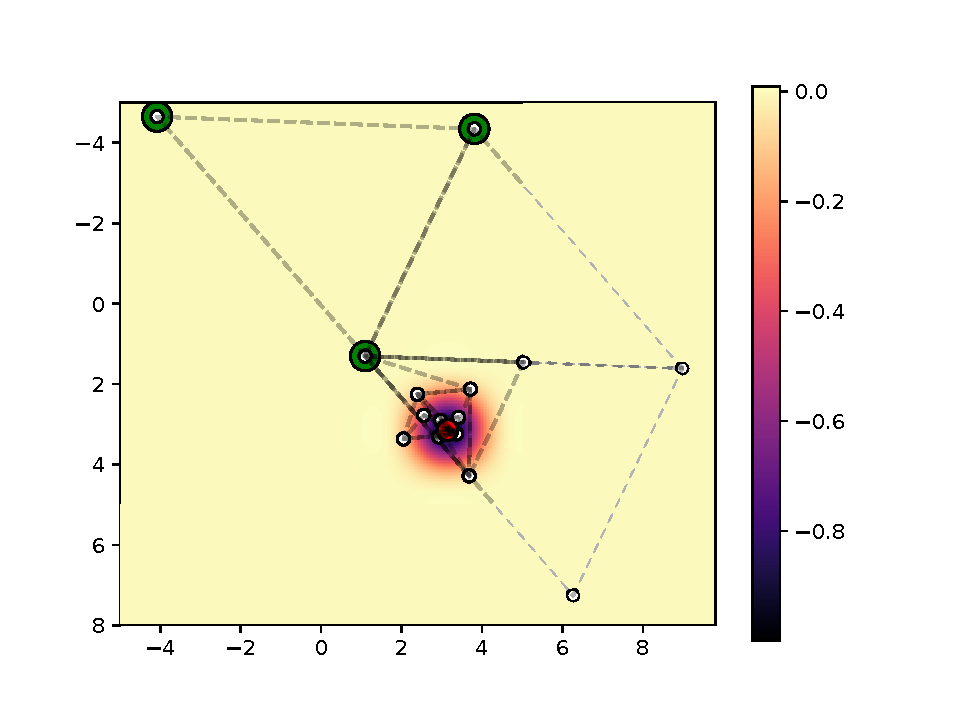
\includegraphics[width = .45\textwidth,trim={1cm 0 1cm 1.2cm}, clip]{Immagini/AbsoluteEasom1.pdf}} 
	\subfloat[]{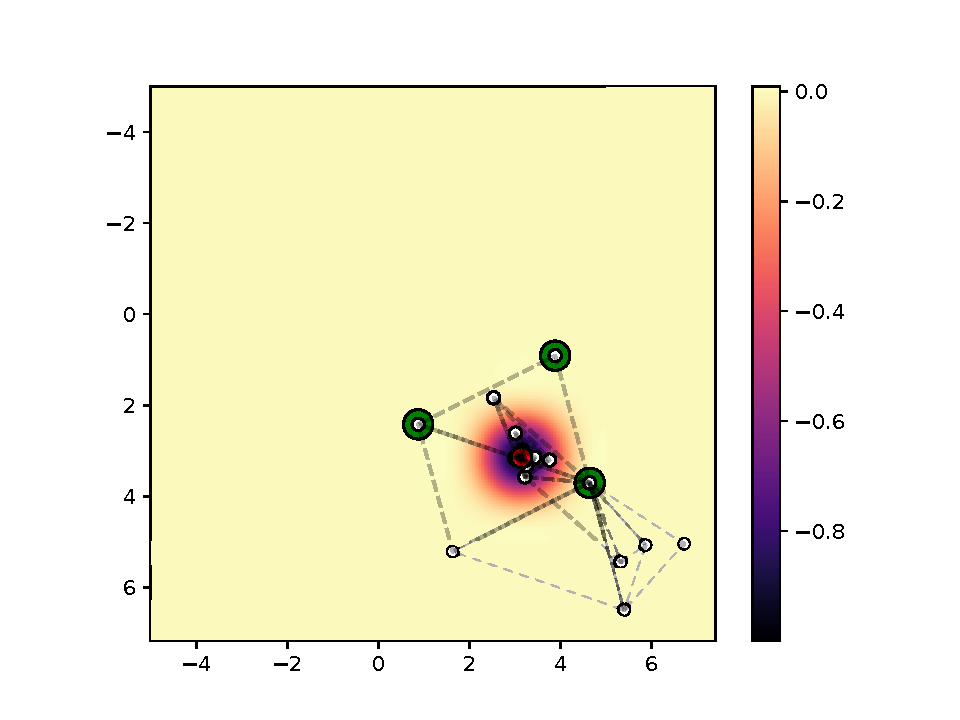
\includegraphics[width =  .45\textwidth,trim={1cm 0 1cm 1.2cm}, clip]{Immagini/AbsoluteEasom2.pdf}}\\
	\subfloat[]{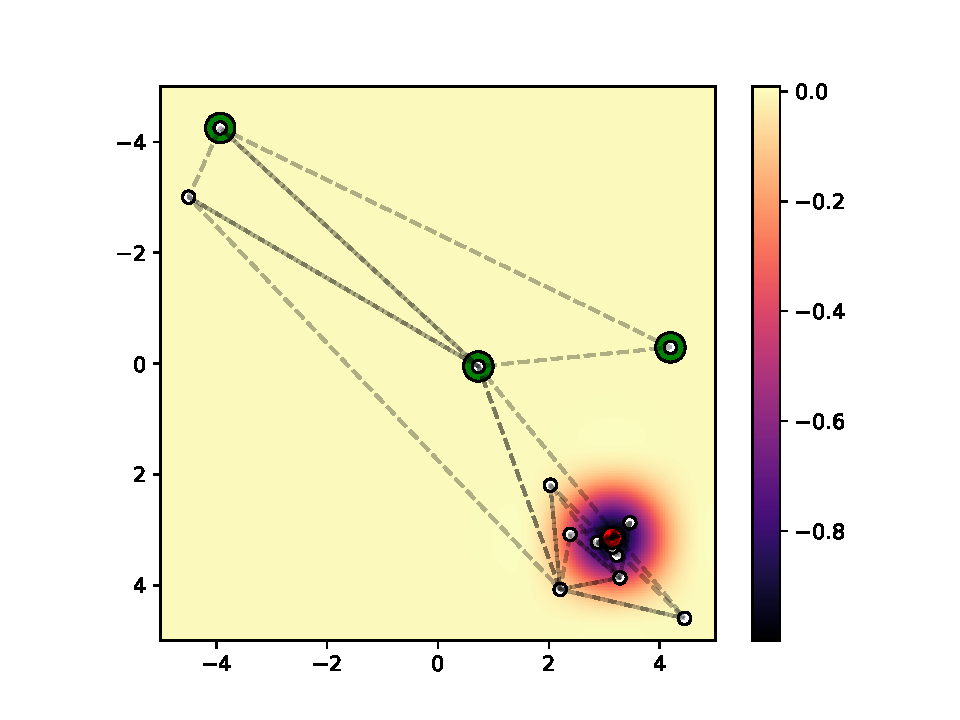
\includegraphics[width = .45\textwidth,trim={1cm 0 1cm 1cm}, clip]{Immagini/AbsoluteEasom3.pdf}}
	\subfloat[]{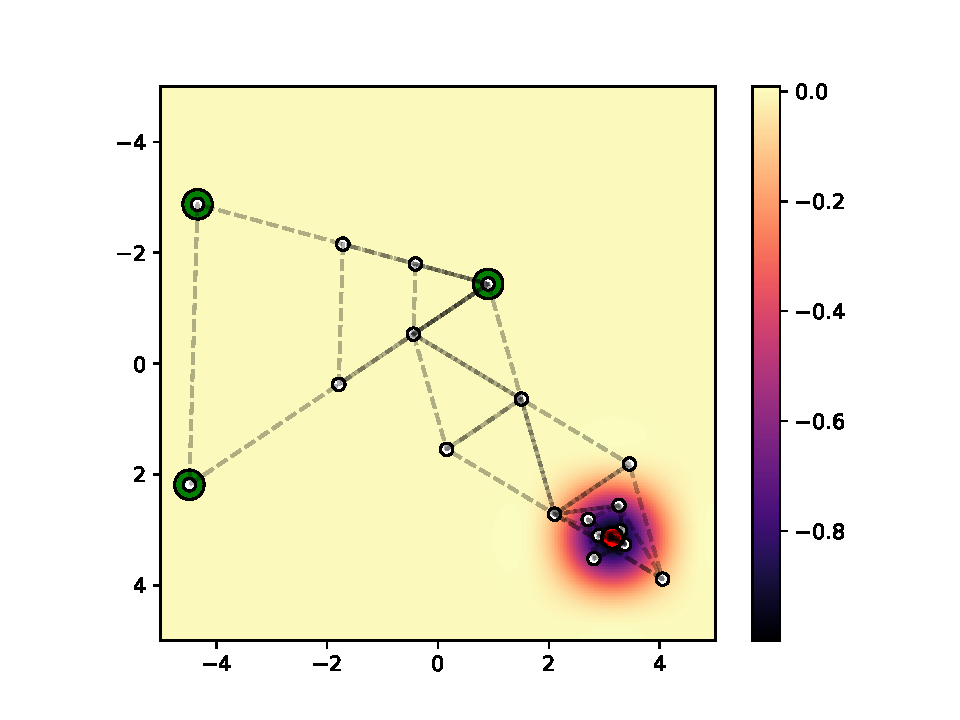
\includegraphics[width = .45\textwidth,trim={1cm 0 1cm 1cm}, clip]{Immagini/AbsoluteEasom4.pdf}} \\
	\subfloat[]{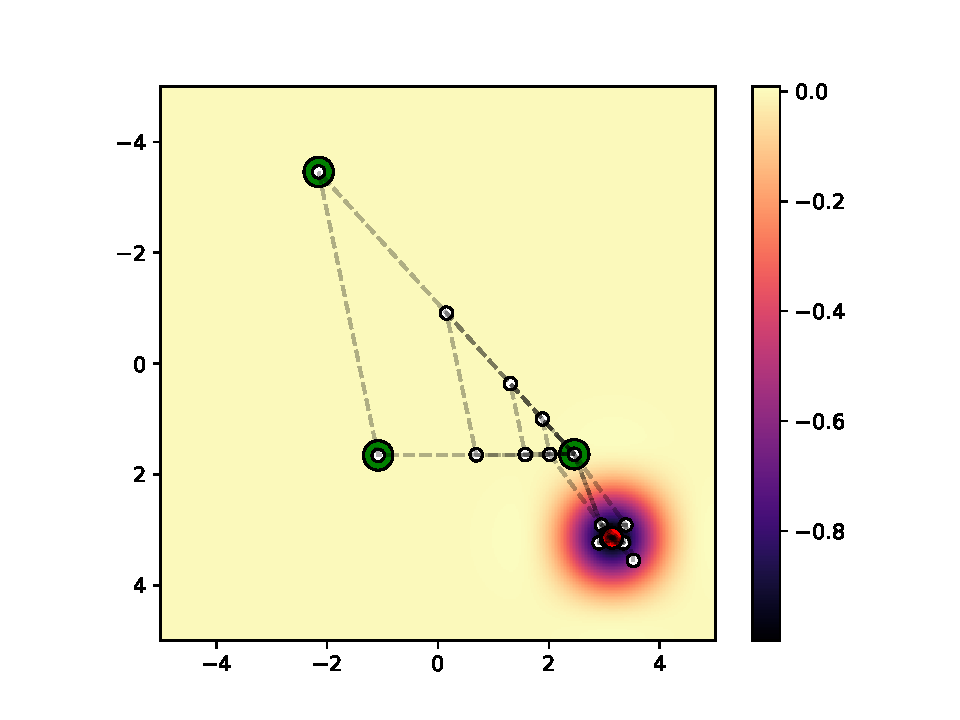
\includegraphics[width = .45\textwidth,trim={1cm 0 1cm 1cm}, clip]{Immagini/AbsoluteEasom5.pdf}}
	\subfloat[]{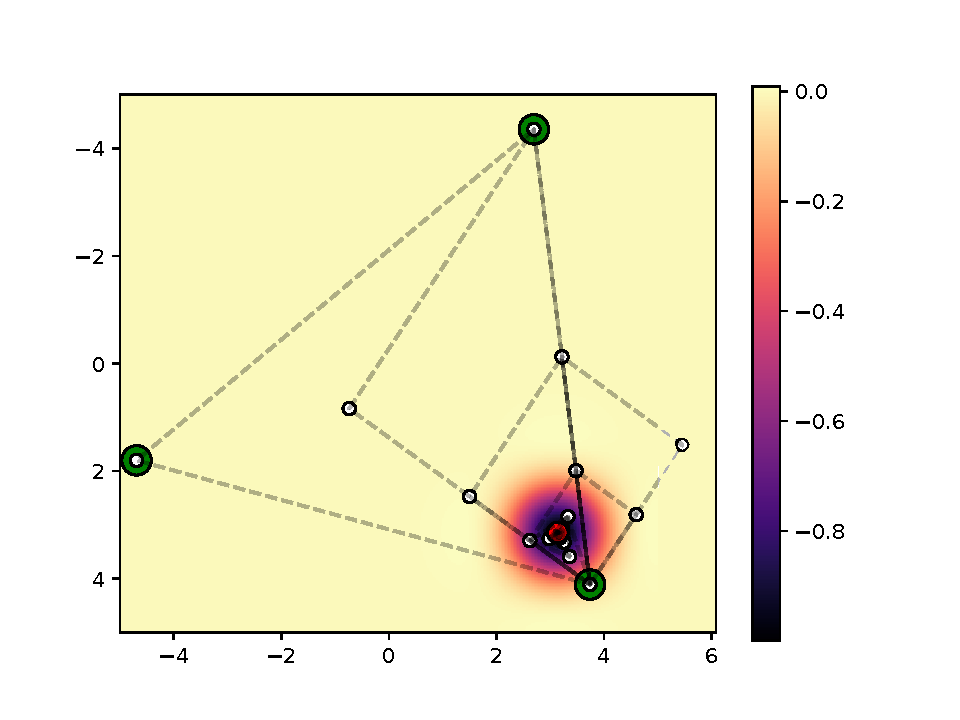
\includegraphics[width = .45\textwidth,trim={1cm 0 1cm 1cm}, clip]{Immagini/AbsoluteEasom6.pdf}}
	\label{fig:AbsoluteEasom}
\end{figure}

\begin{figure}
	\centering
	\caption{Sei istanze in cui il simplesso ha individuato dei minimi locali sul plateau della funzione di Easom.}
	
	\subfloat[]{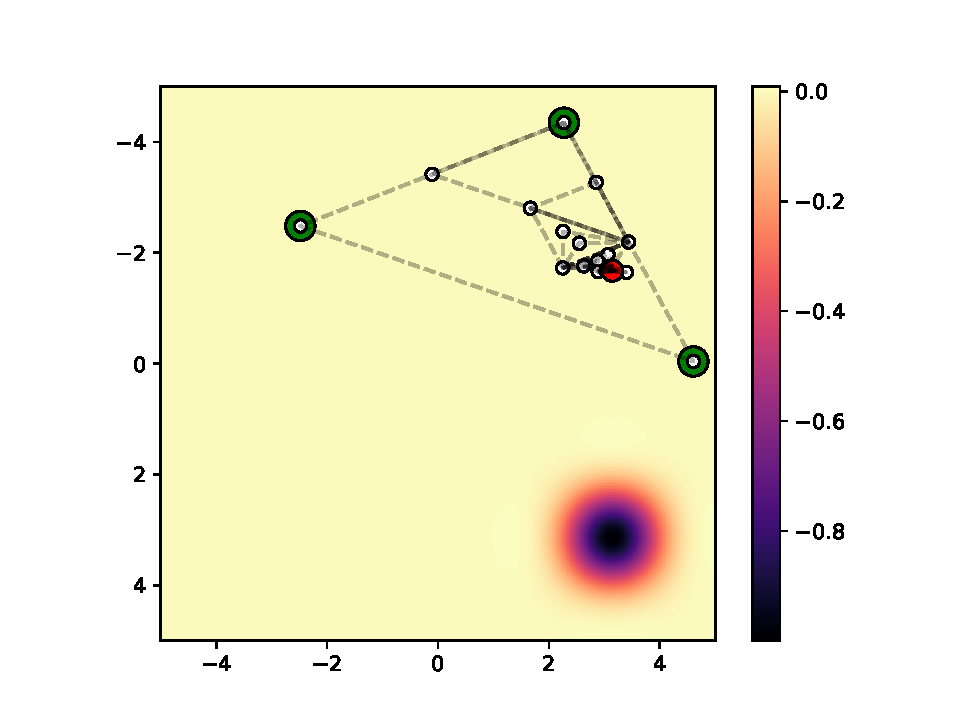
\includegraphics[width = .45\textwidth,trim={1cm 0 1cm 1cm}, clip]{Immagini/RelativeEasom1.pdf}} 
	\subfloat[]{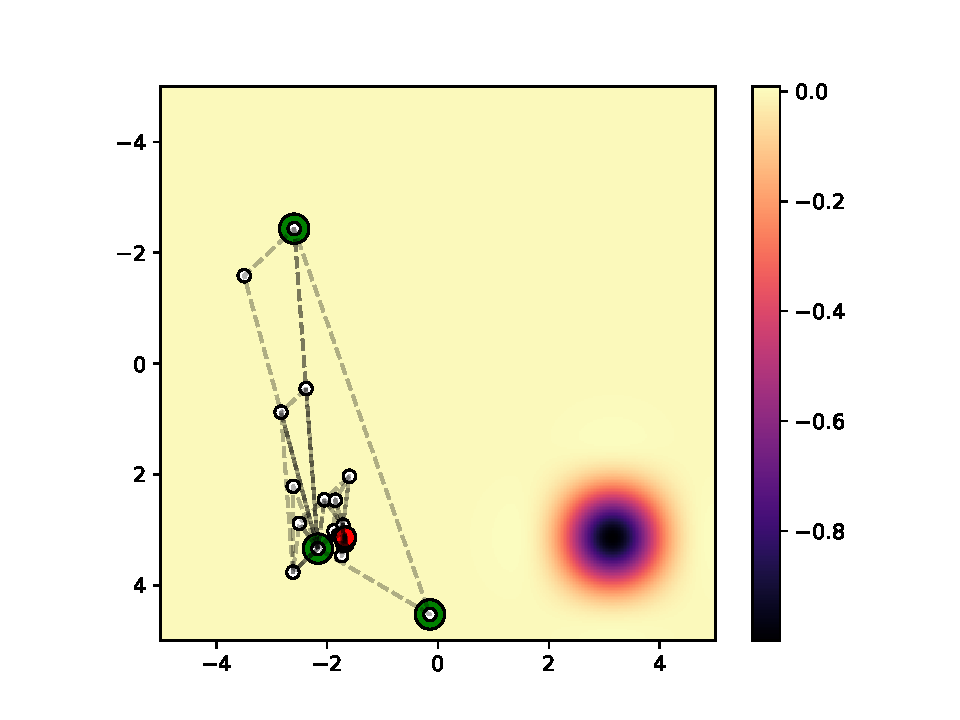
\includegraphics[width = .45\textwidth,trim={1cm 0 1cm 1cm}, clip]{Immagini/RelativeEasom2.pdf}}\\
	\subfloat[]{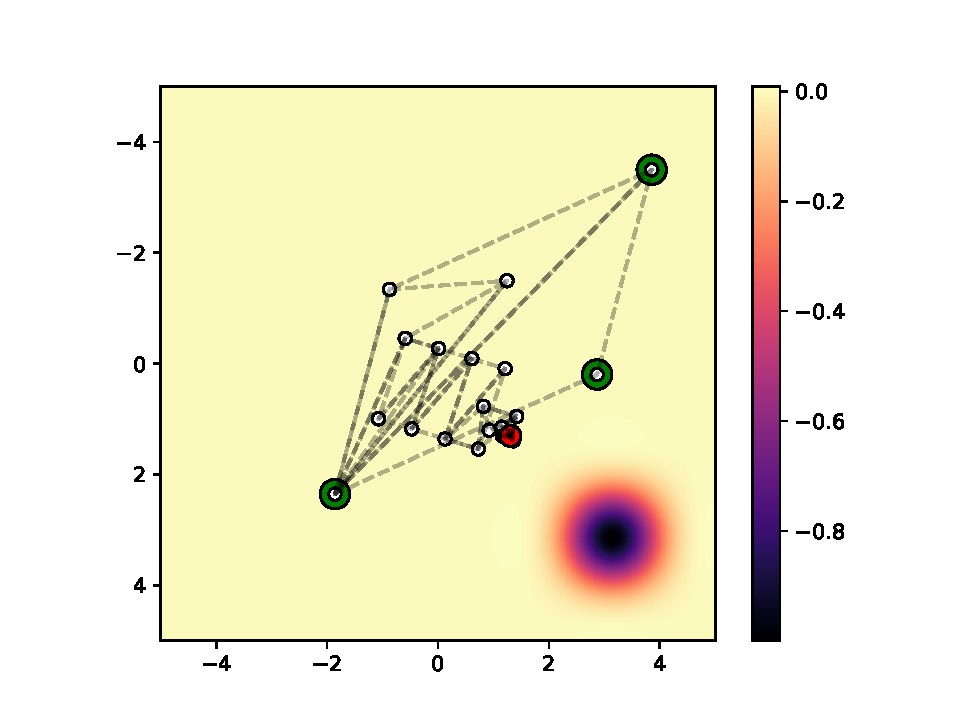
\includegraphics[width = .45\textwidth,trim={1cm 0 1cm 1cm}, clip]{Immagini/RelativeEasom3.pdf}}
	\subfloat[]{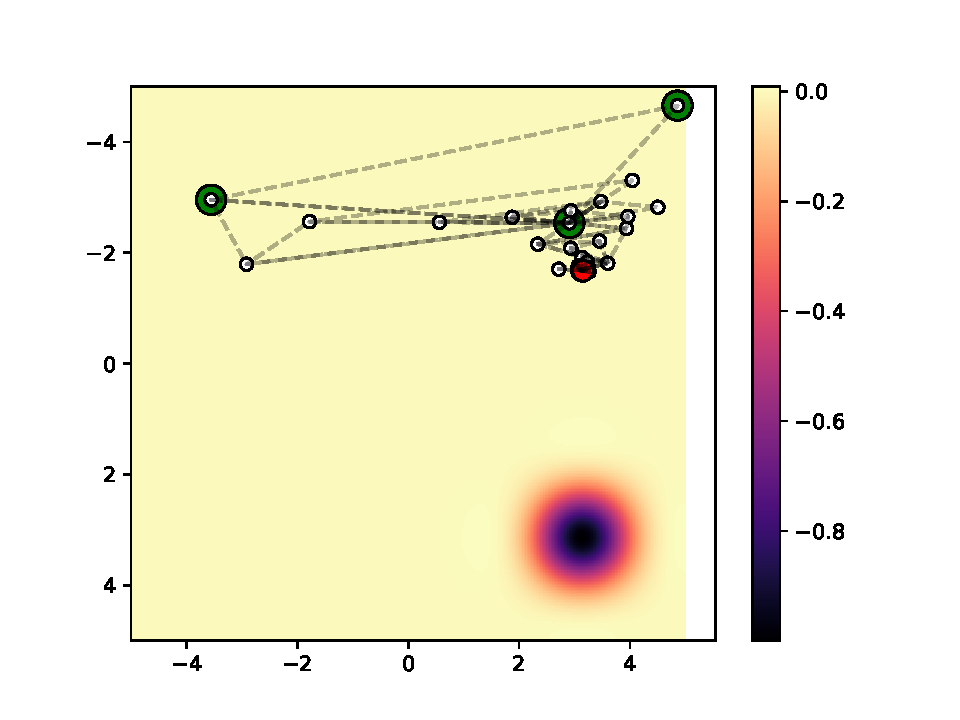
\includegraphics[width = .45\textwidth,trim={1cm 0 1cm 1cm}, clip]{Immagini/RelativeEasom4.pdf}} \\
	\subfloat[]{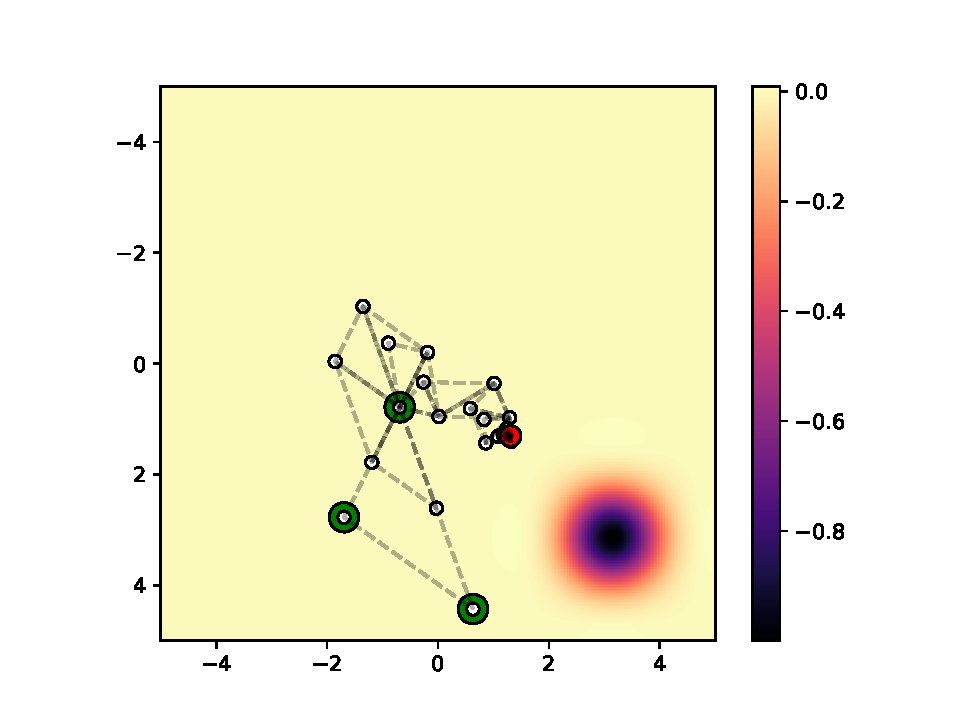
\includegraphics[width = .45\textwidth,trim={1cm 0 1cm 1cm}, clip]{Immagini/RelativeEasom5.pdf}}
	\subfloat[]{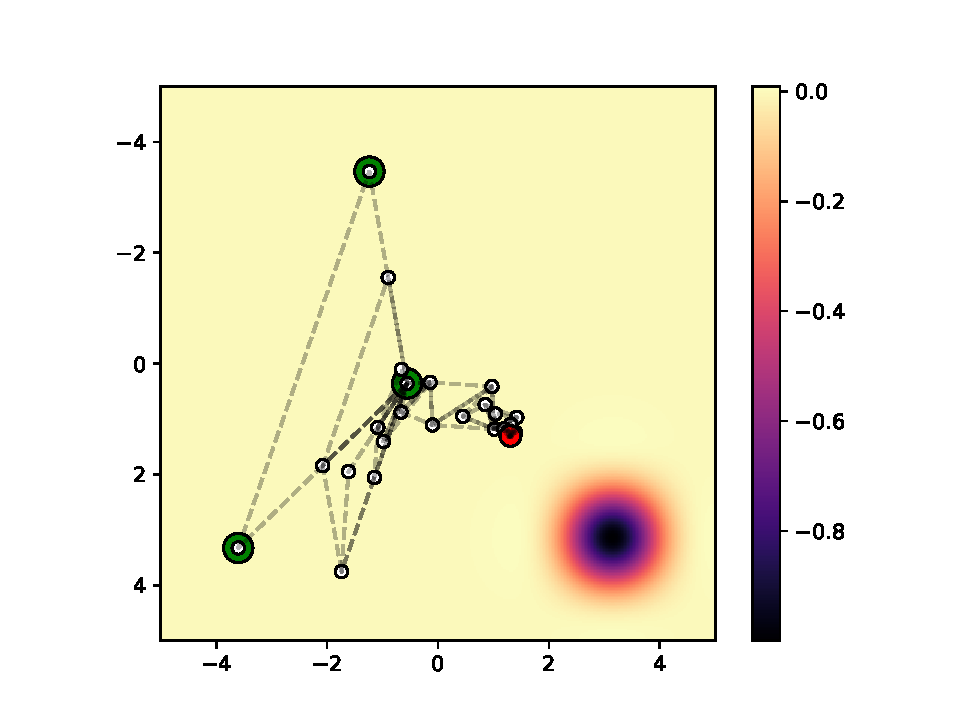
\includegraphics[width = .45\textwidth,trim={1cm 0 1cm 1cm}, clip]{Immagini/RelativeEasom6.pdf}}
	\label{fig:RelativeEasom}
\end{figure}

\newpage

\subsection*{Funzione di Goldstein-Price}

Anche in questo caso le coordinate iniziali dei vertici sono state generate casualmente nell'intervallo uniforme $\![-5,5]$. Il minimo locale globale è noto essere $f(3,4) = 1$, ragion per cui tale area di ricerca ci è sembrata senz'altro adeguata.\\

\noindent I grafici in \figurename~\ref{fig:Goldstein} evidenziano chiaramente una \emph{vallata circolare} puntualmente selezionata dall'evoluzione del simplesso. Su di essa effettivamente risiede il minimo globale: si tratta di una circonferenza centrata in $(0,0)$ e con raggio $R=5$. In particolare tutte le istanze della routine hanno trovato convergenza in due minimi: quello globale e uno locale nei dintorni di $(5,0)$.\\

\noindent Tali risultati appaiono del tutto ragionevoli se confrontati con il grafico in scala logaritmica riportato in \figurename~\ref{fig:GoldsteinLog}, che evidenzia appunto la struttura della corona circolare individuata dall'evoluzione del simplesso: si tratta di un vallata ad anello con fondo sostanzialmente piatto, tranne che per una "cresta" di minimi locali posizionati circa nel primo quadrante; i due più profondi sembrano essere proprio quelli selezionati dalla nostra routine.

\vfill

\begin{figure}[h!]
	\centering
	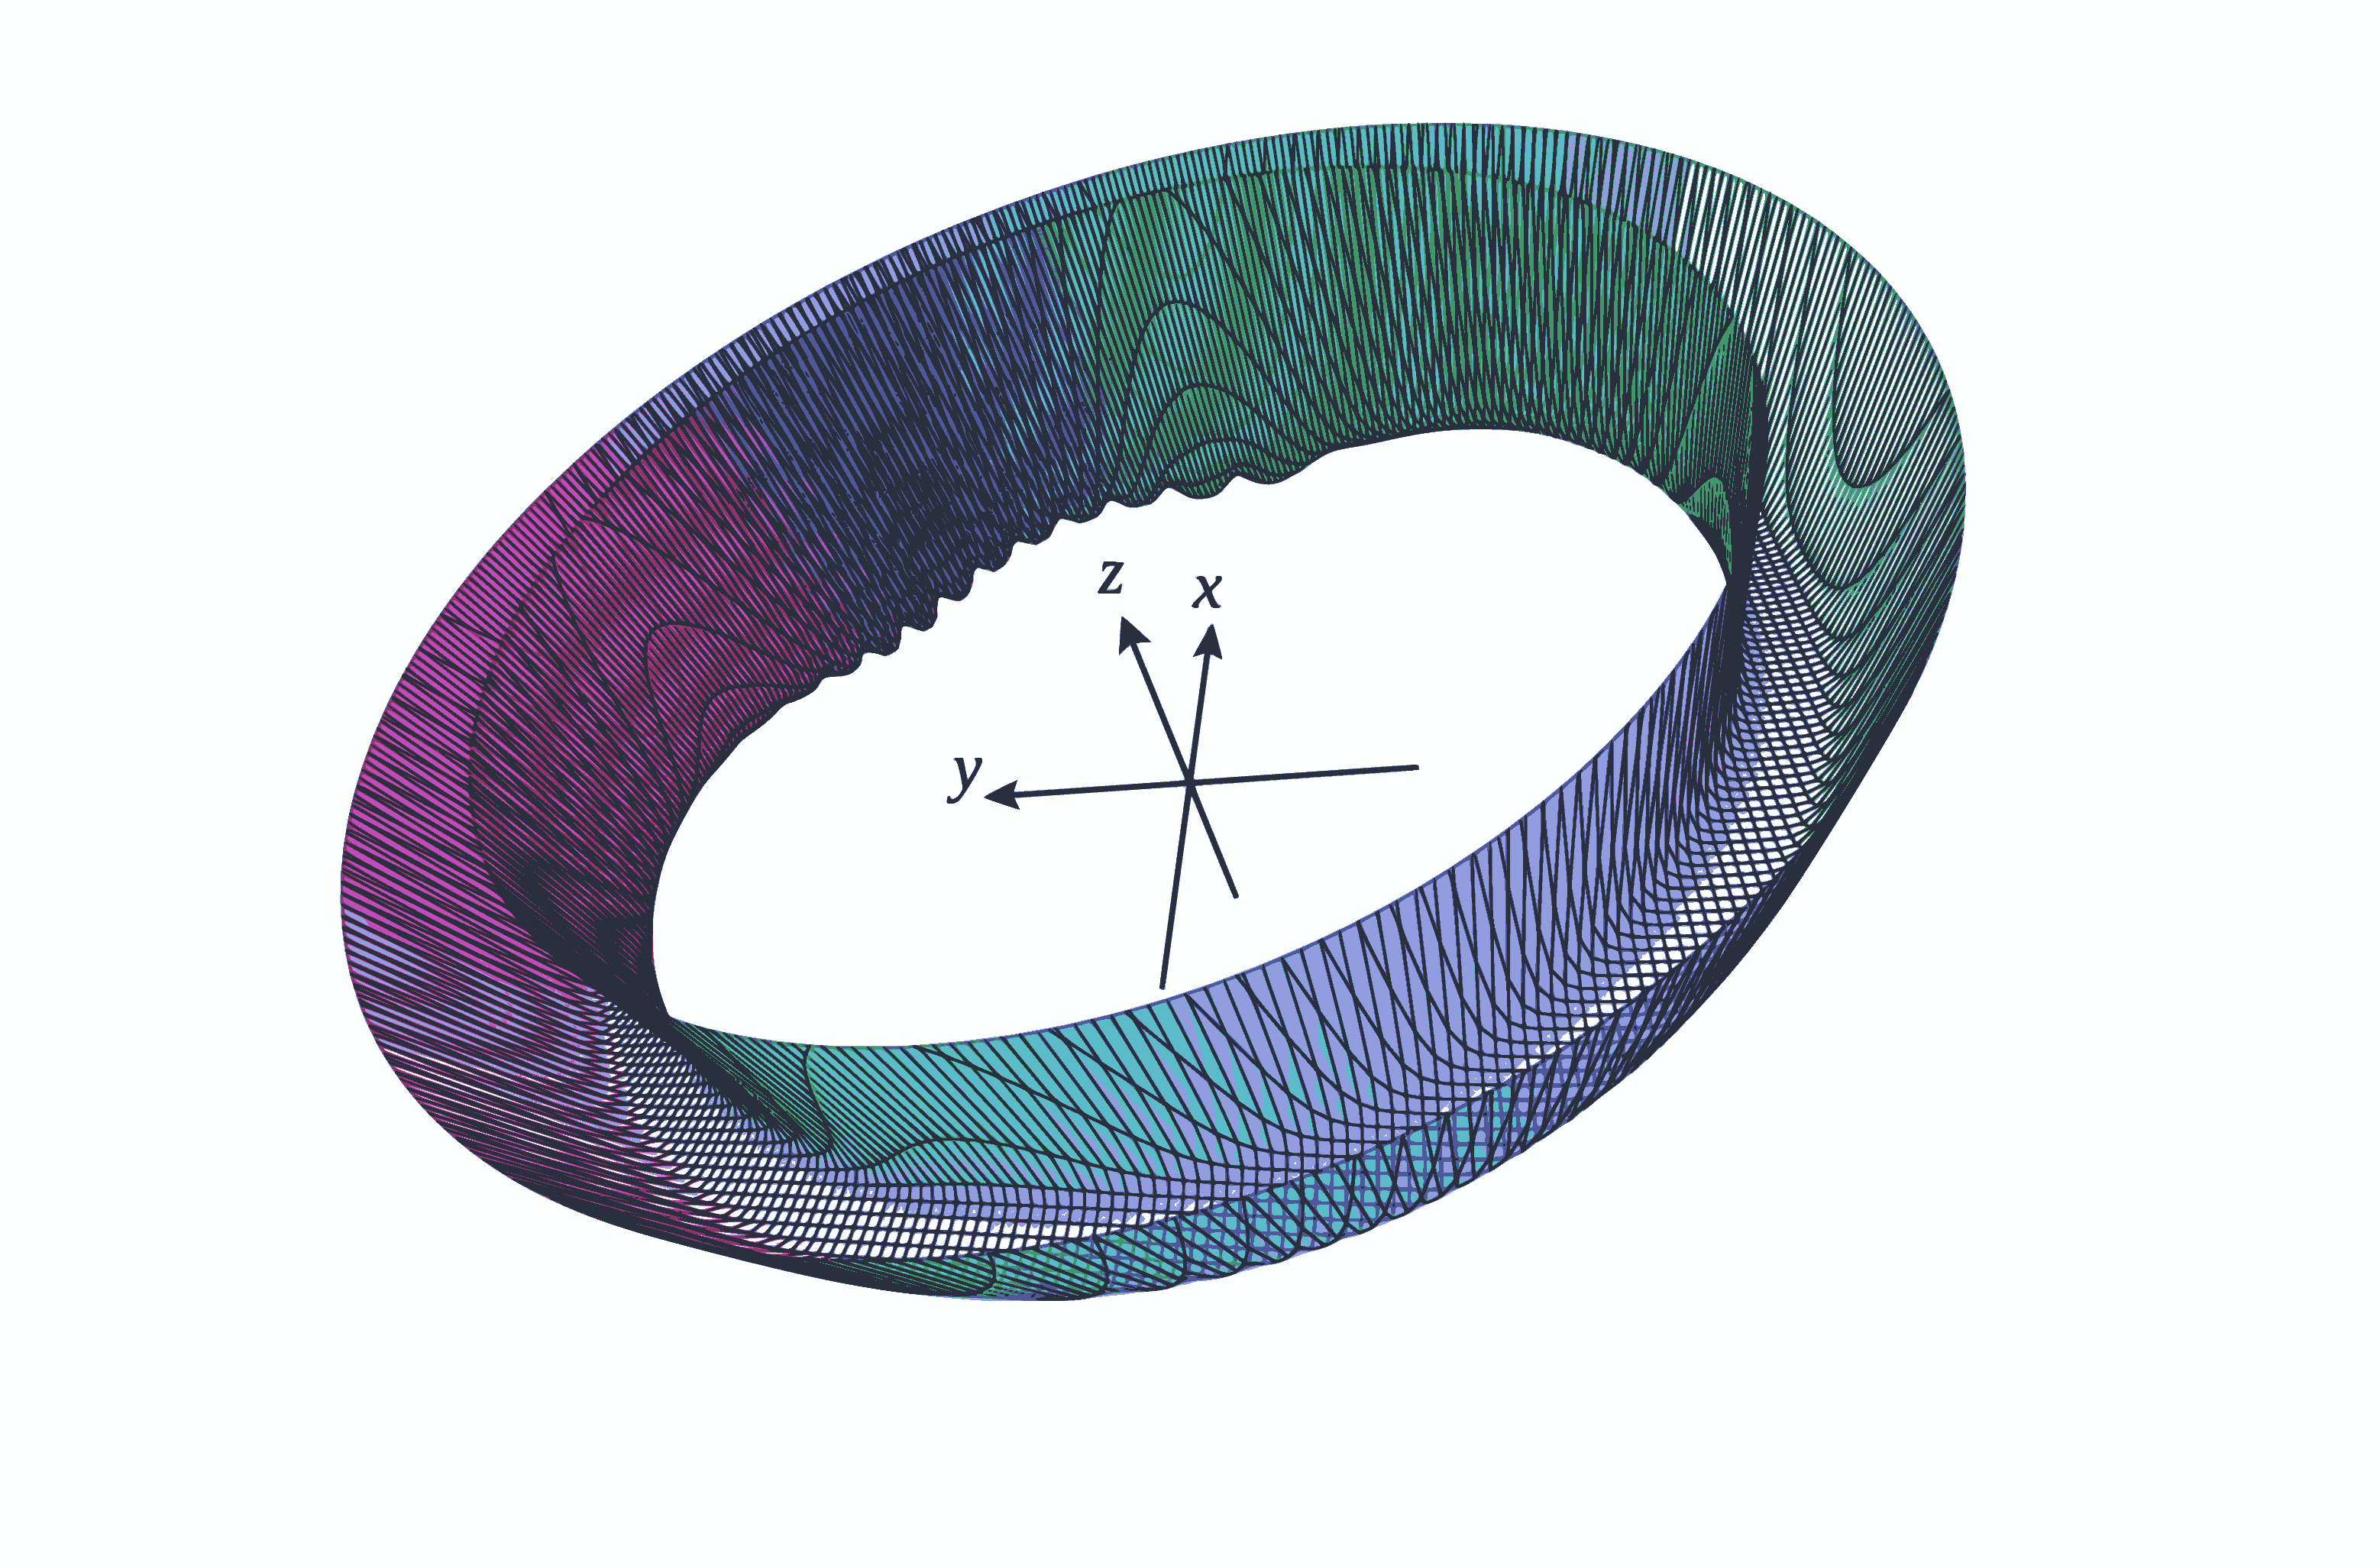
\includegraphics[width=1\linewidth, trim={5cm 5cm 5cm 1cm}, clip]{Immagini/GoldsteinLog.pdf}
	\caption{Grafico logaritmico della \emph{vallata circolare} in cui si trova il minimo globale della funzione di Goldstein-Price.}
	\label{fig:GoldsteinLog}
\end{figure}

\vfill

\begin{figure} 
	\centering
	\caption{Sei istanze che evidenziano la \emph{vallata circolare} della funzione di Goldstein-Price. In particolare (a), (c) e~(f) hanno selezionato il minimo globale $f(3,4) = 1$. La {colormap} è in scala logaritmica.}
	
	\subfloat[]{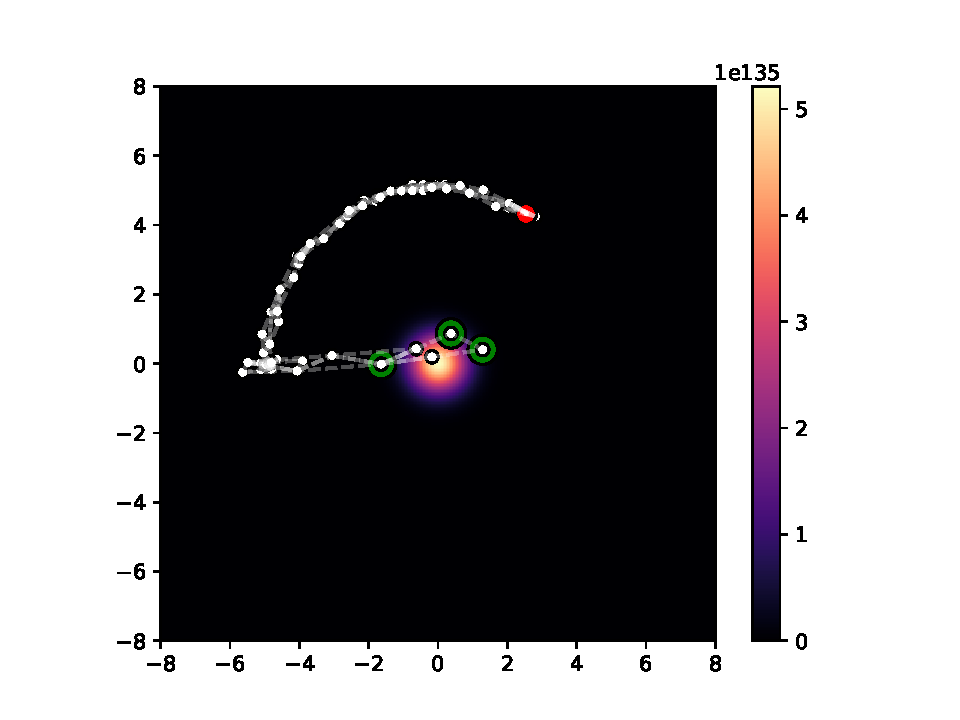
\includegraphics[width = .45\textwidth,trim={1cm 0 1cm 1cm}, clip]{Immagini/Goldstein1.pdf}} 
	\subfloat[]{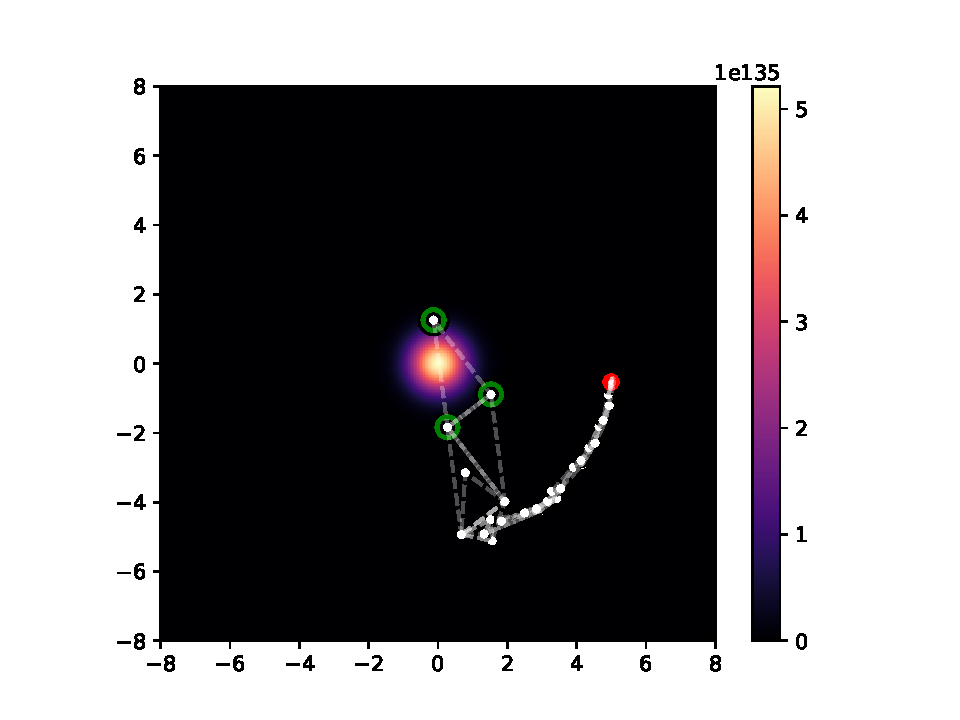
\includegraphics[width = .45\textwidth,trim={1cm 0 1cm 1cm}, clip]{Immagini/Goldstein2.pdf}}\\
	\subfloat[]{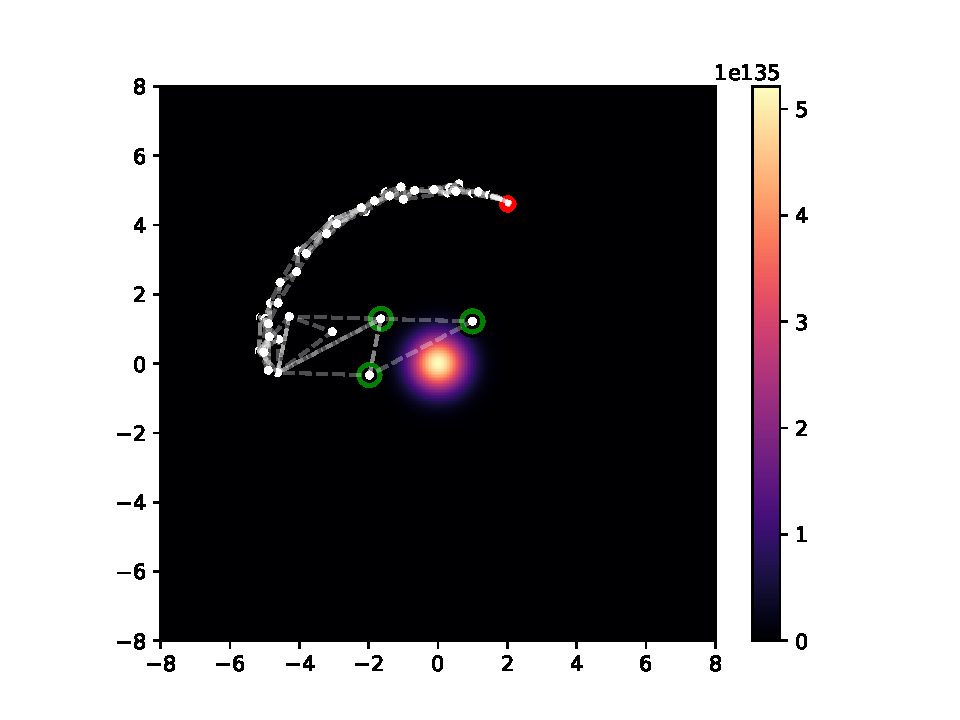
\includegraphics[width = .45\textwidth,trim={1cm 0 1cm 1cm}, clip]{Immagini/Goldstein3.pdf}}
	\subfloat[]{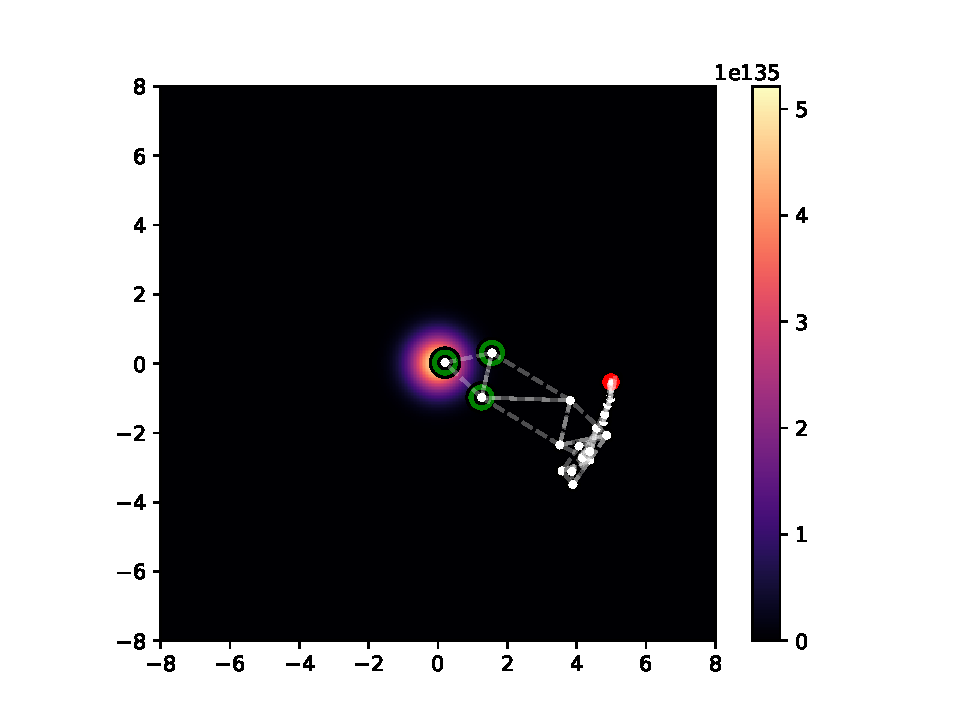
\includegraphics[width = .45\textwidth,trim={1cm 0 1cm 1cm}, clip]{Immagini/Goldstein4.pdf}} \\
	\subfloat[]{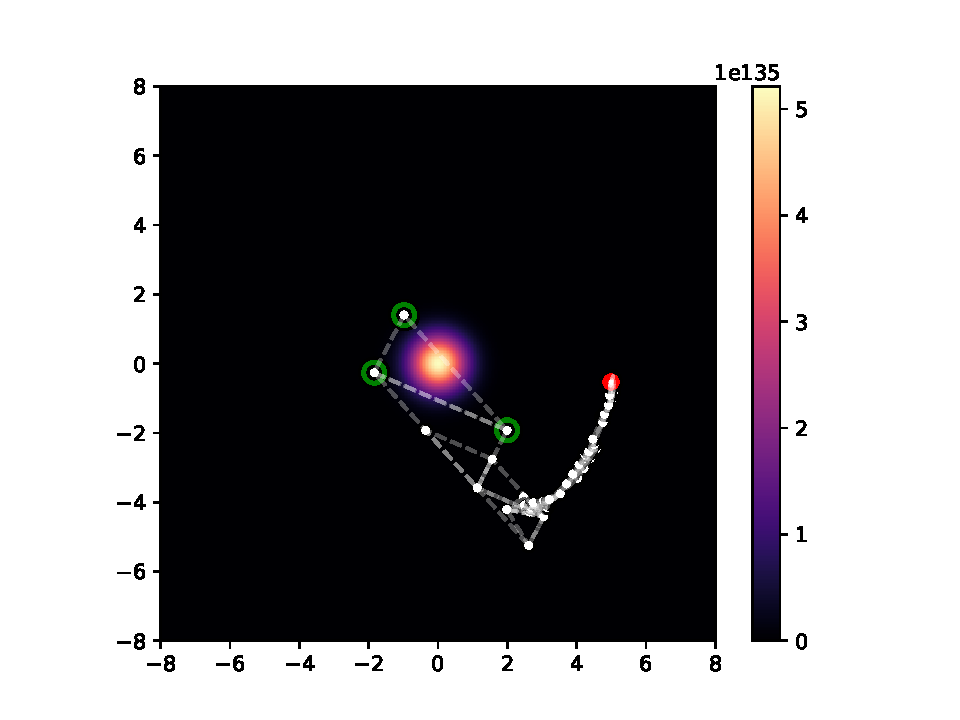
\includegraphics[width = .45\textwidth,trim={1cm 0 1cm 1cm}, clip]{Immagini/Goldstein5.pdf}}
	\subfloat[]{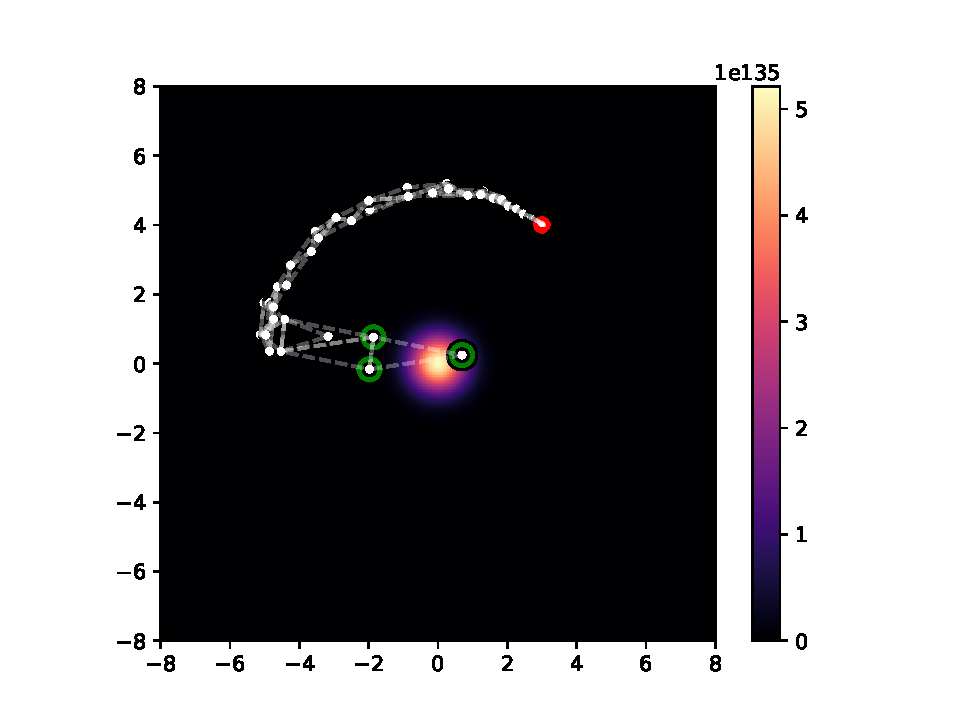
\includegraphics[width = .45\textwidth,trim={1cm 0 1cm 1cm}, clip]{Immagini/Goldstein6.pdf}}
	\label{fig:Goldstein}
\end{figure}

\newpage

\subsection*{Funzione di Bukin Nr.~6}

In \figurename~\ref{fig:EasomPlot} è riportato il grafico della funzione Nr.6 di Bukin. \`E evidente la presenza di una "cresta" di minimi locali posizionati lungo una fascia che interseca perpendicolarmente l'asse $\vec{x}$  nell'origine.\\

\noindent Estraendo coordinate uniformi  nella regione asimmetrica $x\in[-5,5]$, $y\in[-12,12]$ ne abbiamo individuati vari (Cfr. \figurename~\ref{fig:RelativeBukin}), anche relativamente lontani dal centro della fascia. Ne dedurremmo che i bordi della "cresta" non siano monotoni, anche se rimane il dubbio che in questo caso l'algoritmo implementato soffra di qualche criticità: il simplesso è sempre arrivato a convergere su intorni dati da una tolleranza di $\varepsilon=10^{-5}$ e valori inferiori hanno sempre prodotto tempi di calcolo eccessivamente prolungati.\\

\noindent Per quanto riguarda il minimo globale della funzione, posizionato lontano dalla cresta, in $\mathbf{x}_0 = (-10,1)$, abbiamo designato una regione stretta e mirata per la generazione dei vertici iniziali del simplesso - doppio intervallo uniforme $x\in[-12,-8]$, $y\in[0,3]$ - che ci ha permesso di arrivare ad approssimare con buona accuratezza il risultato:

\begin{align*}
\mathbf{x}_1 = (-9.94965119,  0.98995562) \enspace\enspace &\Longrightarrow \enspace\enspace f(\mathbf{x}_1) = 0.0005071942778401883\\
\mathbf{x}_2 = (-9.95151164,  0.99032607) \enspace\enspace &\Longrightarrow \enspace\enspace f(\mathbf{x}_2) = 0.0005075673516130408\\
\mathbf{x}_3 = (-9.95538255,  0.99109576) \enspace\enspace &\Longrightarrow \enspace\enspace f(\mathbf{x}_3) =0.0005122552638696298\\
\end{align*}

\noindent Il grafico dell'istanza che ha selezionato tali valori è riportato in \figurename~\ref{fig:AbsoluteBukin}.\\

\bigskip

\begin{figure}[h!]
	\centering
	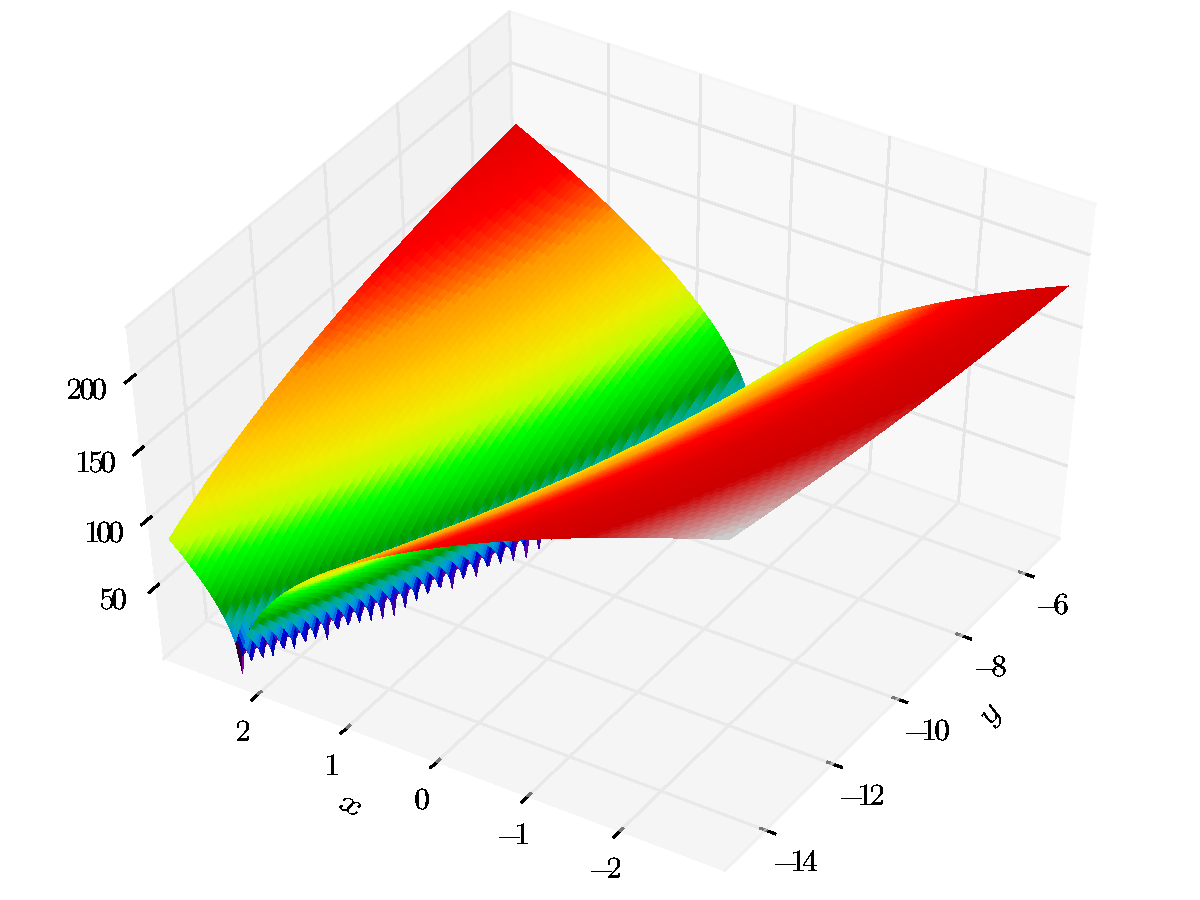
\includegraphics[width=0.85\linewidth]{Immagini/Bukin_function_6.pdf}
	\caption{Grafico 3D della funzione di Bukin Nr.~6. Da \texttt{Wikipedia} (Cfr. la nota a pié di pagina~\pageref{WikipediaFootnote}).}
	\label{fig:BukinPlot}
\end{figure}

\begin{figure}
	\centering
	\caption{Sei istanze mirate alla ricerca dei minimi locali sulla "cresta" della funzione Nr.6 di Bukin.}
	\subfloat[]{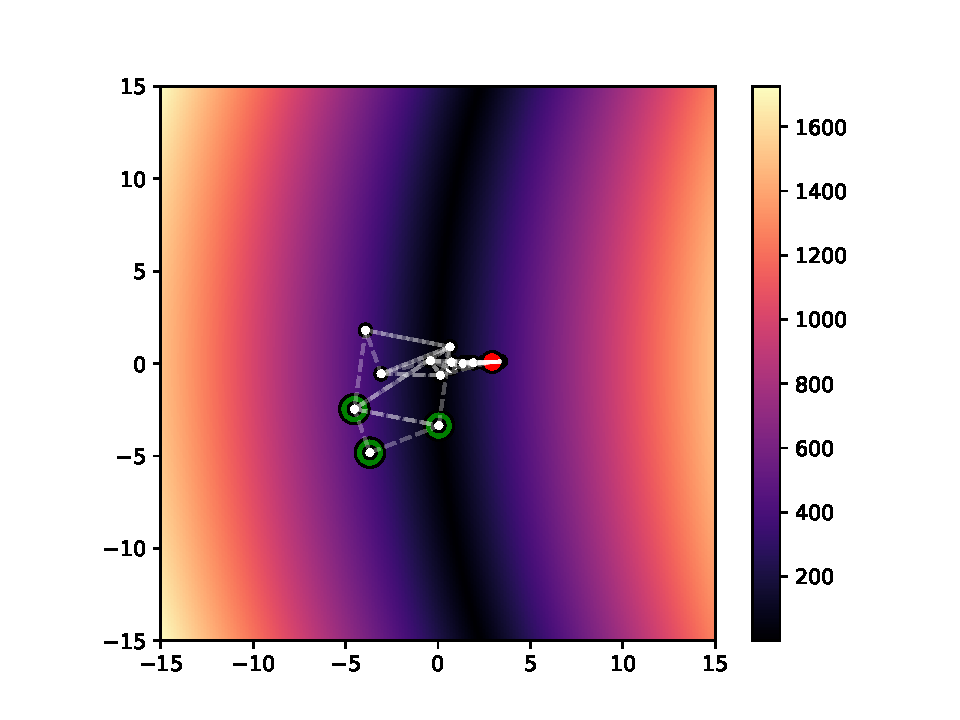
\includegraphics[width = .45\textwidth,trim={1cm 0 1cm 1cm}, clip]{Immagini/RelativeBukin1.pdf}} 
	\subfloat[]{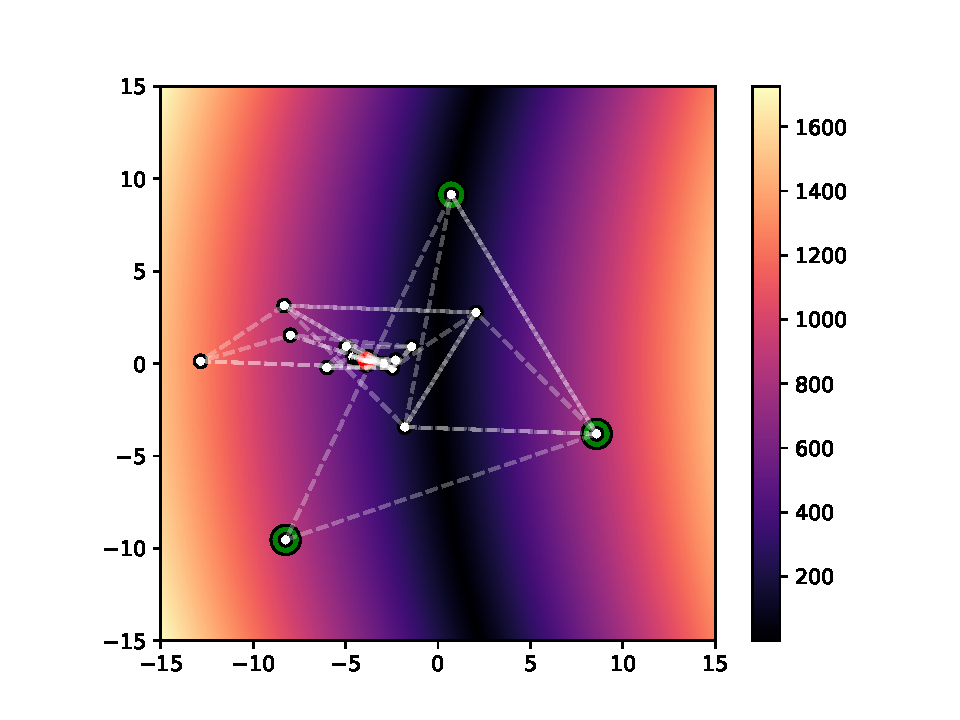
\includegraphics[width = .45\textwidth,trim={1cm 0 1cm 1cm}, clip]{Immagini/RelativeBukin2.pdf}}\\
	\subfloat[]{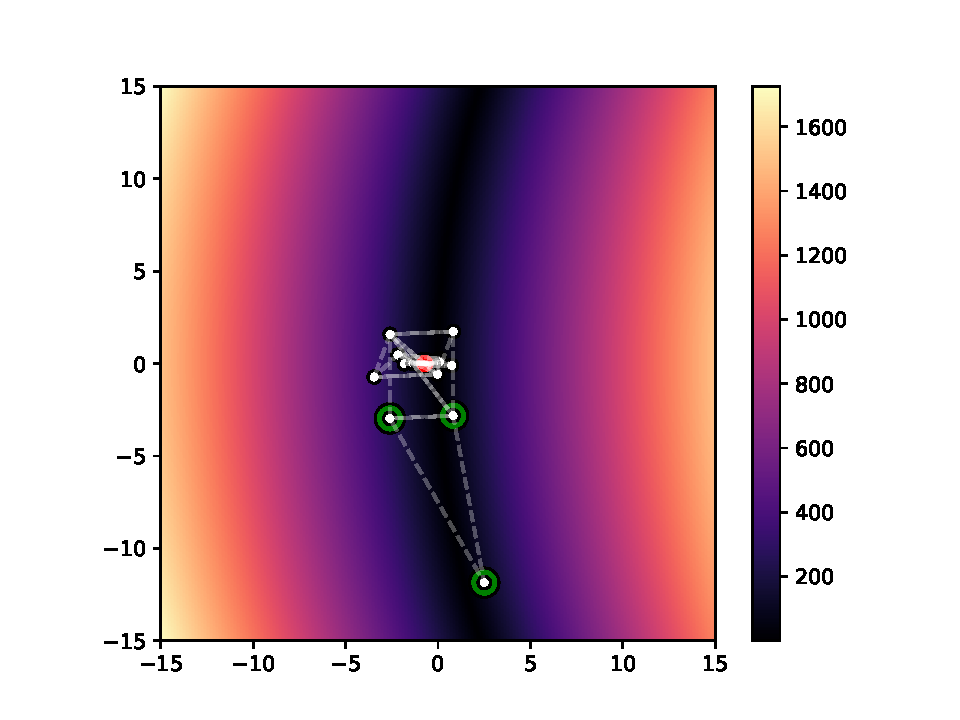
\includegraphics[width = .45\textwidth,trim={1cm 0 1cm 1cm}, clip]{Immagini/RelativeBukin3.pdf}}
	\subfloat[]{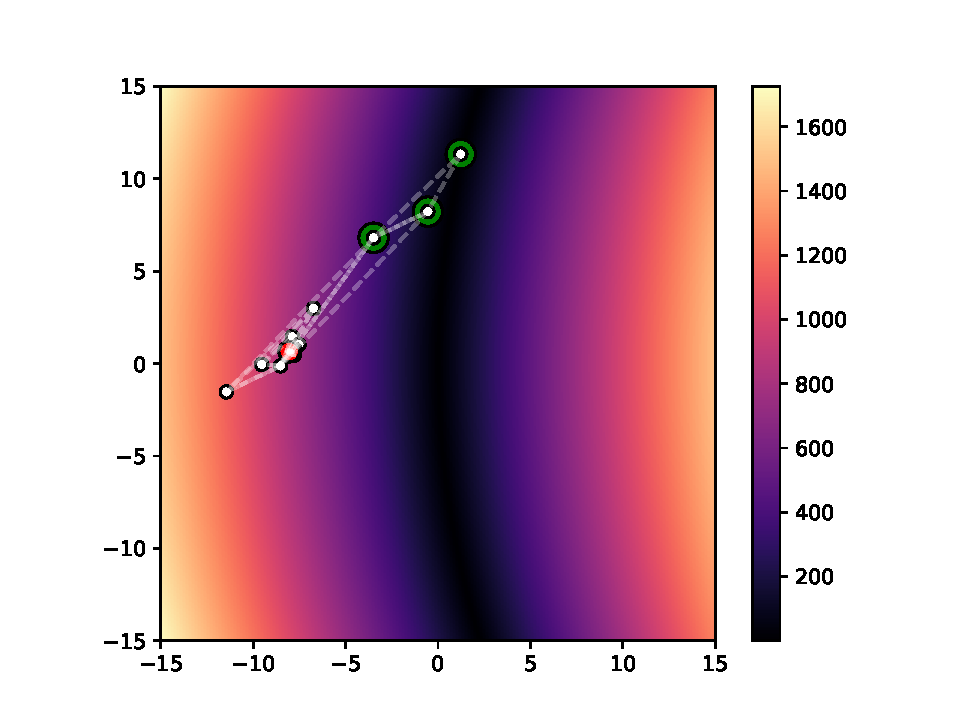
\includegraphics[width = .45\textwidth,trim={1cm 0 1cm 1cm}, clip]{Immagini/RelativeBukin4.pdf}} \\
	\subfloat[]{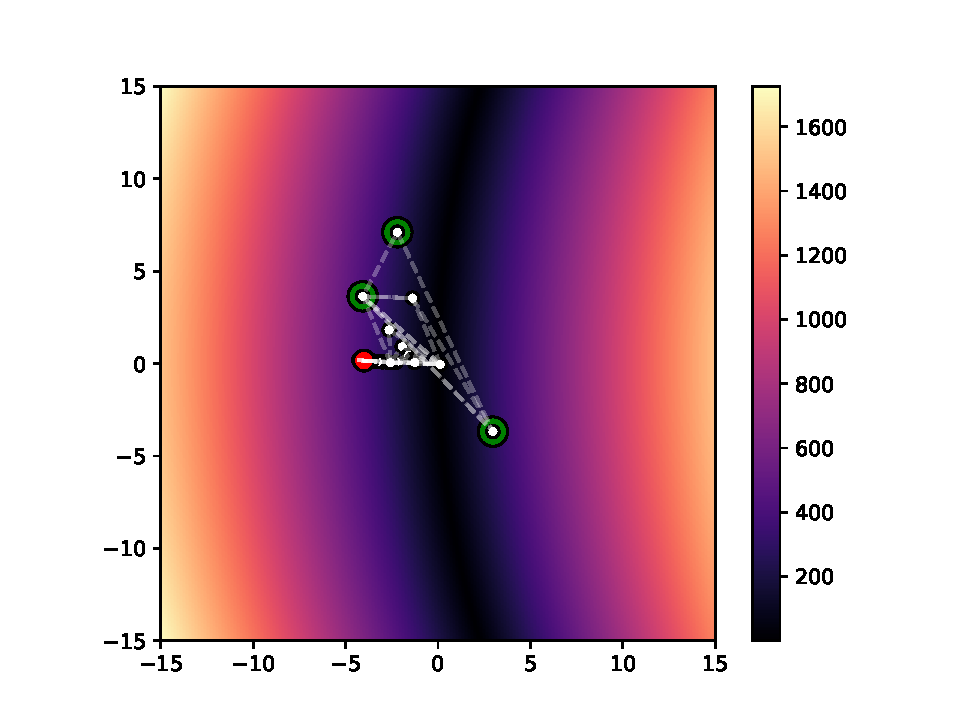
\includegraphics[width = .45\textwidth,trim={1cm 0 1cm 1cm}, clip]{Immagini/RelativeBukin5.pdf}}
	\subfloat[]{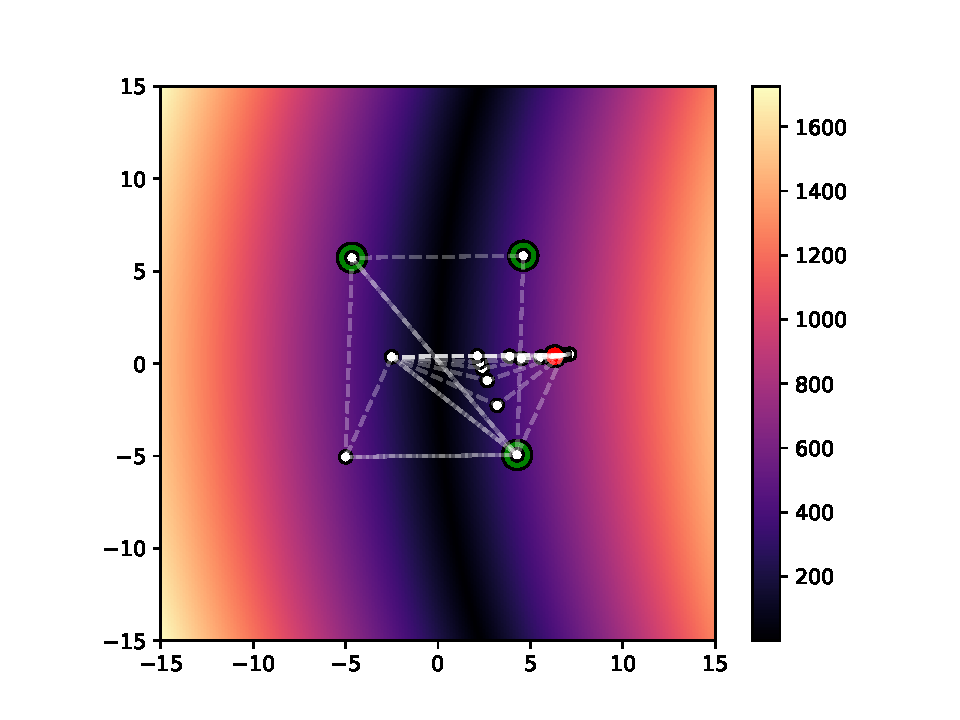
\includegraphics[width = .45\textwidth,trim={1cm 0 1cm 1cm}, clip]{Immagini/RelativeBukin6.pdf}}
	\label{fig:RelativeBukin}
\end{figure}

\begin{sidewaysfigure}
	\centering
	\caption{Ricerca del minimo globale della funzione Nr.~6 di Bukin.}
	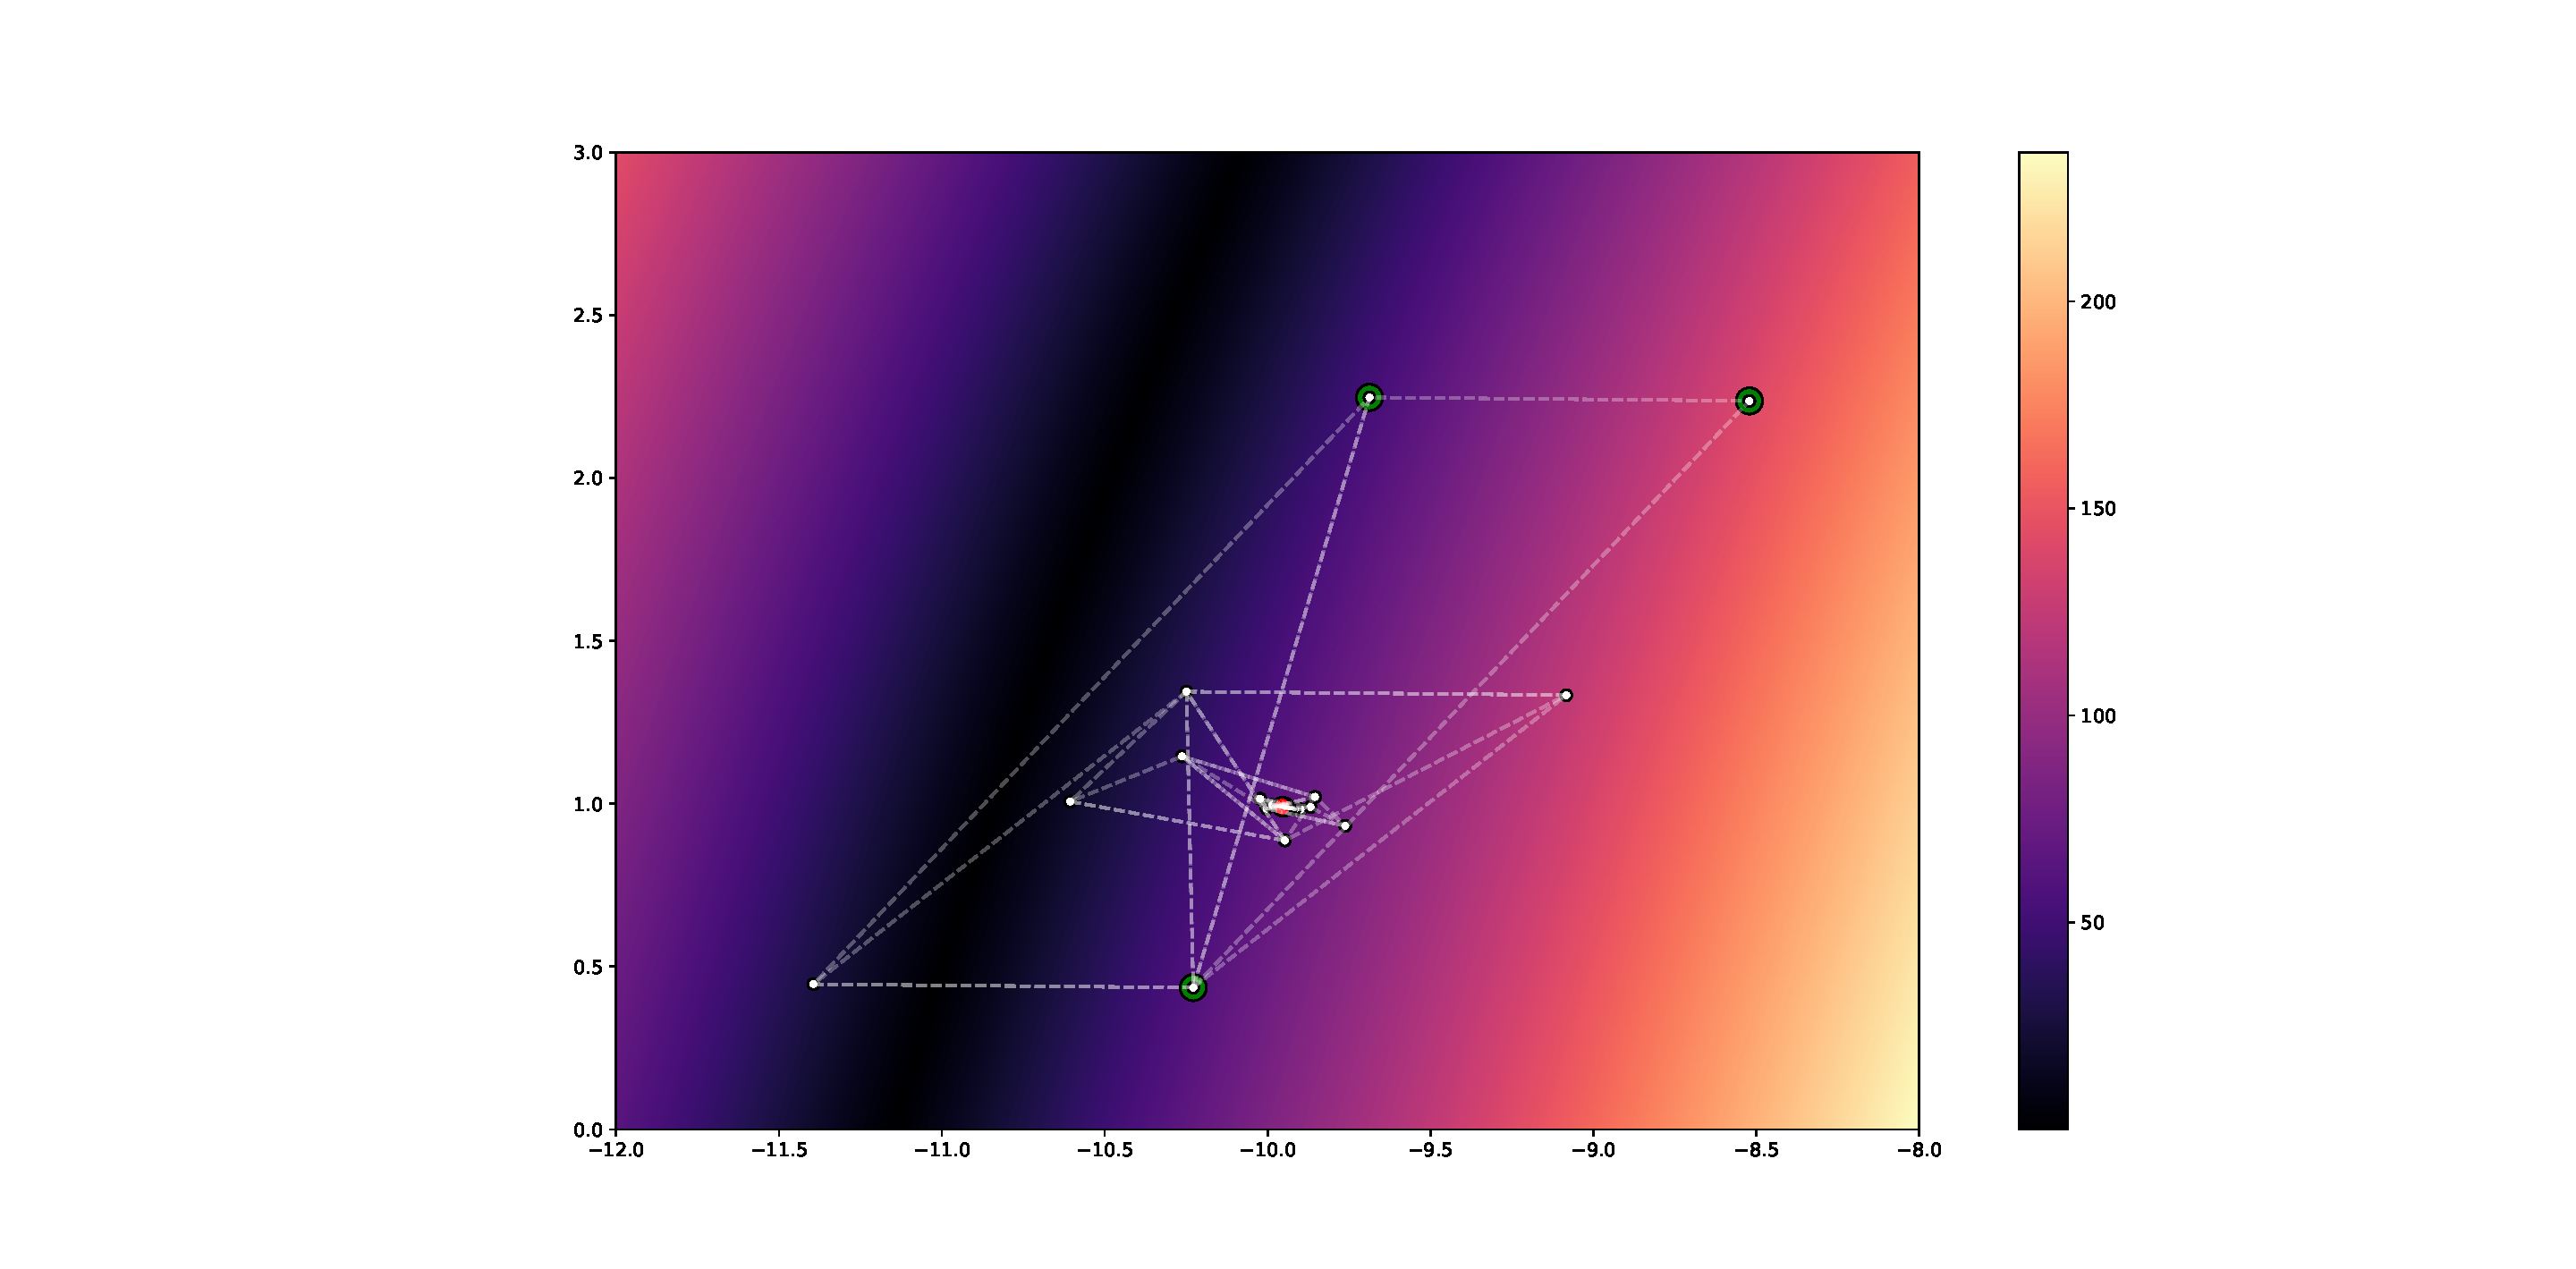
\includegraphics[width=\textwidth, trim={10cm 2cm 8cm 2cm}, clip]{Immagini/AbsoluteBukinBig.pdf}
	\label{fig:AbsoluteBukin}
\end{sidewaysfigure}

\newpage

\subsection*{Funzione di Booth}
\bigskip
La funzione di Booth è unimodale e convessa e in quanto tale presenta un unico minimo globale: $f(1,3) = 0$. Un~suo grafico è riportato in \figurename~\ref{fig:BoothPlot}.\\

\noindent In questa situazione l'algoritmo di Nelder-Mead è estremamente efficiente e si può generare il simplesso iniziale in una regione vasta a piacere. Noi abbiamo estratto le coordinate dei vertici nel doppio intervallo uniforme $[-15,15]$.\\

\noindent In \figurename~\ref{fig:Booth} sono riportati i grafici relativi a sei istanze della routine, ognuna delle quali ha dato convergenza al punto ottimo (entro $\varepsilon = 10^{-15}$ ) dopo qualche decina di passi.\\

\vfill

\begin{figure}[h!]
	\centering
	\includegraphics[width=\linewidth]{Immagini/Booth_function.pdf}
	\caption{Grafico 3D della funzione di Booth. Da \texttt{Wikipedia} (Cfr. la nota a pié di pagina~\pageref{WikipediaFootnote}).}
	\label{fig:BoothPlot}
\end{figure}

\vfill

\begin{figure}
	\centering
		\caption{Sei istanze in cui il simplesso è andato a convergere sul minimo globale della funzione di Booth.}
	\subfloat[]{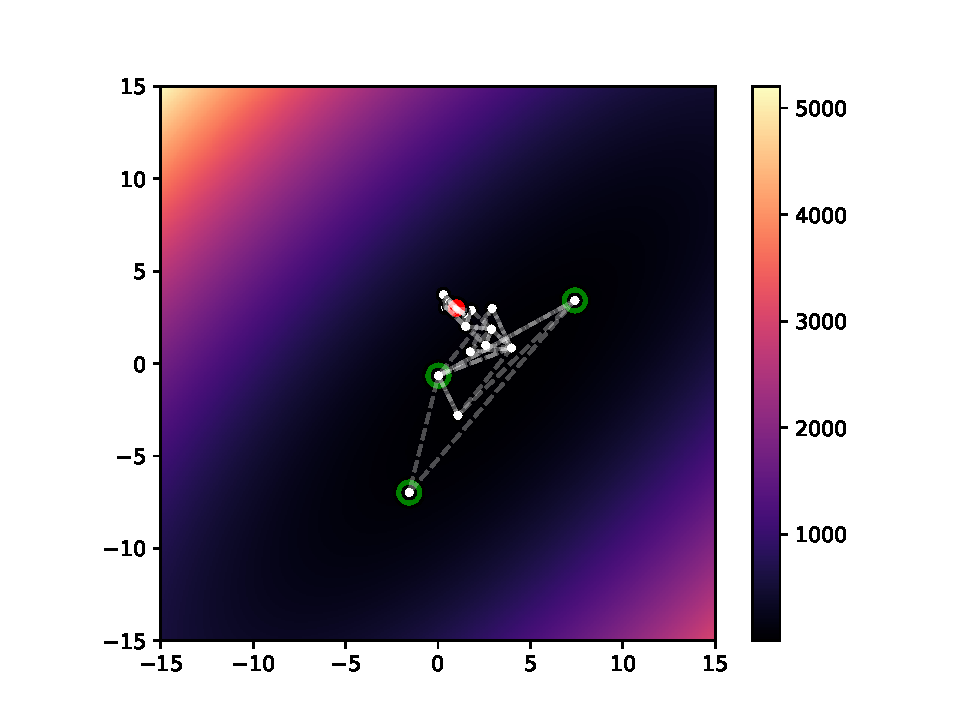
\includegraphics[width = .45\textwidth,trim={1cm 0 1cm 1cm}, clip]{Immagini/Booth1.pdf}} 
	\subfloat[]{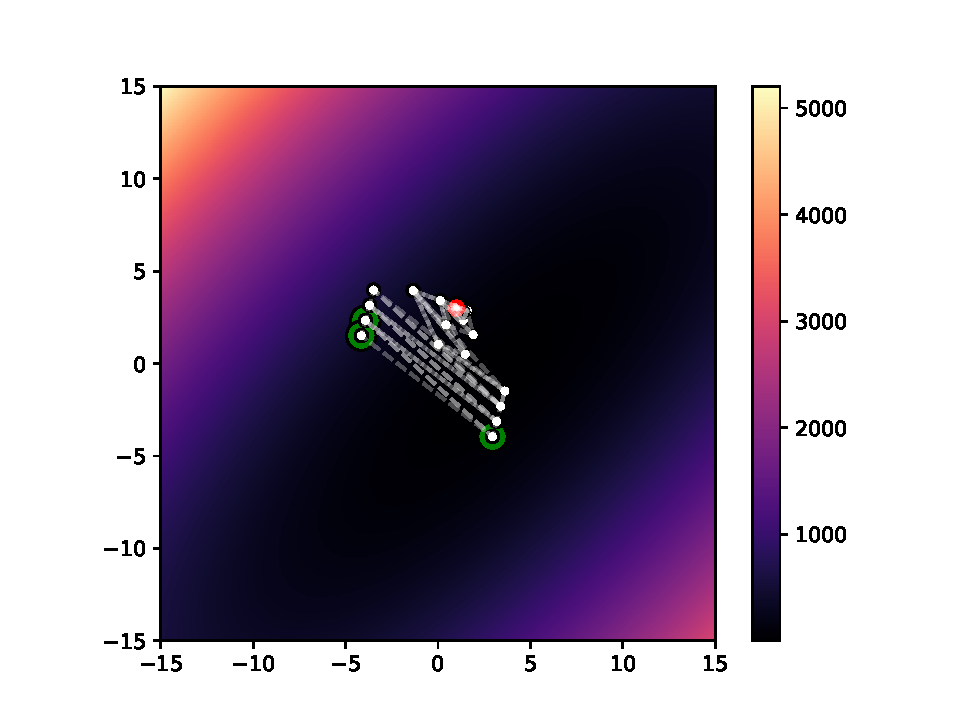
\includegraphics[width = .45\textwidth,trim={1cm 0 1cm 1cm}, clip]{Immagini/Booth2.pdf}}\\
	\subfloat[]{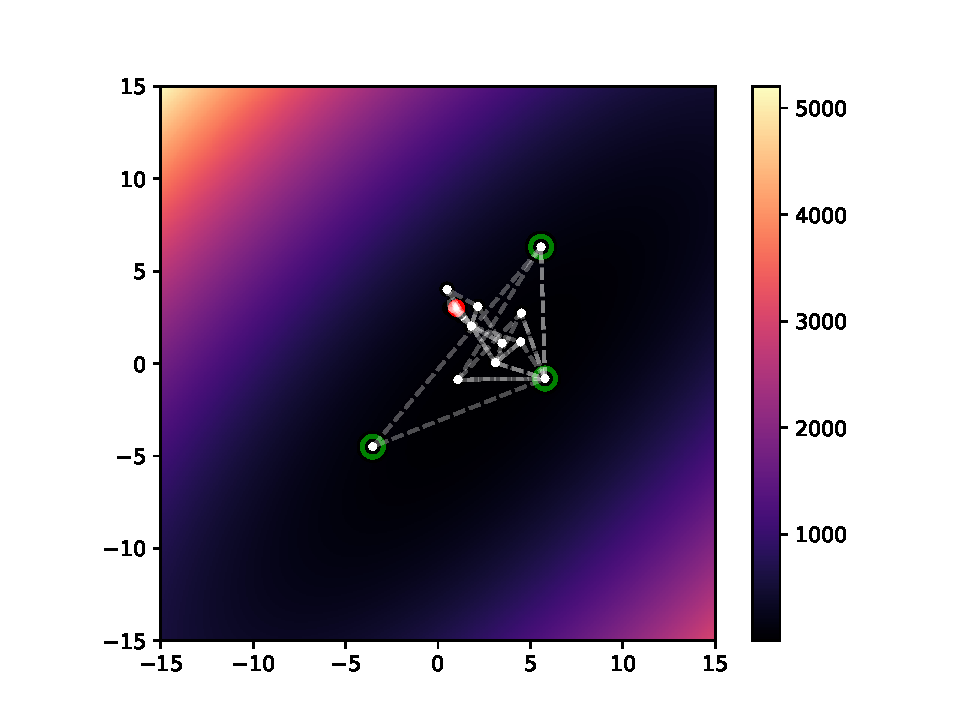
\includegraphics[width = .45\textwidth,trim={1cm 0 1cm 1cm}, clip]{Immagini/Booth3.pdf}}
	\subfloat[]{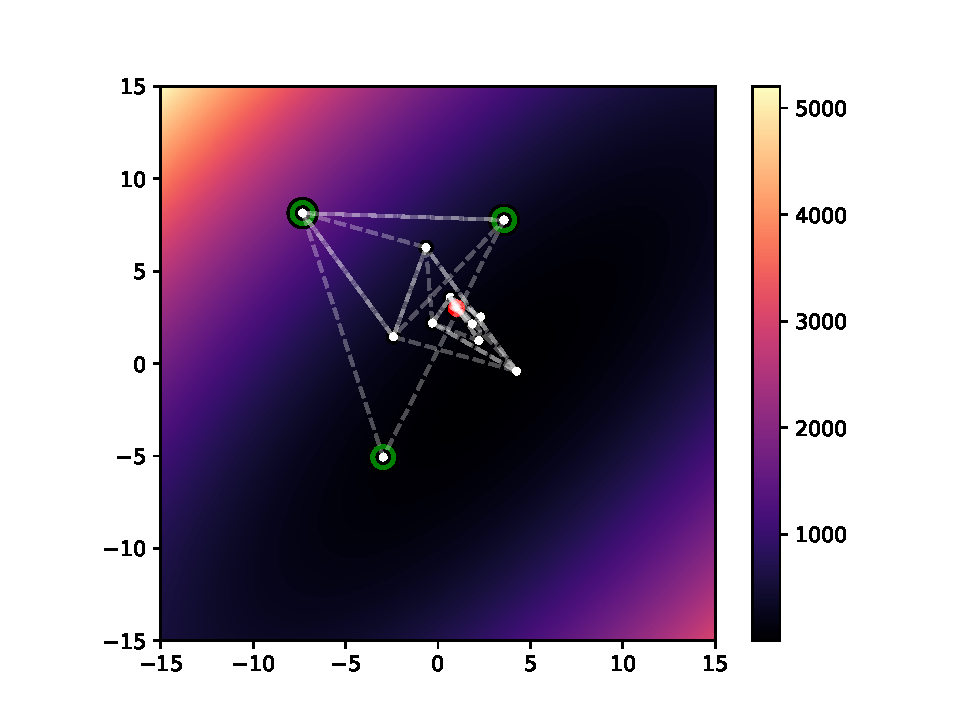
\includegraphics[width = .45\textwidth,trim={1cm 0 1cm 1cm}, clip]{Immagini/Booth4.pdf}} \\
	\subfloat[]{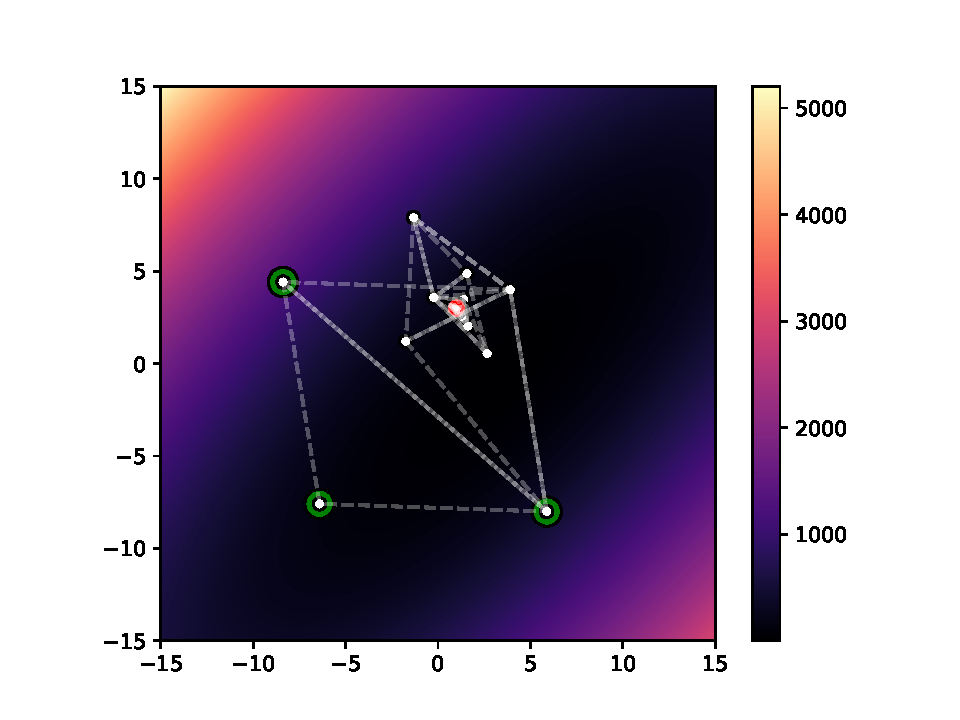
\includegraphics[width = .45\textwidth,trim={1cm 0 1cm 1cm}, clip]{Immagini/Booth5.pdf}}
	\subfloat[]{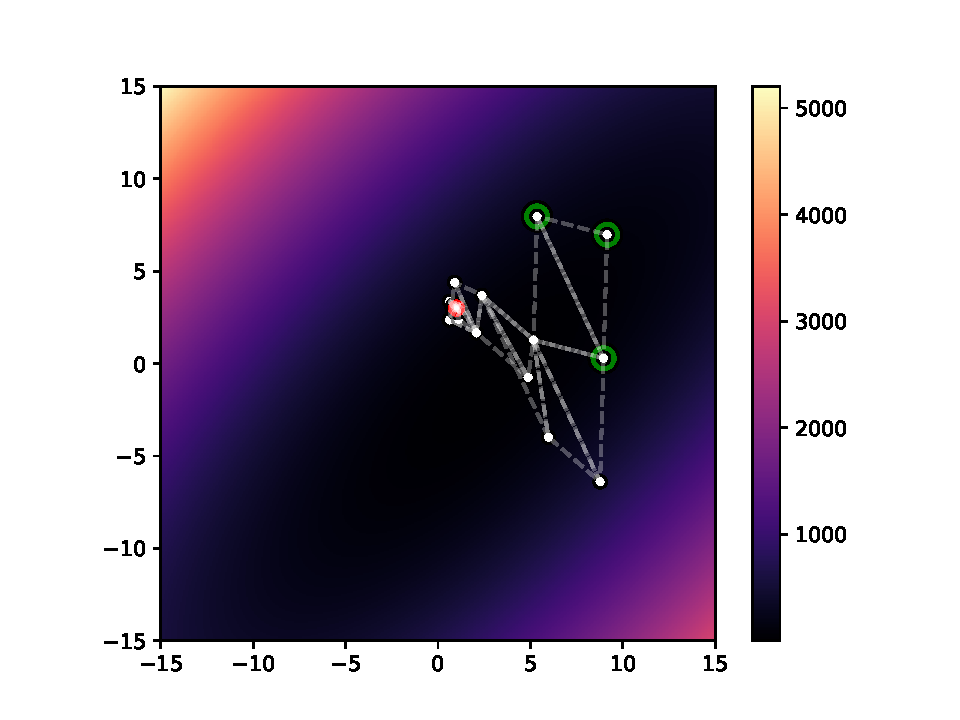
\includegraphics[width = .45\textwidth,trim={1cm 0 1cm 1cm}, clip]{Immagini/Booth6.pdf}}
	\label{fig:Booth}
\end{figure}

\newpage
\section{Esercizio 4}

Si calcoli con un metodo MC l'integrale $ \displaystyle\int_{-1}^{+1}(x^5+x^4)\mathop{dx}$ e si discutano le possibili tecniche di riduzione della varianza.

\bigskip\[* * * \] \smallskip

\noindent Consideriamo il generico integrale $ \displaystyle
\mathcal{S} = \int_a^b f(x) \mathop{dx}$, con $b>a \in \mathbb{R}$ e $f(x)$ funzione integrabile di variabile reale.\\

\noindent Definendo $g(x)$ come la densità di probabilità uniforme nell'intervallo $[a,b]$ possiamo riscrivere l'integrale $\mathcal{S}$ come

\begin{equation*}
(b-a)\int_{\mathbb{R}} f(x) g(x) \mathop{dx} = (b-a)\int_{\mathbb{R}}\mathbb{I}_{[a,b]}\frac{f(x)}{b-a}\mathop{dx} = \int_a^b f(x) \mathop{dx} = \mathcal{S},
\end{equation*}

\noindent e quindi definire un valore medio $F$ tale per cui $\mathcal{S} = (b-a)F$:

\begin{equation*}
F = \int_{\mathbb{R}}f(x)g(x)\mathop{dx}.
\end{equation*}

\noindent Per la \textit{legge dei grandi numeri} (Cfr.~\figurename~\ref{fig:MCHist}) possiamo inoltre costruire uno stimatore per $F$ utilizzando un generatore di numeri pseudo-casuali distribuiti secondo $g(x)$. Indicata con $\{x_i\}$ la sequenza generata e con $N$ la sua numerosità scriviamo allora:

\begin{equation}
\hat{F}_N = \frac{1}{N} \sum_{i=1}^{N}f(x_i),\quad \lim_{N\to\infty} (b-a)\hat{F}_N= \mathcal{S}.
\label{eq:MCstandard}
\end{equation}

\noindent Per $N$ finito possiamo anche valutare l'incertezza sulla stima di $\mathcal{S}$ per mezzo di uno stimatore della varianza di $\hat{F}_N$:

\begin{align}
\hat{S}_N &= \sqrt{\frac{1}{N-1} \left(\sum_{i=1}^{N}\bigl[(f(x_i))^2\bigr] - \bigl[\hat{F}_N\bigr]^2\right)}\\
\nonumber\\
\mathcal{S} &= (b-a)\left(\hat{F}_N \pm \frac{\hat{S}_N}{\sqrt{N}}\right)
\end{align}

\begin{figure}
	\centering
	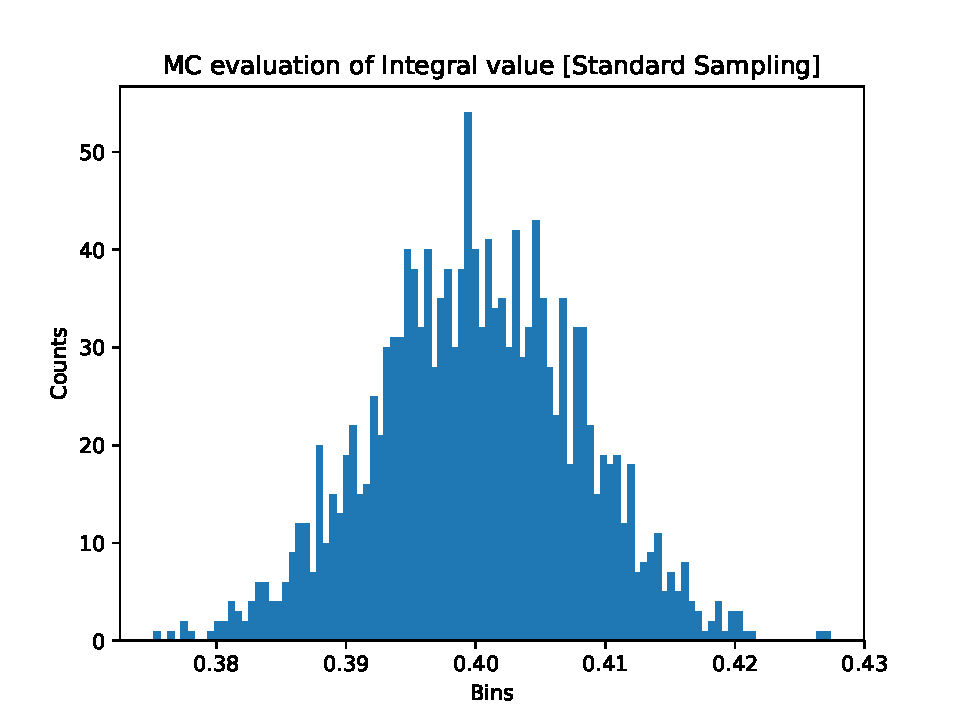
\includegraphics[width=.7\textwidth]{Immagini/Es4Hist.pdf}
	\caption{Istogramma relativo alla distribuzione generata per la variabile casuale $\mathcal{S}$ nell'implementazione standard del metodo Montecarlo, con $N=10^4$ eventi generati. \`E evidente che si tratta in buona approssimazione di una distribuzione normale, in accordo con la legge dei grandi numeri.}
	\label{fig:MCHist}
\end{figure}

\noindent Risulta subito evidente che la dipendenza da $N$ dell'incertezza non è particolarmente felice: pur garantendo uno stimatore non biassato nel limite $N\to\infty$, la convergenza è molto lenta producendo quindi algoritmi sostanzialmente inefficienti. Da tale considerazione nasce dunque l'interesse per algoritmi che riducano la varianza rispetto al metodo definito dalla (\ref{eq:MCstandard}), senza ovviamente produrre bias sul valor medio. Di seguito illustriamo due diverse tecniche di riduzione della varianza: \emph{Importance Sampling} e \emph{Stratified Sampling}.

\begin{description}
	
	\item[\quad\quad\! Importance Sampling]\quad\\
	Sia una generica densità di probabilità $p(x)\!: [a,b]\mapsto\mathbb{R}^+,\int_{a}^{b}p(x)\mathop{dx} = 1$. Se in $[a,b]$ tale densità si annulla al più in un sottoinsieme di punti di misura nulla possiamo riscrivere l'integrale $\mathcal{S}$ come:
	
	\begin{equation*}
	\mathcal{S} = \int_{a}^{b} \frac{f(x)}{p(x)}p(x)\mathop{dx} \simeq \frac{1}{N}\sum_{i=1}^{N}\frac{f(x_i)}{p(x_i)},\enspace \text{dove le } \{x_i\} \text{ sono distribuite secondo } p(x).
	\end{equation*}
	
	In questa situazione possiamo scrivere la varianza teorica di $\mathcal{S}$ come
	
	\begin{equation}
	\sigma^2[\,\mathcal{S}\,] = \frac{\sigma^2[\,f/p\,]}{N},
	\label{eq:ImportanceSampling}
	\end{equation}
	
	e osservare che laddove la densità $p(x)$ risulti proporzionale a $f(x)$ (in $[a,b]$!) la varianza $\sigma^2[\,f/p\,] = \sigma^2[\,\text{const.}]$ risulterà identicamente nulla. Senza pretese di rigore possiamo allora intuire che, fissato $N$, quanto più "$p(x)$ sarà simile a $f(x)$", tanto più la varianza di $\mathcal{S}$ tenderà a ridursi.\\
	Naturalmente nel caso generale risulta piuttosto difficile generare numeri casuali secondo una distribuzione simile alla funzione desiderata, per cui sostanzialmente si cerca di scrivere l'integrando come una combinazione lineare di densità note e si calcolano separatamente i rispettivi contributi a $\mathcal{S}$ e alla sua varianza. Nel nostro caso si è partizionato l'intervallo $[a,b]$ in maniera tale da poter approssimare la $f(x)$ con la somma di una distribuzione \emph{triangolare} e di una distribuzione \emph{beta}, con supporti disgiunti (Cfr.~\figurename~\ref{fig:MCImpSampl} e Listato~\ref{list:ImpSampling}).
		
	\item[\quad\quad\! Stratified Sampling]\quad\\
	Si tratta di un metodo basato sulla sola proprietà additiva degli integrali: considerato un punto $c\in[a,b]$ si ha analiticamente
	
	\begin{equation*}
	\int_{a}^{b} f(x)\mathop{dx} = \int_{a}^{c} f(x)\mathop{dx} + \int_{c}^{b} f(x)\mathop{dx}.
	\end{equation*}
	
	Tuttavia può essere dimostrato che partizionando l'intervallo $[a,b]$ in sottointervalli sui quali applicare un calcolo Montecarlo "standard" (i.e.~con estrazione di numeri casuali distribuiti uniformemente) si ottiene in generale una varianza totale differente rispetto al medesimo calcolo valutato sull'intervallo complessivo, a parità di estrazioni totali. In particolare si può allora ottimizzare la scelta di come ripartire nei sottointervalli il numero di eventi generati, al fine di minimizzare la varianza complessiva del calcolo: in ragione della (\ref{eq:ImportanceSampling}) possiamo argomentare che sarà preferibile campionare maggiormente le regioni in cui la funzione integranda varia più rapidamente, ossia laddove si discosti maggiormente da una densità uniforme. Nel nostro caso (Listato~\ref{list:StratSampling}) abbiamo definito sette sottointervalli con campionamento crescente da sinistra a destra, per un totale di $N$ eventi generati: in tal modo il calcolo risulta confrontabile con l'implementazione standard (Listato~\ref{list:MC}).
	
\end{description}

\noindent In linea di massima ci aspettiamo che l'\textit{Importance Sampling} risulti più efficiente nel ridurre la varianza rispetto allo\textit{ Stratified Sampling}, a patto che sia possibile approssimare la funzione integranda in combinazioni lineari di densità di probabilità elementari (i.e. semplici da generare). Nel caso generale invece un campionamento stratificato resta senz'altro l'opzione più flessibile e immediata da implementare.\\

\[* * * \] \smallskip

\noindent Di seguito riportiamo i risultati ottenuti con il calcolo \textit{Standard} (Listato~\ref{list:MC}), con\textit{ Importance Sampling} (Listato~\ref{list:ImpSampling}) e con \textit{Stratified Sampling} (Listato~\ref{list:StratSampling}), in termini di media e deviazione standard delle gaussiane generate per la variabile aleatoria $\mathcal{S}$. In tutti i casi sono stati estratti complessivamente $10^4$ campioni.
 
 \bgroup
 \def\arraystretch{2}
 \begin{center}
 	\begin{tabular}{r||c|c}
 	$ \mathcal{S} = \int_{-1}^{+1}(x^5+x^4)\mathop{dx}$ & \textit{Media Campionaria} & \textit{Deviazione Standard Campionaria }\\  \hline
 		\textit{Standard Sampling }& 0.4032560803645552  & 8.077310205890864 $\times \,\,10^{-3}$\\ 
 		\textit{Importance Sampling} & 0.3989493411116131 & 1.113214189831381 $\times\,\, 10^{-3}$\\ 
 		\textit{Stratified Sampling} & 0.4019606513273493 & 1.462526565299890 $\times \,\,10^{-3}$\\
 	\end{tabular}
 \end{center}
 \egroup
 
 \noindent Risulta innanzitutto evidente che i valori medi delle tre stime approssimano bene il valore analitico $\mathcal{S}=0.4$. Inoltre risultano tra loro compatibili ({entro meno di}~$2\sigma$), a riprova del fatto che le tecniche di riduzione della varianza utilizzate non traslano il valor medio dell'integrale. Osserviamo infine come la varianza campionaria diminuisce di un ordine di grandezza passando da \textit{Standard Sampling} a \textit{Stratified Sampling} e di quasi due ordini di grandezza utilizzando l'\textit{Importance Sampling}. Tali risultati soddisfano appieno le nostre aspettative.

\begin{figure}
	\centering
	\caption{Costruzione dell'\emph{Importance Sampling} per il calcolo di $\mathcal{S}$. Le due distribuzioni elementari utilizzate sono state moltiplicate per opportune costanti in modo da evidenziare quanto efficacemente riproducono la funzione~data.}
	\includegraphics[width=.77\textwidth, trim={0 .3cm 0 1.3cm},clip]{Immagini/Es4ImportanceSampling.pdf}
	\label{fig:MCImpSampl}
\end{figure}

\newpage

\begin{lstlisting}[language=python, style=Pystyle, caption=\texttt{Python} code for Standard Montecarlo Calculation, label=list:MC, 	captionpos=t]
import numpy as np
import matplotlib.pyplot as plt
import math

## Integrand function
def f(x): return x**5+x**4

## Integration interval
a =-1.0
b = 1.0

## Number of random number generations
n = 10000

## Standard MC implementation
h=[]
for k in range(1,1500):  

	x=np.random.uniform(a,b,n)  # [a,b]=[-1.0,1.0]
	eval_funct=f(x) 
	h.append((b-a)*np.sum(eval_funct)/(n))

S=(b-a)*(np.sum(eval_funct))/n
n=10000.0
mu_camp=(np.sum(eval_funct))/n
var_camp=1/(n-1)*np.sum((eval_funct-mu_camp)**2)
var=(b-a)**2*(1/n)*var_camp

print (S,'Integral Mean with Standard MC')
print (var,'Variance with Standard MC')
print(sqrt(var), 'Standard Deviation with Standard MC')

## Plotting a histogram of the generated gaussian
hist,bin_edges=np.histogram(h,bins=100)
plt.figure()
plt.hist(h,bin_edges)
plt.xlabel('Bins')
plt.ylabel('Counts')
plt.title('MC evaluation of Integral value [Standard Sampling]')
axes=plt.gca()

plt.show()
\end{lstlisting}

\begin{lstlisting}[language=python, style=Pystyle, caption=\texttt{Python} code for Importance Sampling Montecarlo Calculation, label=list:ImpSampling, 	captionpos=t]
import numpy as np
import matplotlib.pyplot as plt
import math
from scipy.stats import triang
from scipy.stats import beta

## Integrand function
def f(x): return x**5+x**4

x=np.linspace(-1,1,endpoint=True,dtype=float)
plt.plot(x,f(x),'.')

## 1st Interval: Triangular-approximation
s=np.linspace(-1,-0.25,50)
plt.plot(s,0.04*triang.pdf(s,0.2/0.7,a,b-a), '--')
a=-1
b=-0.25
n1=50
x1=np.random.triangular(a,-0.8,b,n1)  
eval_funct1=f(x1) 
y1=triang.pdf(x1,0.2/0.7,a,b-a)
n1=n1*1.0

i1=(1/n1)*np.sum(eval_funct1/y1)

mu_camp1=(np.sum(eval_funct1/y1))/n1
var_camp1=1/(n1-1)*np.sum((eval_funct1/y1-mu_camp1)**2)
var1=(1/n1)*var_camp1

## 2nd Interval: Beta-approximation
k=np.linspace(-0.25,1,100)
plt.plot(k,0.4*beta.pdf(k,5,1), '-.')

n2=9950
x2=beta.rvs(5,1,size=n2)  
eval_funct2=f(x2) 
y2=beta.pdf(x2,5,1)                     

n2=n2*1.0
i2=(1/n2)*np.sum(eval_funct2/y2)

mu_camp2=(np.sum(eval_funct2/y2))/n2
var_camp2=1/(n2-1)*np.sum((eval_funct2/y2-mu_camp2)**2)
var2=(1/n2)*var_camp2

## Results
print(i1+i2,'Integral Mean with Importance Sampling')
print(var1+var2,'Total Variance with Importance Sampling')
print(sqrt(var1+var2), 'Total Standard Deviation with Importance Sampling')
plt.xlabel('x')
plt.ylabel('y')
plt.show()
\end{lstlisting}

\begin{lstlisting}[language=python, style=Pystyle, caption=\texttt{Python} code for Stratified Sampling Montecarlo Calculation, label=list:StratSampling, 	captionpos=t]
import numpy as np
import math

## Integrand function
def f(x): return x**5+x**4

## 1st Interval 
a=-1.0
b=-0.4
n1=100
x1=np.random.uniform(a,b,n1)  # [a,b]=[-1.0,-0.4]
k=np.linspace(0.35,1,50)
eval_funct1=f(x1)
n1=n1*1.0 
i1=(b-a)*(np.sum(eval_funct1)/n1) # mean
mu_camp1=(np.sum(eval_funct1))/n1
var_camp1=(1/(n1-1))*np.sum((eval_funct1-mu_camp1)**2)  # variance
var1=(b-a)**2*(1/n1)*var_camp1

## 2nd Interval 
a=-0.4
b=0.4
n2=100
x2=np.random.uniform(a,b,n2)  # [a,b]=[-0.4,0.4]
eval_funct2=f(x2) 
n2=n2*1.0
i2=(b-a)*(np.sum(eval_funct2)/n2) # mean
mu_camp2=(np.sum(eval_funct2))/n2
var_camp2=1/(n2-1)*np.sum((eval_funct2-mu_camp2)**2)  # variance
var2=(b-a)**2*(1/n2)*var_camp2

## 3rd Interval 
a=0.4
b=0.6
n3=800
x3=np.random.uniform(a,b,n3)  # [a,b]=[0.4,0.6]
eval_funct3=f(x3) 
n3=n3*1.0
i3=(b-a)*(np.sum(eval_funct3)/n3) # mean
mu_camp3=(np.sum(eval_funct3))/n3
var_camp3=1/(n3-1)*np.sum((eval_funct3-mu_camp3)**2)  # variance
var3=(b-a)**2*(1/n3)*var_camp3

## 4th Interval 
a=0.6
b=0.7
n4=1000
x4=np.random.uniform(a,b,n4)  # [a,b]=[0.6,0.7]
eval_funct4=f(x4) 
n4=n4*1.0
i4=(b-a)*(np.sum(eval_funct4)/n4) # mean
mu_camp4=(np.sum(eval_funct4))/n4
var_camp4=1/(n4-1)*np.sum((eval_funct4-mu_camp4)**2)  # variance
var4=(b-a)**2*(1/n4)*var_camp4

## 5th Interval 
a=0.7
b=0.8
n5=1500
x5=np.random.uniform(a,b,n5)  # [a,b]=[0.7,0.8]
eval_funct5=f(x5) 
n5=n5*1.0
i5=(b-a)*(np.sum(eval_funct5)/n5) # mean
mu_camp5=(np.sum(eval_funct5))/n5
var_camp5=1/(n5-1)*np.sum((eval_funct5-mu_camp5)**2)  # variance
var5=(b-a)**2*(1/n5)*var_camp5

## 6th Interval 
a=0.8
b=0.9
n6=3000
x6=np.random.uniform(a,b,n6)  # [a,b]=[0.8,0.9]
eval_funct6=f(x6) 
n6=n6*1.0
i6=(b-a)*(np.sum(eval_funct6)/n6) # mean
mu_camp6=(np.sum(eval_funct6))/n6
var_camp6=1/(n6-1)*np.sum((eval_funct6-mu_camp6)**2)  # variance
var6=(b-a)**2*(1/n6)*var_camp6

## 7th Interval 
a=0.9
b=1.0
n7=3500
x7=np.random.uniform(a,b,n7)  # [a,b]=[0.9,1]
eval_funct7=f(x7) 
n7=n7*1.0
i7=(b-a)*(np.sum(eval_funct7)/n7) # mean
mu_camp7=(np.sum(eval_funct7))/n7
var_camp7=1/(n7-1)*np.sum((eval_funct7-mu_camp7)**2)  # variance
var7=(b-a)**2*(1/n7)*var_camp7

## Results
print(n1+n2+n3+n4+n5+n6+n7,'Check on total number of generations [has to be 10^4]')
S=i1+i2+i3+i4+i5+i6+i7
print(S,'Total mean for S, with Stratified Sampling')
var=var1+var2+var3+var4+var5+var6+var7
print(var ,'Total variance for S, with Stratified Sampling')
dev = sqrt(var)
print(dev ,'Total standard deviation for S, with Stratified Sampling')
\end{lstlisting}

\newpage
\section{Esercizio 5}

\begin{enumerate}[label=\Alph*.]
	
	\item Nel dropbox del corso sono presenti alcuni files di dati del tipo \texttt{CeBr3\_xx.dat} con \texttt{xx} nome di una sorgente di calibrazione: $\mathrm{Cs}^{137}$, $\mathrm{Co}^{57}$, $\mathrm{Na}^{22}$, $\mathrm{Ba}^{133}$ e $\mathrm{Eu}^{152}$.\\
	I dati sono lo spettro in formato ASCII di un MCA (con 8K canali) per un cristallo di $\mathrm{CeBr}_3$ esposto a varie sorgenti di calibrazione. Istogrammare i vari spettri di multicanale e scrivere un programma per determinare posizione e risoluzione spettrale dei picchi di calibrazione, il più automatizzato possibile.\\
	Si discutano i risultati ottenuti in termini di risoluzione energetica del cristallo e linearità.
	\item Utilizzando gli algoritmi di smoothing illustrati a lezione, provare a vedere se si riesce a migliorare la determinazione spettrale dei picchi spettrali trovati: area, altezza... Discutere i risultati ottenuti. 
	
\end{enumerate}

\[* * * \] \smallskip

\noindent In \figurename~\ref{fig:RAW} sono riportati i grafici dei dati, così come riportati nei file di input relativi all'esposizione del cristallo alle diverse sorgenti (conteggi "grezzi"). Per individuarne in maniera automatizzata i picchi di risonanza si è pensato innanzitutto di dividere il dominio spettrale dell'analizzatore multicanale in sotto-bande sulle quali determinare il massimo assoluto dei conteggi: scegliendo opportunamente la larghezza di queste regioni di ottimizzazione locale si ha buona speranza di individuare un sottoinsieme di canali che includa tutti i bin contenenti le frequenze di risonanza cercate. Naturalmente alcuni dei massimi così individuati saranno solo artefatti della suddivisione operata sulla banda del rivelatore (ad esempio valori al bordo di una sotto-banda in cui lo spettro è monotono) per cui rigettiamo tutti quelli che non soddisfino le condizioni elementari che definiscono un punto stazionario di massimo:

\newcounter{conditions}
\begin{enumerate}
\item derivata prima dei conteggi compresa in un piccolo intorno dello zero;
\item derivata seconda dei conteggi minore di una certa soglia negativa.
\setcounter{conditions}{\value{enumi}}
\end{enumerate}

\noindent A questo punto si saranno certamente individuati dei massimi locali dell'intero spettro che siano anche ottimi globali nelle rispettivi sotto-regioni di ricerca.\\

\noindent Resta tuttavia qualche criticità su eventuali \emph{plateau} degli spettri analizzati: mancando nelle sotto-regioni interessate dei picchi "veri", le oscillazioni riconducibili al rumore intrinseco della rivelazione danno inevitabilmente luogo a \emph{falsi positivi} (ossia massimi locali non associati a risonanze del cristallo scintillatore). Per ovviare a tal problema è stata definita un'ulteriore condizione necessaria per l'accettazione dei valori selezionati:

\begin{enumerate}
	\setcounter{enumi}{\value{conditions}}
	\item  numero di conteggi maggiore di una certa soglia, associabile ai picchi di rumore.
\end{enumerate}

\noindent Naturalmente tutta la difficoltà di implementazione dell'algoritmo risiede nella definizione dei parametri per le condizioni (1), (2) e (3), considerate soprattutto la richiesta di massima automazione della routine e la conseguente sconvenienza di un'accordatura manuale da operare di volta in volta sulla base dei dati analizzati. Si è scelto di far dipendere opportunamente tali parametri dalla sotto-banda di origine del candidato picco e in particolare di~considerare:

\begin{itemize}
	\item[-] << \texttt{a = 1.10 * mean\{Counts on Sub-Region\}} >> come soglia sui conteggi $(\,y > a\,)$;
	\item[-] << \texttt{b = 0.45 * max\{Derivative - Counts on Sub-Region\}} >> come soglia sulla pendenza $(\,|y'|<b\,)$;
	\item[-] << \texttt{c = 0.05 * max\{2ndDerivative - Counts on Sub-Region\}} >> come soglia sulla concavità $(\,y'' < -c\,)$.
\end{itemize}

\noindent Le derivate dei conteggi sono state valutate numericamente per mezzo di differenze finite al secondo ordine, utilizzando la libreria \texttt{numpy.gradient} di~\texttt{Python}\footnote{Documentazione consultabile al seguente link: \href{https://docs.scipy.org/doc/numpy-1.15.0/reference/generated/numpy.gradient.html}{\texttt{https://docs.scipy.org/doc/[...]/numpy.gradient.html}}}.\\

\noindent Infine, per assicurarsi di eliminare qualsiasi artefatto ancora dovuto al particolare partizionamento dello spettro, si è pensato di ripetere l'intera procedura con una differente scelta per la larghezza dei sotto-intervalli e di accettare definitivamente soltanto i candidati picchi individuati da entrambe le istanze della routine. In particolare, definito innanzitutto il range effettivo dei dati considerati (tutti gli spettri hanno una soglia energetica oltre la quale sono sostanzialmente nulli), l'intervallo risultante è stato suddiviso la prima volta in  20 e la seconda in 8 parti uguali, sulle quali sono stati definiti i candidati picchi, poi filtrati secondo le condizioni (1), (2) e (3). Il confronto diretto tra i due \emph{data-set} così ottenuti ha decretato quali candidati accettare come effettivi picchi di risonanza.\\

\noindent  In \figurename~\ref{fig:PeakSearchRaw} sono indicati (\textit{croci arancioni}) i punti che l'algoritmo proposto ha individuato sugli spettri: risulta subito evidente che qualche picco importante non è stato individuato, soprattutto su  Co$^{57}$ e Na$^{22}$. D'altra parte ci riteniamo soddisfatti dal grado di selettività della routine rispetto ai falsi positivi, considerato l'alto livello di rumore presentato da alcuni degli spettri proposti. I dettagli dell'implementazione in \texttt{Python} possono essere consultati nella prima parte del Listato~\ref{list:PeakRoutine}.\\

\noindent Per indagare la risoluzione energetica del cristallo scintillatore abbiamo deciso di analizzare per ogni spettro il Picco Principale (P.P.), inteso come quello relativo alla risonanza che ha prodotto più conteggi sul rivelatore: la strategia è mirata alla minimizzazione dei problemi dovuti al rumore delle misure.\\

\noindent Innanzitutto è stato necessario definire una \texttt{ROI} (\texttt{Region Of Interest}) attorno al P.P. in modo da poter operare un \emph{fitting} parametrico dei conteggi relativi alla sola risonanza considerata. Si è assunto che il picco abbia profilo simil-Gaussiano, al netto di un eventuale fondo da sottrarre opportunamente. In particolare la \texttt{ROI} attorno al picco è stata definita come il \underline{minimo} intorno del punto di massimo tale da soddisfare le seguenti condizioni, scelte in modo da funzionare robustamente per tutti gli spettri proposti:

\begin{align*}
\Bigl|y_\texttt{ROI} - y_\mathrm{max}\Bigr| &\leq \frac{3}{4} \times y_\mathrm{max}, \\
\\
\Bigl|y'_\texttt{ROI}\Bigr| &< 50.
\end{align*}

\noindent Il fondo è stato approssimato al segmento congiungente i due punti spettrali agli estremi della \texttt{ROI}, per mezzo della libreria \texttt{Python} adibita all'interpolazione polinomiale con metodo l.s.~\!(\emph{least squares}): \texttt{numpy.polyfit}\footnote{Documentazione: \href{https://docs.scipy.org/doc/numpy-1.15.0/reference/generated/numpy.polyfit.html}{\texttt{https://docs.scipy.org/doc/[...]/numpy.polyfit.html}}}. Infine anche il fit Gaussiano è stato ottenuto con metodo l.s., ma adoperando la più generica libreria \texttt{scipy.optimize.curve\_fit}\footnote{Documentazione: \href{https://docs.scipy.org/doc/scipy/reference/generated/scipy.optimize.curve_fit.html}{\texttt{https://docs.scipy.org/doc/[...]/scipy.optimize.curve\_fit.html}}} che permette di definire a piacere il modello da adattare ai dati.

\vfill

\noindent A partire dunque dalla definizione:

\vfill

\begin{equation*}
g(x) = A\,\exp\!\left[\frac{-(x-x_0)^2}{2\sigma^2}\right],
\end{equation*}
 
 \vfill
 
\noindent e fornendo al \emph{fitter} i parametri iniziali:

\vfill

\begin{equation*}
A\,\Bigr|^\mathrm{init} = y_\mathrm{max},\quad x_0\,\Bigr|^\mathrm{init} = x_\mathrm{max},\quad \sigma\,\Bigr|^\mathrm{init} = \hat{\sigma}_x(\texttt{DATA}),
\end{equation*}

\vfill

\noindent otteniamo i risultati\footnote{Larghezza del picco $w$ e relativa risoluzione spettrale $w/x_0$ sono calcolate come da standard \texttt{FWHM}. L'area sottesa è stimata in approssimazione triangolare $S\simeq wA/2$. Le incertezze infine sono ricavate dalla matrice di covarianza restituita dal \emph{fitter}} riportati nelle Figure~\ref{fig:PPRawCs137},~\ref{fig:PPRawCo57},~\ref{fig:PPRawNa22},~\ref{fig:PPRawBa133}~e~\ref{fig:PPRawEu152}.\\

\vfill

\begin{sidewaysfigure}
	\centering
	\caption{Istogrammi grezzi dei cinque spettri di calibrazione considerati.}
	\subfloat{\includegraphics[width = .33\textwidth,trim={.1cm 0 1cm 0}, clip]{Immagini/RawCs137.pdf}} 
	\subfloat{\includegraphics[width =  .33\textwidth,trim={.1cm 0 1cm 0}, clip]{Immagini/RawCo57.pdf}}
	\subfloat{\includegraphics[width = .33\textwidth,trim={.1cm 0 1cm 0}, clip]{Immagini/RawNa22.pdf}}\\
	\subfloat{\includegraphics[width = .33\textwidth,trim={.1cm 0 1cm 0}, clip]{Immagini/RawBa133.pdf}}
	\subfloat{\includegraphics[width = .33\textwidth,trim={.1cm 0 1cm 0}, clip]{Immagini/RawEu152.pdf}}
	\label{fig:RAW}
\end{sidewaysfigure}

\begin{sidewaysfigure}
	\centering
	\caption{Ricerca dei picchi di scintillazione sugli spettri di calibrazione grezzi.}
	\subfloat{\includegraphics[width = .33\textwidth,trim={.1cm 0 1cm 0}, clip]{Immagini/RawCs137_with_determined_peaks.pdf}} 
	\subfloat{\includegraphics[width =  .33\textwidth,trim={.1cm 0 1cm 0}, clip]{Immagini/RawCo57_with_determined_peaks.pdf}}
	\subfloat{\includegraphics[width = .33\textwidth,trim={.1cm 0 1cm 0}, clip]{Immagini/RawNa22_with_determined_peaks.pdf}}\\
	\subfloat{\includegraphics[width = .33\textwidth,trim={.1cm 0 1cm 0}, clip]{Immagini/RawBa133_with_determined_peaks.pdf}}
	\subfloat{\includegraphics[width = .33\textwidth,trim={.1cm 0 1cm 0}, clip]{Immagini/RawEu152_with_determined_peaks.pdf}}
	\label{fig:PeakSearchRaw}
\end{sidewaysfigure}

\newpage

\begin{lstlisting}[language=python, style=Pystyle, caption=\texttt{Python} code for Spectral Peak Recognition Routine, label=list:PeakRoutine, 	captionpos=t]
""" Standard Libraries """
import numpy as np
import pylab as plt
from math import *

""" I/O Libraries """
import os
import sys

""" Best-Fit Library """
from scipy.optimize import curve_fit

########################################################################################

## Choosing the source

SourceName = str(input('Insert the desired source [Cs137|Co57|Na22|Ba133|Eu152]: '))

## Opening the ASCII file related to the chosen source

def get_script_path():
	return os.path.dirname(os.path.realpath(sys.argv[0]))

path = get_script_path()
data=np.loadtxt(path+'/Script&Data/CeBr3_'+SourceName+'.dat')

## Defining Effective-Range

i = len(data)
while(data[i-1] <= 0.01*np.max(data)/2): 
i = i - 1

x_max = i
data = data[range(1,x_max)]

## Plotting retrieved experimental data

x = np.array(range(1,x_max))
y = data

plt.figure('Raw'+SourceName)
plt.plot(x,y,'ko',markersize=0.5)
plt.xlim((1, x_max))
plt.xlabel('Channels')
bottom, top = plt.ylim()
plt.ylabel('Counts')
plt.title('RAW Data ['+SourceName+']')
plt.ticklabel_format(axis='both',style='sci',scilimits=(0,0),useMathText=True)
plt.show()

##############################
## Peak-Recognition Routine ##
##############################

# Derivatives of data
y1 = np.gradient(y)
y2 = np.gradient(y1)

X_Peaks1 = np.array([])
Y_Peaks1 = np.array([])
X_Peaks2 = np.array([])
Y_Peaks2 = np.array([])
Y1 = np.array([])
Y2 = np.array([])

steps = 20
for i in range(1,steps+1):
	
	# Minimization only in a partial domain
	X = x[(x > (x_max/steps)*(i-1)) & (x <= (x_max/steps)*i)]
	Y = y[(x > (x_max/steps)*(i-1)) & (x <= (x_max/steps)*i)]
	Y1 = y1[(x > (x_max/steps)*(i-1)) & (x <= (x_max/steps)*i)]
	Y2 = y2[(x > (x_max/steps)*(i-1)) & (x <= (x_max/steps)*i)]
	X_CandidatePeak = X[np.argmax(Y)]
	Y_CandidatePeak = np.max(Y)
	Y1_CandidatePeak = Y1[np.argmax(Y)]
	Y2_CandidatePeak = Y2[np.argmax(Y)]
	
	a = 1.1*np.max(Y)/2         # Threshold on Background
	b = 0.9*np.max(abs(Y1))/2   # Threshold on Slope
	c = 0.1*np.max(abs(Y2))/2   # Threshold on Concavity
	
	if (Y_CandidatePeak > a)and(abs(Y1_CandidatePeak)< b)and(Y2_CandidatePeak<-c)and(Y_CandidatePeak > 0.13*np.max(y)):
	
		X_Peaks1 = np.append(X_Peaks1, X_CandidatePeak)
		Y_Peaks1 = np.append(Y_Peaks1, Y_CandidatePeak)
	
steps = 8
for i in range(1,steps+1):
	
	# Minimization only in a partial domain
	X = x[(x > (x_max/steps)*(i-1)) & (x <= (x_max/steps)*i)]
	Y = y[(x > (x_max/steps)*(i-1)) & (x <= (x_max/steps)*i)]
	Y1 = y1[(x > (x_max/steps)*(i-1)) & (x <= (x_max/steps)*i)]
	Y2 = y2[(x > (x_max/steps)*(i-1)) & (x <= (x_max/steps)*i)]
	X_CandidatePeak = X[np.argmax(Y)]
	Y_CandidatePeak = np.max(Y)
	Y1_CandidatePeak = Y1[np.argmax(Y)]
	Y2_CandidatePeak = Y2[np.argmax(Y)]
	
	a = 1.1*np.max(Y)/2         # Threshold on Background
	b = 0.9*np.max(abs(Y1))/2   # Threshold on Slope
	c = 0.1*np.max(abs(Y2))/2   # Threshold on Concavity
	
	if (Y_CandidatePeak > a)and(abs(Y1_CandidatePeak)< b)and(Y2_CandidatePeak<-c)and(Y_CandidatePeak > 0.13*np.max(y)):
	
		for j in range(len(X_Peaks1)):
			if X_CandidatePeak == X_Peaks1[j]:
				X_Peaks2 = np.append(X_Peaks2, X_CandidatePeak)
				Y_Peaks2 = np.append(Y_Peaks2, Y_CandidatePeak)

# Showing determined peaks
plt.figure('Raw'+SourceName+' with determined peaks')
plt.plot(x,y,'ko',markersize=0.5)
plt.xlim((1, x_max))
plt.xlabel('Channels')
bottom, top = plt.ylim()
plt.ylabel('Counts')
plt.title('RAW Data with determined peaks ['+SourceName+']')
plt.ticklabel_format(axis='both',style='sci',scilimits=(0,0),useMathText=True)
plt.show()
plt.plot(X_Peaks2,Y_Peaks2,'X',c='orange',markeredgecolor='k',markersize=10,alpha=0.75)

## Principal-Peak [P.P] Analysis

xmax_peak = X_Peaks2[np.argmax(Y_Peaks2)]   # Principal-Peak position
ymax_peak = np.max(Y_Peaks2)                # Principal-Peak value
index = np.where(x==xmax_peak)[0]           # Finding P.P in our data array

########################################################################################
# Definition of a ROI: we must have |yROI-yPeak|<=d and |yROI'|<t, on both sides of P.P.
########################################################################################
d = ymax_peak*0.75 # -----------------------
t = 50             # BEST VALUES [HEURISTIC]
#################### -----------------------

x1=x[(abs(y1)<t) & (x<xmax_peak) & (abs(y-ymax_peak)>d)]
index1=np.where(x==x1[abs(x1-xmax_peak)==min(abs(x1-xmax_peak))])[0]
i1=np.array(index1[0])
x2=x[(abs(y1)<t) & (x>xmax_peak) & (abs(y-ymax_peak)>d)]
index2=np.where(x==x2[abs(x2-xmax_peak)==min(abs(x2-xmax_peak))])[0]
i2=np.array(index2[0])
xnew=x[i1:i2]
ynew=y[i1:i2]

#Plotting the ROI-confined Peak
plt.figure('Peak-Fitting_'+SourceName)
plt.plot(x[range(i1-1,i2+1)],y[range(i1-1,i2+1)],'ko',markersize=1.5,label='ROI-data')

# Background Esimate: Linear-Fit beetwen ROI edges... 
a=xnew[0]
b=xnew[len(xnew)-1]
x_to_fit = np.array([xnew[0],xnew[len(xnew)-1]])
y_to_fit = np.array([ynew[0],ynew[len(xnew)-1]])
coefficients = np.polyfit(x_to_fit, y_to_fit, deg=1) # Linear-Fit
polynomial = np.poly1d(coefficients)                 # ----------
x_pol = np.linspace(xnew[0],xnew[len(xnew)-1],100)
y_pol = polynomial(x_pol)
plt.plot(x_pol,y_pol,'m-.',linewidth=1.5,alpha=0.5,label='Background')

# Background-correcting the Peak [and plotting]
ynew=ynew-polynomial(xnew)
plt.plot(xnew,ynew,'o',c='orange',markersize=1.5,label='Corrected-Peak')
plt.ylim(0,ymax_peak*2-1.25*d)

## Gaussian Best-Fit of the corrected P.P. data

def Gauss(x,A,x0,sigma):
return A*np.exp(-(x-x0)**2/(2*sigma**2))

A_init = np.max(ynew)       # -----------
x0_init = np.mean(xnew)     # First guess
sigma_init = np.std(xnew)   # -----------

# Least-Squares Fitting...
popt,pcov = curve_fit(Gauss,xnew,ynew,p0=[A_init,x0_init,sigma_init])

A = popt[0]                                  # ----------------
x0 = popt[1]                                 # Best-Fit results
sigma = popt[2]                              # ----------------
StDev_vec = 2.3548200*np.sqrt(np.diag(pcov)) # ----------------

W = 2.3548200*popt[2] # Peak-Width: FWHM
S = 0.5*A*W # Area with Triangle-Approx.
R = W/x0 # Resolution: FWHM/x0

dA = StDev_vec[0]
dx = StDev_vec[1]
dW = 2.3548200*StDev_vec[2]
dS = (dA/A + dW/W)*S
dR = (dW/W + dx/x0)*R

# Printing Results...
print('PRINCIPAL-PEAK POSITION', x0,''"$\pm$", dx)
print('PRINCIPAL-PEAK HEIGHT: ', A,''"$\pm$", dA)
print('PRINCIPAL-PEAK WIDTH: ', W,''"$\pm$", dW)
print('PRINCIPAL-PEAK AREA :', S,''"$\pm$", dS)
print('CRYSTAL RESOLUTION: ', R,''"$\pm$", dR)

# Plotting & Showing All
yFIT = Gauss(xnew,A,x0,sigma)
plt.plot(xnew,yFIT,'g--',linewidth=1.5,label='Gaussian-Fit')
plt.title('Principal Peak Best-Fitting ['+SourceName+']')
plt.ticklabel_format(axis='both',style='sci',scilimits=(0,0),useMathText=True)
plt.legend(markerscale=3)
plt.show()
\end{lstlisting}

\begin{figure}[h!]
	\centering
	\caption{Analisi su dati grezzi del Picco Principale (P.P.) della sorgente Cs$^{137}$. }
	\includegraphics[width =  \textwidth,trim={1cm 0 1cm 0}, clip]{Immagini/Peak-Fitting_Cs137_RAW.pdf}
	\label{fig:PPRawCs137} \bigskip\bigskip
	\begin{lstlisting}[language=python, style=Pystyle, mathescape=true]
	>>> (executing file "PhytonCodeEs5.py")
	Insert the desired source [Cs137|Co57|Na22|Ba133|Eu152]: Cs137
	PRINCIPAL-PEAK POSITION 238.8467517967467 $\pm$ 0.3098839895739907
	PRINCIPAL-PEAK HEIGHT:  1523.3400945401845 $\pm$ 26.00320803587605
	PRINCIPAL-PEAK WIDTH:  37.09865495020793 $\pm$ 0.7485587193418013
	PRINCIPAL-PEAK AREA : 28256.934269581718 $\pm$ 1052.4967764062292
	CRYSTAL RESOLUTION:  0.15532409241963677 $\pm$ 0.003335574642671817
	\end{lstlisting} \bigskip\bigskip
\end{figure}

\newpage

\begin{figure}[h!]
	\centering
	\caption{Analisi su dati grezzi del Picco Principale (P.P.) della sorgente Co$^{57}$. }
	\includegraphics[width =  \textwidth,trim={1cm 0 1cm 0}, clip]{Immagini/Peak-Fitting_Co57_RAW.pdf}
	\label{fig:PPRawCo57} \bigskip\bigskip
	\begin{lstlisting}[language=python, style=Pystyle, mathescape=true]
	>>> (executing file "PhytonCodeEs5.py")
	Insert the desired source [Cs137|Co57|Na22|Ba133|Eu152]: Co57
	PRINCIPAL-PEAK POSITION 693.1137861569199 $\pm$ 0.4433360809406253
	PRINCIPAL-PEAK HEIGHT:  148880.4511121081 $\pm$ 1769.474256713379
	PRINCIPAL-PEAK WIDTH:  76.09652174560256 $\pm$ 1.04632416144232
	PRINCIPAL-PEAK AREA : 5664642.242773826 $\pm$ 145214.0247096522
	CRYSTAL RESOLUTION:  0.10978936397663056 $\pm$ 0.0015798239331929512
	\end{lstlisting} \bigskip\bigskip
\end{figure}

\newpage

\begin{figure}[h!]
	\centering
	\caption{Analisi su dati grezzi del Picco Principale (P.P.) della sorgente Na$^{22}$. }
	\includegraphics[width =  \textwidth,trim={1cm 0 1cm 0}, clip]{Immagini/Peak-Fitting_Na22_RAW.pdf}
	\label{fig:PPRawNa22} \bigskip\bigskip
	\begin{lstlisting}[language=python, style=Pystyle, mathescape=true]
	>>> (executing file "PhytonCodeEs5.py")
	Insert the desired source [Cs137|Co57|Na22|Ba133|Eu152]: Na22
	PRINCIPAL-PEAK POSITION 2679.8233949851183 $\pm$ 1.0636289671764676
	PRINCIPAL-PEAK HEIGHT:  644.6055128147791 $\pm$ 9.837826754288718
	PRINCIPAL-PEAK WIDTH:  142.39273009203848 $\pm$ 2.6530917116409816
	PRINCIPAL-PEAK AREA : 45893.56940103744 $\pm$ 1555.5162765213215
	CRYSTAL RESOLUTION:  0.05313511717171542 $\pm$ 0.0010111143019759258
	\end{lstlisting} \bigskip\bigskip
\end{figure}

\newpage

\begin{figure}[h!]
	\centering
	\caption{Analisi su dati grezzi del Picco Principale (P.P.) della sorgente Ba$^{133}$. }
	\includegraphics[width =  \textwidth,trim={1cm 0 1cm 0}, clip]{Immagini/Peak-Fitting_Ba133_RAW.pdf}
	\label{fig:PPRawBa133} \bigskip\bigskip
	\begin{lstlisting}[language=python, style=Pystyle, mathescape=true]
	>>> (executing file "PhytonCodeEs5.py")
	Insert the desired source [Cs137|Co57|Na22|Ba133|Eu152]: Ba133
	PRINCIPAL-PEAK POSITION 221.25212247553907 $\pm$ 1.2732933530258672
	PRINCIPAL-PEAK HEIGHT:  287864.93020777084 $\pm$ 12741.050893987342
	PRINCIPAL-PEAK WIDTH:  58.70101313148694 $\pm$ 3.0122036998891812
	PRINCIPAL-PEAK AREA : 8448981.524110464 $\pm$ 807510.2018385414
	CRYSTAL RESOLUTION:  0.2653127684141278 $\pm$ 0.01514120925440681
	\end{lstlisting} \bigskip\bigskip
\end{figure}

\newpage

\begin{figure}[h!]
	\centering
	\caption{Analisi su dati grezzi del Picco Principale (P.P.) della sorgente Eu$^{152}$. }
	\includegraphics[width =  \textwidth,trim={1cm 0 1cm 0}, clip]{Immagini/Peak-Fitting_Eu152_RAW.pdf}
	\label{fig:PPRawEu152} \bigskip\bigskip
	\begin{lstlisting}[language=python, style=Pystyle, mathescape=true]
	>>> (executing file "PhytonCodeEs5.py")
	Insert the desired source [Cs137|Co57|Na22|Ba133|Eu152]: Eu152
	PRINCIPAL-PEAK POSITION 289.67056608195855 $\pm$ 0.15968983090396094
	PRINCIPAL-PEAK HEIGHT:  149000.1993161386 $\pm$ 887.0254434869172
	PRINCIPAL-PEAK WIDTH:  54.704433482585735 $\pm$ 0.3760595236985809
	PRINCIPAL-PEAK AREA : 4075485.7461908604 $\pm$ 52278.58417820594
	CRYSTAL RESOLUTION:  0.18885050774232898 $\pm$ 0.0014023414074840683
	\end{lstlisting} \bigskip\bigskip
\end{figure}

\newpage

\noindent Complessivamente l'analisi operata sui dati grezzi risulta ragionevole: i valori di incertezza sui parametri di \emph{best-fit} sono almeno di due ordini di grandezza inferiori al relativo valore stimato in tutti casi meno che per il P.P del Ba$^{133}$, che ha profilo palesemente non gaussiano. Osserviamo che la risoluzione spettrale dei picchi risulta migliore per le risonanze a energie inferiori, per cui deduciamo che il cristallo abbia risoluzione decrescente con l'energia di eccitazione: di ciò abbiamo trovato riscontro in letteratura\footnote{\href{http://www.sympnp.org/proceedings/62/G51.pdf}{G. Mishra \emph{et al.}, Proc. \!DAE Symp. \!\!Nucl. \!\!Phys. \!\!62 (2017) 1092-1093\\ \href{https://doi.org/10.1016/j.nima.2013.08.005}{F. Quarati \emph{et al.}, Nuclear Instruments and Methods in Physics Research A 729 (2013) 596–604}}}. Per quanto riguarda le proprietà di risposta del cristallo abbiamo invece confrontato direttamente gli istogrammi grezzi in \figurename~\ref{fig:RAW} con gli spettri di emissione riportati su \href{https://www.gammaspectacular.com}{\texttt{Gamma \!\!Spectacular}} per alcune delle sorgenti considerate\footnote{In particolare per Na$^{22}$ e Ba$^{133}$ riconoscendone i picchi rispettivamente a 511~keV e 1274~kev e a 31~keV e 81~keV.} e dedotto che il cristallo non presenta una buona linearità se non nel limite di alte energie.

\[* * * \] \smallskip

\noindent Per operare lo {smoothing} dei dati si è adoperata la libreria \texttt{scipy.ndimage.gaussian\_filter}\footnote{Documentazione: \href{https://docs.scipy.org/doc/scipy/reference/generated/scipy.ndimage.gaussian_filter.html}{\texttt{https://docs.scipy.org/doc/scipy/reference/generated/scipy.ndimage.gaussian\_filter.html}}} di \texttt{Python}, ottenendo i risultati riportati in \figurename~\ref{fig:Smoothing} secondo il codice di seguito riportato:

\vfill

\begin{lstlisting}[language=python, style=Pystyle, caption=\texttt{Python} code for Gaussian Smoothing Routine, label=list:Smoothing, 	captionpos=b]
""" Gaussian-Smoothing Library """
from scipy.ndimage import gaussian_filter as smoothing

## Smoothing Data
y=smoothing(data,sigma=5)

## Plotting Results
plt.figure('Smoothing'+SourceName)
plt.plot(x,data,'ko',markersize=0.5,label='RAW Data')
plt.plot(x,y,'ro',markersize=0.5,label='Smoothed')
plt.xlim((1, x_max))
plt.xlabel('Channels')
plt.ylim((bottom, top))
plt.ylabel('Counts')
plt.title('Smoothing ['+SourceName+']')
plt.legend(markerscale=10)
plt.ticklabel_format(axis='both',style='sci',scilimits=(0,0),useMathText=True)
plt.figure('Smoothed'+SourceName)
plt.plot(x,y,'ro',markersize=0.5)
plt.xlim((1, x_max))
plt.xlabel('Channels')
plt.ylim((bottom, top))
plt.ylabel('Counts')
plt.title('Smoothed Data with determined peaks ['+SourceName+']')
plt.ticklabel_format(axis='both',style='sci',scilimits=(0,0),useMathText=True)
plt.show()
\end{lstlisting}

\vfill

\noindent L'applicazione della medesima routine (Listato~\ref{list:PeakRoutine} a partire dalla riga 50) sui dati sottoposti a smoothing porta a individuare i picchi riportati in \figurename~\ref{fig:PeakSearchSmoothed}, in cui possiamo osservare come le risonanze trascurate in precedenza su Co$^{57}$ e Na$^{22}$ vengano adesso correttamente riconosciute. Infine osserviamo che l'analisi del P.P. risulta notevolmente migliorata dal processo di smoothing, con un generale miglioramento delle incertezze associate ai parametri del modello Gaussiano. Tuttavia possiamo notare come l'altezza dei picchi si riduca sistematicamente passando dai dati grezzi a quelli sottoposti a smoothing e viceversa cresca la larghezza dei picchi: ne deduciamo che lo smoothing, pur aiutando nella determinazione e analisi dei picchi, introduce dei bias sulla stima di alcuni parametri fisici, quali ad esempio la risoluzione spettrale del cristallo.

\vfill

\begin{sidewaysfigure}
	\centering
	\caption{Smoothing dei cinque spettri di calibrazione considerati.}
	\subfloat{\includegraphics[width = .33\textwidth,trim={.1cm 0 1cm 0}, clip]{Immagini/SmoothingCs137.pdf}} 
	\subfloat{\includegraphics[width =  .33\textwidth,trim={.1cm 0 1cm 0}, clip]{Immagini/SmoothingCo57.pdf}}
	\subfloat{\includegraphics[width = .33\textwidth,trim={.1cm 0 1cm 0}, clip]{Immagini/SmoothingNa22.pdf}}\\
	\subfloat{\includegraphics[width = .33\textwidth,trim={.1cm 0 1cm 0}, clip]{Immagini/SmoothingBa133.pdf}}
	\subfloat{\includegraphics[width = .33\textwidth,trim={.1cm 0 1cm 0}, clip]{Immagini/SmoothingEu152.pdf}}
	\label{fig:Smoothing}
\end{sidewaysfigure}

\begin{sidewaysfigure}
	\centering
	\caption{Ricerca dei picchi di scintillazione sugli spettri di calibrazione sottoposti a {smoothing}.}
	\subfloat{\includegraphics[width = .33\textwidth,trim={.1cm 0 1cm 0}, clip]{Immagini/SmoothedCs137.pdf}} 
	\subfloat{\includegraphics[width =  .33\textwidth,trim={.1cm 0 1cm 0}, clip]{Immagini/SmoothedCo57.pdf}}
	\subfloat{\includegraphics[width = .33\textwidth,trim={.1cm 0 1cm 0}, clip]{Immagini/SmoothedNa22.pdf}}\\
	\subfloat{\includegraphics[width = .33\textwidth,trim={.1cm 0 1cm 0}, clip]{Immagini/SmoothedBa133.pdf}}
	\subfloat{\includegraphics[width = .33\textwidth,trim={.1cm 0 1cm 0}, clip]{Immagini/SmoothedEu152.pdf}}
	\label{fig:PeakSearchSmoothed}
\end{sidewaysfigure}

\begin{figure}[h!]
	\centering
	\caption{Analisi su dati \emph{smoothed} del Picco Principale (P.P.) della sorgente Cs$^{137}$. }
	\includegraphics[width =  \textwidth,trim={1cm 0 1cm 0}, clip]{Immagini/Peak-Fitting_Cs137.pdf}
	\label{fig:PPCs137} \bigskip\bigskip
	\begin{lstlisting}[language=python, style=Pystyle, mathescape=true]
	>>> (executing file "PhytonCodeEs5.py")
	Insert the desired source [Cs137|Co57|Na22|Ba133|Eu152]: Cs137
	PRINCIPAL-PEAK POSITION 238.91761912451213 $\pm$ 0.22132312943379565
	PRINCIPAL-PEAK HEIGHT:  1486.306984085268 $\pm$ 17.214673725913784
	PRINCIPAL-PEAK WIDTH:  39.04930494268223 $\pm$ 0.5329330173241219
	PRINCIPAL-PEAK AREA : 29019.62732999198 $\pm$ 732.1615547552321
	CRYSTAL RESOLUTION:  0.16344255013830372 $\pm$ 0.0023820203637086343
	\end{lstlisting}\bigskip\bigskip
\end{figure}

\newpage

\begin{figure}[h!]
	\centering
	\caption{Analisi su dati \emph{smoothed} del Picco Principale (P.P.) della sorgente Co$^{57}$. }
	\includegraphics[width =  \textwidth,trim={1cm 0 1cm 0}, clip]{Immagini/Peak-Fitting_Co57.pdf}
	\label{fig:PPCo57} \bigskip\bigskip
	\begin{lstlisting}[language=python, style=Pystyle, mathescape=true]
	>>> (executing file "PhytonCodeEs5.py")
	Insert the desired source [Cs137|Co57|Na22|Ba133|Eu152]: Co57
	PRINCIPAL-PEAK POSITION 693.1196439613678 $\pm$ 0.42736955821149747
	PRINCIPAL-PEAK HEIGHT:  147417.44636429526 $\pm$ 1658.6905056705684
	PRINCIPAL-PEAK WIDTH:  77.4723612953905 $\pm$ 1.007283111318557
	PRINCIPAL-PEAK AREA : 5710388.832989266 $\pm$ 138496.887084504
	CRYSTAL RESOLUTION:  0.11177343186035649 $\pm$ 0.0015221782887043748
	\end{lstlisting}\bigskip\bigskip
\end{figure}

\newpage

\begin{figure}[h!]
	\centering
	\caption{Analisi su dati \emph{smoothed} del Picco Principale (P.P.) della sorgente Na$^{22}$. }
	\includegraphics[width =  \textwidth,trim={1cm 0 1cm 0}, clip]{Immagini/Peak-Fitting_Na22.pdf}
	\label{fig:PPNa22} \bigskip\bigskip
	\begin{lstlisting}[language=python, style=Pystyle, mathescape=true]
	>>> (executing file "PhytonCodeEs5.py")
	Insert the desired source [Cs137|Co57|Na22|Ba133|Eu152]: Na22
	PRINCIPAL-PEAK POSITION 2682.367779401036 $\pm$ 0.6482369680134931
	PRINCIPAL-PEAK HEIGHT:  665.286115220424 $\pm$ 6.054778595618799
	PRINCIPAL-PEAK WIDTH:  145.5665828324627 $\pm$ 1.596600338802527
	PRINCIPAL-PEAK AREA : 48421.71319926059 $\pm$ 971.7847334664561
	CRYSTAL RESOLUTION:  0.054267943400724585 $\pm$ 0.0006083352321870312
	\end{lstlisting}\bigskip\bigskip
\end{figure}

\newpage

\begin{figure}[h!]
	\centering
	\caption{Analisi su dati \emph{smoothed} del Picco Principale (P.P.) della sorgente Ba$^{133}$. }
	\includegraphics[width =  \textwidth,trim={1cm 0 1cm 0}, clip]{Immagini/Peak-Fitting_Ba133.pdf}
	\label{fig:PPBa133} \bigskip\bigskip
	\begin{lstlisting}[language=python, style=Pystyle, mathescape=true]
	>>> (executing file "PhytonCodeEs5.py")
	Insert the desired source [Cs137|Co57|Na22|Ba133|Eu152]: Ba133
	PRINCIPAL-PEAK POSITION 221.61534504437415 $\pm$ 1.1266699889196987
	PRINCIPAL-PEAK HEIGHT:  280582.0153386667 $\pm$ 10704.239741249454
	PRINCIPAL-PEAK WIDTH:  60.25857423710266 $\pm$ 2.6641739924518424
	PRINCIPAL-PEAK AREA : 8453736.100440461 $\pm$ 696270.7665574122
	CRYSTAL RESOLUTION:  0.27190614542073815 $\pm$ 0.013403956687680785
	\end{lstlisting}\bigskip\bigskip
\end{figure}

\newpage

\begin{figure}[h!]
	\centering
	\caption{Analisi su dati \emph{smoothed} del Picco Principale (P.P.) della sorgente Eu$^{152}$. }
	\includegraphics[width =  \textwidth,trim={1cm 0 1cm 0}, clip]{Immagini/Peak-Fitting_Eu152.pdf}
	\label{fig:PPEu152} \bigskip\bigskip
	\begin{lstlisting}[language=python, style=Pystyle, mathescape=true]
	>>> (executing file "PhytonCodeEs5.py")
	Insert the desired source [Cs137|Co57|Na22|Ba133|Eu152]: Eu152
	PRINCIPAL-PEAK POSITION 289.12654333546305 $\pm$ 0.32331257942848335
	PRINCIPAL-PEAK HEIGHT:  147846.4568358735 $\pm$ 1672.005453919737
	PRINCIPAL-PEAK WIDTH:  58.302795781850186 $\pm$ 0.7613703593365995
	PRINCIPAL-PEAK AREA : 4309930.889986031 $\pm$ 105024.2512468971
	CRYSTAL RESOLUTION:  0.20165148142141887 $\pm$ 0.002858841012675539
	\end{lstlisting}\bigskip\bigskip
\end{figure}

\newpage
\section{Esercizio 6}

Si consideri un reticolo di diffrazione con $N=5$ fenditure. Si supponga di avere uno schermo a distanza $L$ dalla sorgente. Si simuli con un programma lo spettro di intensità $\mathpzc{I}$ su questo schermo. Per un campione di $50000$ eventi si disegni un istogramma sperimentale di $\mathpzc{I}$ con \textsl{bin-width} $\Delta x$ scelta opportunamente. A questo punto si applichi uno \textsl{smearing} gaussiano con $\sigma =c\Delta x$ ($0<c<10$) e si discuta il relativo effetto in funzione della scelta di $c$. Applicando una delle tecniche di regolarizzazione viste a lezione si faccia l'\textsl{unfolding} delle distribuzioni sperimentali così costruite, discutendo la distribuzione ricostruita (si può ricorrere al package \texttt{RooUnfold} di \texttt{ROOT} o simili alternative).\\

\[* * * \] \medskip

\noindent Si è considerato l'esperimento schematizzato in \figurename~\ref{fig:SetupDiffraction}, notoriamente ben descritto dalla teoria diffrattiva di campo lontano ({diffrazione di Fraunhofer}). Tale modello prevede la seguente legge per l'intensità raccolta sullo schermo:

\begin{equation}
\mathpzc{I}(\vartheta) = \mathpzc{I}_0 \left(\frac{\sin(\beta\vartheta)}{\beta\vartheta}\right)^2\left(\frac{\sin (\!N\!\alpha \vartheta)}{\alpha\vartheta}\right)^2,
\label{eq:Fraunhofer}
\end{equation}

\noindent dove

\begin{itemize}
	\item[-] $\vartheta$ è l'angolo d'incidenza della luce sullo schermo ($\vartheta = 0$ definisce l'asse ottico);
	\item[-] $\alpha = \frac{ka}{2}$, con $a$ spaziatura fra le $N$ fenditure;
	\item[-] $\beta = \frac{kb}{2}$, con $b$ larghezza di ogni singola fenditura;
	\item[-] $k$ è il vettore d'onda della luce monocromatica immessa nel sistema ottico.\\
\end{itemize}

\vfill

\begin{figure}[h!]
	\centering
	\caption{Apparato per la rivelazione di profili diffrattivi di campo lontano. }
	\includegraphics[width=.8\linewidth, trim={0 0 0 0.2cm}, clip]{Immagini/SetupFraunhofer}
	\label{fig:SetupDiffraction}
\end{figure}

\vfill

\noindent Ponendo in particolare $\mathpzc{I}_0=1$, $\alpha=1$, $\beta = 1/2$ e $N=5$ si ottiene il profilo spettrale tracciato in \figurename~\ref{fig:FraunhoferTheory}(a).\\

\noindent Per generare un campione distribuito secondo tale legge si è pensato di utilizzare la versione \emph{`hit or miss'} della tecnica Montecarlo: il metodo non è particolarmente efficiente ma di contro risulta estremamente flessibile nel caso di densità di probabilità inusuali.

\vfill

\newpage

\noindent L'algoritmo per la simulazione della generica densità $g(x)$ può essere sintetizzato nei seguenti passi:

\begin{enumerate}
	\item Generazione di un numero casuale $u$, estratto con probabilità uniforme nel dominio di $g$.
	\item Generazione di un numero casuale $y$, indipendente da $u$ ed estratto uniformemente dall'intervallo~$(0, \max[g(x)])$.
	\item Criterio \emph{`hit or miss'}: si "accetta" $u$ se $y < g(u)$; in caso contrario lo si scarta.
	\item Reiterazione \emph{ad libitum} del punto (1).
\end{enumerate}

\noindent La famiglia $\{u\}$ così ottenuta sarà distribuita secondo la densità $g$, dal momento che per ogni valore $u$ generato al passo (1) la probabilità di accettarlo è chiaramente proporzionale a $g(u)$. \\

\noindent In \figurename~\ref{fig:TheoryVsMontecarlo}(b) è riportato un istogramma degli eventi generati tramite algoritmo \emph{`hit or miss'}, con sovrapposta la curva teorica $\mathpzc{I}(\vartheta)$. Al netto di un piccolo \emph{bias} rigido (di origine ignota) sulla posizione dei picchi, i dati generati sembrano riprodurre con buona accuratezza lo spettro d'intensità desiderato. \\

\[* * * \] \medskip

\captionsetup*[subfigure]{position=top}
\begin{figure}
	\centering
	\caption{(a) Grafico dello spettro di intensità di Fraunhofer in funzione dell'angolo.\\
		(b) Confronto con l'istogramma degli eventi Montecarlo generati.}
	\subfloat[]{\includegraphics[width=0.8\linewidth,trim={0 0 0 1.4cm}, clip]{Immagini/Fraunhofer_Theory}}\label{fig:FraunhoferTheory}
	\subfloat[]{\includegraphics[width=0.8\linewidth,trim={0 0 0 1.4cm}, clip]{Immagini/TheoryVsMontecarlo}}\label{fig:TheoryVsMontecarlo}
\end{figure}

\noindent I dati rappresentati in \figurename~\ref{fig:TheoryVsMontecarlo}(b) simulano tuttavia solo la luce incidente sul rivelatore, non il segnale effettivamente misurato. In generale quest'ultimo viene in certa misura distorto dalla risposta spettrale del sistema di rivelazione. Chiamati $u(x)$ il segnale "vero" che incide sul rivelatore e $y(x)$ il segnale misurato, nell'assunzione che la risposta in frequenza dello strumento sia lineare possiamo dunque scrivere:

\begin{equation}
y(x_1) = \int_{-\infty}^{+\infty} K(x_1,x_2)u(x_2)\mathop{dx_2},
\label{eq:linearResponse}
\end{equation}

\noindent dove $K(x_1,x_2)$ (detto \emph{kernel}) descrive interamente le caratteristiche di risposta lineare dell'apparato rivelatore.\\

\noindent In generale dunque il kernel associato al rivelatore ne incorpora tutte le informazioni relative a efficienza e limiti di risoluzione\footnote{Eventuali fondi introdotti durante la rivelazione non vengono descritti dal modello, trattandosi di effetti di risposta non lineare.}. In particolare una risoluzione finita introduce una probabilità non nulla di registrare erroneamente un eventi relativi al  bin $j$-esimo su un bin $i$-esimo, coerentemente con  l'incertezza associata alla misura. Pertanto, assumendo \emph{accettanza} ideale (tutti gli eventi vengano rivelati in qualche bin) e discretizzando l'equazione (\ref{eq:linearResponse}), otteniamo una relazione matriciale tra frequenze attese sullo schermo $\{\mu\}$ e frequenze effettivamente rivelate $\{\nu\}$:
 
\begin{equation}
\nu_j = \sum_{i} \left[\mathcal{M}_{ij} \mu_i\right],\enspace\mathcal{M}_{ij} = \mathbb{P}\{\text{"Migrazione di un evento dal bin $i$-esimo al bin $j$-esimo"}\}.
\end{equation}

\noindent La matrice $\{\{\mathcal{M}\}\}$ sarà ovviamente tale da preservare la norma dei vettori su cui è applicata.\\

\noindent Per aggiungere anche gli effetti di risoluzione finita alla nostra simulazione occorre dunque costruire opportunamente una matrice statistica che tenga conto della migrazione aleatoria tra i bin. Per fare ciò introduciamo uno \emph{smearing} gaussiano dei valori binnati, con deviazione standard $\sigma = c\Delta x$, dove $\Delta x$ indica la larghezza del singolo bin e la costante $c$ controlla il limite risolutivo da simulare.\\

 \noindent Lo smearing viene in particolare eseguito generando una sequenza casuale con distribuzione normale, per mezzo del comando \texttt{random.normal} incluso nel pacchetto \texttt{numpy} di \texttt{Phyton}\footnote{La documentazione relativa può essere consultata al seguente link: \href{https://docs.scipy.org/doc/numpy-1.15.0/reference/generated/numpy.random.normal.html}{\texttt{https://docs.scipy.org/doc/[...]/numpy.random.normal.html}}.}. Delle rappresentazioni in \emph{colormap discreta} delle matrici di smearing generate per diversi valori di $c$ sono riportate in \figurename~\ref{fig:SmearingMatrix}: i grafici mostrano delle matrici pressocché simmetriche, come ci si aspetta smussando secondo una distribuzione pari rispetto al valor medio.
 
\captionsetup*[subfigure]{position=bottom}
\begin{figure} 
	\centering
	\caption{Rappresentazioni in \emph{colormap} delle matrici di smearing generate per diversi valori di $\sigma$.}
	\subfloat[$\enspace\sigma = 0.3\times\Delta x$]{\includegraphics[width = .45\textwidth,trim={1cm 0 1cm 0}, clip]{Immagini/SmearingMatrix03.pdf}}
	\subfloat[$\enspace\sigma = 0.5\times\Delta x$]{\includegraphics[width = .45\textwidth,trim={1cm 0 1cm 0}, clip]{Immagini/SmearingMatrix05.pdf}}\\
	\subfloat[$\enspace\sigma = 1.0\times\Delta x$]{\includegraphics[width = .45\textwidth,trim={1cm 0 1cm 0}, clip]{Immagini/SmearingMatrix1.pdf}}
	\subfloat[$\enspace\sigma = 2.0\times\Delta x$]{\includegraphics[width = .45\textwidth,trim={1cm 0 1cm 0}, clip]{Immagini/SmearingMatrix2.pdf}} \\
	\subfloat[$\enspace\sigma = 5.0\times\Delta x$]{\includegraphics[width = .45\textwidth,trim={1cm 0 1cm 0}, clip]{Immagini/SmearingMatrix5.pdf}}
	\subfloat[$\enspace\sigma = 9.0\times\Delta x$]{\includegraphics[width = .45\textwidth,trim={1cm 0 1cm 0}, clip]{Immagini/SmearingMatrix9.pdf}}
	\label{fig:SmearingMatrix}
\end{figure}

\newpage

\noindent In \figurename~\ref{fig:TrueVsSmeared} sono riportati gli istogrammi relativi ai diversi livelli di smearing operato sulla simulazione Montecarlo "pura". Osserviamo che al crescere del parametro di smearing $c$ si ha una maggiore migrazione tra i bin, con il progressivo svuotamento dei picchi fino alla totale sparizione di quelli minori, coperti dal fondo prodotto dalle code di quelli principali. Tali risultati ben corrispondono a ciò che ci si aspetta da una misura spettrale poco risoluta.\\

\[* * * \] \medskip

\noindent Resta infine da simulare l'operazione inversa, ossia l'\emph{unfolding} dei dati sperimentali misurati e quindi convoluti con il kernel di risposta del rivelatore. Lo scopo è di ottenere un segnale che riproduca il più possibile il profilo d'intensità incidente sullo schermo, ossia dei dati direttamente confrontabili con il modello teorico da testare. Assumeremo dunque i dati precedentemente sottoposti a smearing come input sperimentale da analizzare e confronteremo il risultato deconvoluto con l'intensità teorica predetta dal modello di Fraunhofer.\\

\noindent Il metodo di unfolding presentato è quello dei cosiddetti "coefficienti di correzione \emph{bin-by-bin}".  Si tratta sostanzialmente di definire dei coefficienti correttivi per il valore di ciascun bin, basandosi su delle simulazioni di segnale puro e smussato analoghe a quelle presentate poco sopra. Formalmente, chiamate $T_i$ la frequenza attesa nel bin $i$-esimo per il segnale a monte della risposta strumentale, e $R_i$ la frequenza attesa per i conteggi effettivamente raccolti nel \emph{pixel} $i$-esimo del rivelatore (entrambe quantità simulabili per mezzo di generatori pseudo-casuali), definiamo i coefficienti di correzione \emph{locali}\footnote{La matrice inversa $\{\{\mathcal{M}^{-1}\}\}$, che se nota ci darebbe l'unfolding esatto dei dati, rappresenta una relazione \emph{non locale} fra i bin, in quanto il valore da assegnare al bin $i$-esimo dipende in linea di principio dal valore di anche tutti gli altri. Il metodo dei coefficienti di correzione invece definisce per ogni bin un fattore correttivo che dipende solo dal valore misurato sul medesimo bin. Va da sé che tale metodo può essere ritenuto affidabile solo per tassi di migrazione inter-bin estremamente ridotti.}

\begin{equation}
C_i = \frac{T_i}{R_i},
\end{equation}

\noindent per mezzo dei quali si potrà stimare la distribuzione $U_i$, deconvoluta a partire dai dati sperimentali $D_i$, applicando la semplice relazione di proporzione

\begin{equation}
U_i = C_i D_i.
\end{equation}

\noindent Inoltre, se il numero di eventi raccolti su ciascun bin è sufficientemente elevato, a tale stima può essere associata una deviazione standard data da

\begin{equation}
\sigma(U_i) = C_i \sqrt{D_i}.
\end{equation}

\noindent Il predittore $U_i$ ha dunque il pregio di avere una varianza piuttosto ridotta, ma al prezzo di introdurre - perlomeno nel caso generale - un bias sul valor medio dei dati ricostruiti. In particolare è facile dimostrare che

\begin{equation}
\mathpzc{B}(U_i) = \left(\frac{T_i}{R_i}\Biggl|^{\mathrm{MC}} \!\!\!\!- \enspace\frac{\mu_i}{D_i}\right) = C_i^{^\mathrm{MC}} \!\! - \enspace\frac{\mu_i}{D_i},
\end{equation}

\noindent ossia l'unfolding non introduce bias a patto che la simulazione Montecarlo riproduca in maniera fedele la fisica dell'esperimento e della rivelazione. \\

\noindent I risultati dell'unfolding sono riportati in \figurename~\ref{fig:Unfolded}, comparati con il profilo spettrale dato dalla (\ref{eq:Fraunhofer}). Osserviamo che, anche per i valori più grandi di $c$, la ricostruzione appare qualitativamente corretta, con ottima sovrapposizione\footnote{Resta naturalmente il piccolo bias rigido che avevamo notato già sulla simulazione Montecarlo "pura".} tra istogramma dei dati deconvoluti e curva teorica.

\begin{figure} 
	\centering
	\caption{Confronto tra segnale "vero" e simulazioni di segnale misurato, ottenute per smussamento gaussiano, con~deviazione standard via via crescente.}
	\subfloat[$\enspace\sigma = 0.3\times\Delta x$]{\includegraphics[width = .5\textwidth,trim={0 0 0 1.2cm}, clip]{Immagini/TrueVsSmeared03.pdf}}
	\subfloat[$\enspace\sigma = 0.5\times\Delta x$]{\includegraphics[width = .5\textwidth,trim={0 0 0 1.2cm}, clip]{Immagini/TrueVsSmeared05.pdf}}\\
	\subfloat[$\enspace\sigma = 1.0\times\Delta x$]{\includegraphics[width = .5\textwidth,trim={0 0 0 1.2cm}, clip]{Immagini/TrueVsSmeared1.pdf}}
	\subfloat[$\enspace\sigma = 2.0\times\Delta x$]{\includegraphics[width = .5\textwidth,trim={0 0 0 1.2cm}, clip]{Immagini/TrueVsSmeared2.pdf}} \\
	\subfloat[$\enspace\sigma = 5.0\times\Delta x$]{\includegraphics[width = .5\textwidth,trim={0 0 0 1.2cm}, clip]{Immagini/TrueVsSmeared5.pdf}}
	\subfloat[$\enspace\sigma = 9.0\times\Delta x$]{\includegraphics[width = .5\textwidth,trim={0 0 0 1.2cm}, clip]{Immagini/TrueVsSmeared9.pdf}}
	\label{fig:TrueVsSmeared}
\end{figure}

\begin{figure} 
	\centering
	\caption{Unfolding delle distribuzioni sperimentali simulate tramite smearing gaussiano di varianza $\sigma^2$ e~confronto con il profilo d'intensità teorico.}
	\subfloat[$\enspace\sigma = 0.3\times\Delta x$]{\includegraphics[width = .5\textwidth,trim={0 0 0 1.2cm}, clip]{Immagini/Unfolded03.pdf}}
	\subfloat[$\enspace\sigma = 0.5\times\Delta x$]{\includegraphics[width = .5\textwidth,trim={0 0 0 1.2cm}, clip]{Immagini/Unfolded05.pdf}}\\
	\subfloat[$\enspace\sigma = 1.0\times\Delta x$]{\includegraphics[width = .5\textwidth,trim={0 0 0 1.2cm}, clip]{Immagini/Unfolded1.pdf}}
	\subfloat[$\enspace\sigma = 2.0\times\Delta x$]{\includegraphics[width = .5\textwidth,trim={0 0 0 1.2cm}, clip]{Immagini/Unfolded2.pdf}} \\
	\subfloat[$\enspace\sigma = 5.0\times\Delta x$]{\includegraphics[width = .5\textwidth,trim={0 0 0 1.2cm}, clip]{Immagini/Unfolded5.pdf}}
	\subfloat[$\enspace\sigma = 9.0\times\Delta x$]{\includegraphics[width = .5\textwidth,trim={0 0 0 1.2cm}, clip]{Immagini/Unfolded9.pdf}}
	\label{fig:Unfolded}
\end{figure}

\newpage

\noindent Sono stati inoltre eseguiti dei test d'ipotesi alla Pearson (Cfr. pag.\pageref{PearsonTest}) per valutare quantitativamente la compatibilità statistica tra i dati ricostruiti per unfolding e la relativa distribuzione Montecarlo "pura" (che nella nostra simulazione rappresenta il segnale sperimentale non convoluto con la risposta del rivelatore). I risultati dei test, riportati di seguito in tabella, hanno evidenziato come in realtà la qualità dell'unfolding decresca fortemente con l'aumentare del parametro di smearing $c$, come del resto inevitabilmente ci si aspetta.

 \bgroup
\def\arraystretch{2}
\begin{center}
	\begin{tabular}{c||c|c}
		{Smearing Parameter} & Calculated $\chi^2$ & Pearson's Test \emph{p-value}\\  \hline
		$\enspace\sigma = 0.3\times\Delta x$ & $5.836227590882934$ & $9.9999999999999999\,\times\,10^{-1} $\\
		$\enspace\sigma = 0.5\times\Delta x$ & $46.07973100467730$ & $9.9999884304470930\,\times\,10^{-1} $\\
		$\enspace\sigma = 1.0\times\Delta x$ & $125.5552504111569$ & $3.6953389551196786\,\times\,10^{-2} $\\
		$\enspace\sigma = 2.0\times\Delta x$ & $163.9468296504027$ & $4.4389667615274120\,\times\,10^{-5} $\\
		$\enspace\sigma = 5.0\times\Delta x$ & $223.2895908776605$ & $1.374244096699173\,\times\,10^{-11} $\\
		$\enspace\sigma = 9.0\times\Delta x$ & $225.4725538157693$ & $7.343546495541846\,\times\,10^{-12}$\\

	\end{tabular}
\end{center}
\egroup

\medskip

\noindent Per concludere riportiamo per intero il codice utilizzato per la generazione, lo smearing e l'unfolding dei dati discussi:

\begin{lstlisting}[language=python, style=Pystyle, caption=\texttt{Python} code for Exercise 6 (Smearing and Unfolding routines), label=list:Diffraction, 	captionpos=b]
""" Standard Libraries """
import numpy as np
from pylab import *
from math import *

""" Pearson's Test Library """
from scipy.stats import chisquare 

## Fraunhofer Theory for Diffraction [N: #{apertures}]
def f(x):

	N = 5
	I0 = 1
	a = 1
	b = 0.5
	return I0*(np.sin(b*x)/(b*x))**2*np.sin(N*a*x)**2/np.sin(a*x)**2

## Smearing Parameter Choice [0 < c < 10]
c = 1

## First MC-simulation ['hit or miss'] to compute N_true
x1 = np.linspace(-3.7,-0.01,200)  # Have to decompose the domain to
x2 = np.linspace(0.01,3.7,200)    # eliminate the x = 0 singularity!
v = max(f(x1))

N_true = np.array([0])
while(sum(N_true==0)>=1): # Have to assure no bin results empty

	u = np.random.uniform(-3.7,3.7,500000)
	t = f(u)
	y = np.random.uniform(0,v,500000)
	boolean = y<t
	u = u[boolean]
	N_true,bin_edges1 = np.histogram(u,bins=100) # Pure Theoretical MC-Simulation

## Plotting 'Theory' and 'Theory Vs MC-Simulation'
half_bin = 0.5*(bin_edges1[len(bin_edges1)-1]-bin_edges1[len(bin_edges1)-2])
bin_values = bin_edges1[:-1]+half_bin
half_bin = 0.5*(bin_values[len(bin_values)-1]-bin_values[len(bin_values)-2])
bin_edges1 = np.append(bin_values-half_bin,bin_values[len(bin_values)-1]+half_bin)

plt.figure('Fraunhofer Theory')
plt.plot(x1,f(x1), color='r', linewidth=2)
plt.plot(x2,f(x2), color='r', linewidth=2)
plt.xlabel("$\vartheta$"'-angle')
plt.ylabel('Intensity')

plt.figure('TheoryVsMontecarlo')
plt.plot(x1,f(x1)*(2*3.7/half_bin), color='r', linewidth=2,label='Theory')
plt.plot(x2,f(x2)*(2*3.7/half_bin), color='r', linewidth=2)
plt.bar(bin_edges1[:-1],N_true,width=half_bin*2,color='k',alpha=0.5,edgecolor='k',label='Pure MC')
plt.xlabel("$\vartheta$"'-angle')
plt.ylabel('Counts')
plt.legend()

## Computing Smearing Matrix from Normal-Random-Generator [...from numpy library]
n = len(bin_values)
delta_x = half_bin*2
sigma = c*delta_x

M = np.zeros((n,n))
for j in range(0,n):
	if N_true[j] == 0:
		print('error')
	p = np.random.normal(bin_values[j],sigma,N_true[j])
	for k in range(0,len(p)):
		if p[k] < -3.7:                      #
			p[k] = p[k]+2*(bin_values[j]-p[k])  # Folding the tails in...
		if p[k] > 3.7:                       # ------------------------
			p[k] = p[k]-2*(p[k]-bin_values[j])  # 
	for i in range(0,n):
		M[i,j] = sum((p>bin_values[i]-half_bin) & (p<bin_values[i]+half_bin))/(N_true[j]*1.0)

N_smeared = np.matmul(M,N_true) # ROWxCOL product by numpy package

T = N_true      # For subsequent use
R = N_smeared   # ------------------

## Plotting Smearing Matrix [colormap]
fig, ax = subplots()
im = imshow(M, cmap=cm.tab20, vmin=M.min(), vmax=M.max(), extent=[0, 100, 100, 0])
cb = fig.colorbar(im)
ax.xaxis.tick_top()

## Second MC-simulation ['hit or miss'] to compute a new, independent, N_smeared [D != R]
N_true = np.array([0])
while(sum(N_true==0)>=1): # Have to assure no bin result empty

	u = np.random.uniform(-3.7,3.7,500000)
	t = f(u)
	y = np.random.uniform(0,v,500000)
	boolean = y<t
	u = u[boolean]
	N_true,bin_edges1 = np.histogram(u,bins=100) # Pure MC

n = len(bin_values)
delta_x = half_bin*2
sigma = c*delta_x

N_smeared = np.matmul(M,N_true) # Represents a 'Simulated Experiment' to unfold...

## Plotting 'True Signal Vs Detected Signal'
plt.figure('TrueVsSmeared')
plt.bar(bin_edges1[:-1],N_true,width=half_bin*2,color='k',alpha=0.5,edgecolor='k',label='Pure MC')
plt.bar(bin_edges1[:-1],N_smeared,width=half_bin*2,color='orange',alpha=0.6,edgecolor='k',label='Smeared')
plt.xlabel("$\vartheta$"'-angle')
plt.ylabel('Counts')
plt.legend()

D = N_smeared # For subsequent use

## 'Bin-By-Bin Correction Factors' and Unfolding
C = T/R
U = C*D
sigma_U = C*D**0.5
dev = abs(U-T)

for i in range(U.shape[0]):					#
	if dev[i] > 2.3548200*sigma_U[i]:	# Checking error bars...
	print('Unfolding FAILED!')				#

N_unfold = U

## Chi-square test [Pearson] with respect to the last pure simulation
chi,p = chisquare(N_unfold,N_true)
print('chi: ', chi)
print('p-value: ', p)

## Plotting 'Theory Vs Experimental Vs Unfolded Signal'
plt.figure('Unfolded')
plt.plot(x1,f(x1)*(2*3.7/half_bin), color='r', linewidth=1.5,linestyle='--',label='Theory')
plt.plot(x2,f(x2)*(2*3.7/half_bin), color='r', linewidth=1.5, linestyle='--')
plt.bar(bin_edges1[:-1],N_smeared,width=half_bin*2,color='orange',alpha=0.6,edgecolor='k',label='Experimental')
plt.bar(bin_edges1[:-1],N_unfold,width=half_bin*2,color='g',alpha=0.5,edgecolor='k',label='Unfolded')
plt.xlabel("$\vartheta$"'-angle')
plt.ylabel('Counts')
plt.legend()

## Showing all plots
plt.show()
\end{lstlisting}

\newpage
\section{Esercizio 7}

\vfill

Si generino due classi di eventi. La prima classe chiamata \textsl{segnale} con distribuzione gaussiana bidimensionale centrata in $(x,y) = (4,4)$ e parametri $\sigma_x=\sigma_y=1$, $\rho=0$; la seconda chiamata \textsl{fondo} con distribuzione normale bidimensionale centrata in $(x,y) = (0,1)$ e parametri $\sigma_x=\sigma_y=1.5$, $\rho=0.7$. Si utilizzi uno dei metodi MVA illustrati a lezione per separare le due classi di eventi e si caratterizzi il risultato in termini di purezza del segnale e rigezione del fondo.

\vfill
\vfill

\[* * * \] 

\vfill
\vfill

\noindent In generale, considerate due classi di eventi multivariati $\vec{x}_0 ,\,\vec{x}_1 \in \mathbb{R}^n$ corrispondenti alle rispettive ipotesi $H_0$: "Evento da attribuire al fondo" e $H_1$: "Evento da attribuire al segnale", si può pensare di definire dei test d'ipotesi in grado di attribuire ogni singolo evento a una classe o all'altra, lavorando su una variabile scalare opportunamente costruita a partire da $\vec{x}_0 $ e $\vec{x}_1$. In tal modo da un lato si riduce convenientemente la dimensionalità del problema (rispetto al definire un \emph{decision boundary} $n-1$ dimensionale) e allo stesso tempo, se facciamo in modo di combinare additivamente le differenze tra $H_0$ e $H_1$, si massimizza l'efficacia del test d'ipotesi.\\

\vfill
\vfill

\noindent Dal momento che nel nostro caso trattiamo due distribuzioni gaussiane con media diversa possiamo semplicemente definire un  \emph{decision boundary} lineare e proiettare i dati lungo una retta perpendicolare ad esso. Su tale proiezione si effettuerà il taglio per il test d'ipotesi.\\

\vfill
\vfill

\noindent L'idea è quindi di definire uno scalare $t(\vec{x}) = \vec{a}\cdot\vec{x}$, dove il parametro $\vec{a} \in \mathbb{R}^n$ sia scelto in modo che la separazione tra le distribuzioni teoriche $g(t|H_0)$ e $g(t|H_1)$ sia massima. Per fare questo si massimizza la quantità

\smallskip

\begin{equation*}
J(\vec{a}) = \frac{(\tau_{_1} - \tau_{_0})^2}{\sigma_{_0}^2 + \sigma_{_1}^2},
\end{equation*}

\smallskip

\noindent dove $\tau_{_0}$ e $\tau_{_1}$ indicano i valori medi della variabile $t$ rispettivamente per fondo e segnale e similmente le $\sigma_{_0}^2,\,\sigma_{_1}^2$ ne rappresentano le varianze. La $J(\vec{a})$ rappresenta una buona misura  della "distanza" tra le due distribuzioni per $t(\vec{x})$, dal momento che rapporta il bias tra i due valori medi alla somma delle rispettive varianze.\\

\vfill

\noindent Dalla condizione $\mathop{\partial_{\vec{a}}}[J(\vec{a})] = 0$ si ottiene  $\vec{a}_\mathrm{max} \propto \mathbb{W}^{-1}(\vec{\mu}_{_1} - \vec{\mu}_{_0})$, con $\vec{\mu}_{_0}$ e $\vec{\mu}_{_1}$ valori medi rispettivamente di $\vec{x}_0$ e $\vec{x}_1$, e $\mathbb{W}$ matrice di covarianza combinata, per cui in sostanza dobbiamo proiettare i dati generati lungo la retta individuata da $\vec{a}_\mathrm{max}$ e su tale proiezione fissare un $t_\mathrm{cut}$ per il test d'ipotesi. La statistica $t(\vec{x})$ è nota come \emph{discriminante lineare di Fisher}.\\

\vfill
\vfill

\noindent L'implementazione di tale metodo sugli eventi generati risulta dunque nel calcolo delle medie campionarie $\vec{m}_i$ e della conseguente matrice di dispersione combinata $\mathbb{S}_\mathrm{w} = \mathbb{S}_0 + \mathbb{S}_1$, con $\mathbb{S}_i = \sum_{\vec{x}}(\vec{x} - \vec{m}_i)\cdot(\vec{x} - \vec{m}_i)$; quindi nella costruzione del discriminante campionario come la proiezione dei dati sul vettore

\vfill

\begin{equation*}
\vec{v} = \mathbb{S}_\mathrm{w} ^{-1}(\vec{m}_1 - \vec{m}_0).
\end{equation*}

\vfill
\vfill
\vfill
\newpage

\noindent Riportiamo di seguito il codice per la generazione di $10^3$ eventi per classe e la costruzione del relativo discriminante lineare:

\begin{lstlisting}[language=python, style=Pystyle, caption=\texttt{Python} code for Fisher's linear discriminant construction]
import numpy as np
import matplotlib.pyplot as plt
import math
import matplotlib.mlab as mlab
import matplotlib.lines as mlines
import scipy.stats as stats

## Background Class H0 Definition

mean0=[0,1] 
sigmax0=1.5
sigmay0=1.5
rho=0.7
cov0=[[sigmax0**2,rho*sigmax0*sigmay0],[rho*sigmax0*sigmay0,sigmay0**2]]
n0=1000

## Signal Class H1 Definition

mean1=[4,4] 
sigmax1=1
sigmay1=1
cov1=[[sigmax1**2,0],[0,sigmay1**2]]
n1=1000

## Pseudo-Random generation for H0 e H1 gaussians with defined parameters

x0,y0=np.random.multivariate_normal(mean0,cov0,n0).T
T0=np.column_stack((x0,y0))*1.0 ## Data on two columns
m0=np.sum(T0,axis=0)/n0 ## Mean over rows

x1,y1=np.random.multivariate_normal(mean1,cov1,n1).T
T1=np.column_stack((x1,y1))*1.0 ## Data on two columns
m1=np.sum(T1,axis=0)/n1 ## Mean over rows

## Covariance matrices calculation

S_w=(n1)*np.cov(T1,rowvar=False,bias=1)+(n0)*np.cov(T0,rowvar=False,bias=1) ## S_w=S0+S1
S_inv_w=np.linalg.inv(S_w) ## S_w inversion with linear algebra numpy library

## Fisher vector definition

v=np.matmul(S_inv_w, m1-m0) ## ROWxCOL product by numpy package

## Data projection on \vec{v}

x11=np.matmul(v,T1.transpose()) ## Signal data projection
x00=np.matmul(v,T0.transpose()) ## Background data projection

## Plotting Data, \vec{v} and projections

plt.figure('Data and v')

plt.scatter(x1,y1,color='red', edgecolor='black')
plt.scatter(x0,y0, color='yellow', edgecolor='black')

def newline(p1, p2): ## Straight line from two given points...
	ax = plt.gca()
	xmin, xmax = ax.get_xbound()
	if(p2[0] == p1[0]):
		xmin = xmax = p1[0]
		ymin, ymax = ax.get_ybound()
	else:
		ymax = p1[1]+(p2[1]-p1[1])/(p2[0]-p1[0])*(xmax-p1[0])
		ymin = p1[1]+(p2[1]-p1[1])/(p2[0]-p1[0])*(xmin-p1[0])
	l = mlines.Line2D([xmin,xmax], [ymin,ymax], color='black', linestyle='-')
	ax.add_line(l)
	return l
	
newline([0,0], v)

plt.figure('Data projections') ## (bins choosen for graphic-only purposes)
plt.hist(x11, bins=33, color='red', edgecolor='black')
plt.hist(x00, bins=66, color='yellow', edgecolor='black')

## Showing plots

plt.show()
\end{lstlisting}

\noindent Osservando i risultati (Fig.~\ref{Es7Fig1-2}) appare subito evidente come il metodo di Fisher selezioni la proiezione lineare dei dati che meglio separa le due classi di eventi.\\

\begin{figure}
	\centering
	\caption{(a) Scatter-plot degli eventi generati con indicata la retta individuata dal vettore $\vec{v}$ e (b) istogramma della proiezione dei dati su tale retta. In rosso gli eventi generati come segnale e in giallo quelli generati come fondo.}
	\subfloat[]{\includegraphics[width = .515\textwidth, trim={0 .3cm 0 1.1cm},clip]{Immagini/Es7Fig1.pdf}} 
	\subfloat[]{\includegraphics[width = .515\textwidth, trim={0 .3cm 0 1.1cm},clip]{Immagini/Es7Fig2.pdf}}
	\label{Es7Fig1-2}
\end{figure}

\noindent A questo punto procediamo a identificare $t_\mathrm{cut}$ come il valore di $t(\vec{x})$ che massimizzi combinatamente l'efficienza di segnale ($\mathcal{E}_1$: probabilità di accettare l'ipotesi $H_1$ quando l'evento è effettivamente di segnale) e la rigezione del fondo ($1-\mathcal{E}_0$: probabilità di rifiutare l'ipotesi $H_1$ quando l'evento è parte del fondo). Osserviamo che da questa condizione discende l'ottimizzazione della \emph{purezza} $\mathcal{P}$ del segnale ricostruito, definita come \emph{"rapporto fra gli eventi attribuiti al segnale, ossia contenuti nella regione di accettazione individuata da $t_\mathrm{cut}$, e la somma degli eventi di segnale e di fondo che complessivamente ricadono in tale regione"}. Naturalmente ci si aspetta che nel limite $\mathcal{E}_0\ll\mathcal{E}_1$ si ottenga~$\mathcal{P} \simeq 1$.\\

\noindent All'atto pratico facciamo dunque scorrere per step omogenei il \emph{decision boundary} dal valore minimo al valore massimo della $t(\vec{x})$ ottenuta dalla proiezione dei dati generati e - ad ogni step - valutiamo la somma di \emph{falsi positivi} e \emph{falsi negativi} ottenuti\footnote{Naturalmente i conteggi di falsi positivi e falsi negativi possono essere messi in relazione con $\mathcal{E}_0$ e $\mathcal{E}_1$  rispettivamente nel seguente modo: $\beta \sim \mathcal{E}_0$ e $\alpha \sim (1- \mathcal{E}_1)$.}. Minimizzando rispetto a questa quantità otteniamo uno stimatore del $t_\mathrm{cut}$ ideale. Il codice relativo a tale procedura è riportato in dettaglio nel Listato~\ref{listing:tcut} .\smallskip

\noindent Dai risultati dell'analisi compiuta:

\begin{lstlisting}[language=python, style=Pystyle, numbers=none]
>>> (executing file "PythonCodeEs7.py")
0.003962 : t_cut optimum value
0.745 : alpha optimum value
0.002 : beta optimum value
0.9922178988326849 : Signal Purity
\end{lstlisting}

\noindent risultano valori coerenti con le richieste poste su $\mathcal{E}_0$ e $\mathcal{E}_1$ e una purezza del segnale ottenuta effettivamente molto prossima al valore ideale, segno che l'algoritmo di analisi multivariata implementato risulta efficace per il caso di studio affrontato. In Figura~\ref{Es7Fig3} è nuovamente riportato l'istogramma dei dati proiettati, con indicato adesso il \emph{decision boundary} dato dal $t_\mathrm{cut}$ trovato (tratteggio verticale in blu, corrispondente al minimo di $\alpha+\beta$).

\begin{figure}
	\centering
	\caption{Ottimizzazione del \emph{decision boundary} sulla statistica $t(\vec{x})$ di Fisher.}
	\includegraphics[width=\textwidth, trim={0 0 0 1cm}, clip]{Immagini/Es7Fig3.pdf}
	\label{Es7Fig3}
\end{figure}

\begin{lstlisting}[language=python, style=Pystyle, caption=\texttt{Python} code for Fisher's boundary value optimization, label=listing:tcut]
[...]
## Significance and Specificity optimization and consequent t_cut determination

t=np.concatenate((x11,x00),axis=0)  ## Definition of Fisher Statistic
q=np.linspace(min(t),max(t),len(t)) ## Homogeneuous domain for optimum-value search
alpha=np.zeros(len(t))              ## alpha := 1 - E_1 -> #{False Negatives}
beta=np.zeros(len(t))               ## beta  := E_0 -----> #{False Positives}

for i in range(0,len(q)):
	alpha[i]=(x11<q[i]).sum()/n1 ## Rejection of H1 when H1 is true
	beta[i]=(x00>q[i]).sum()/n0  ## Acceptance of H1 when H1 is false

ToMinimize=alpha+beta
best=min(ToMinimize)

t_cut=np.mean(q[ToMinimize==best]) ## There can be more than one best-match...
print (round(t_cut,6) , ': t_cut optimum value')

plt.axvline(t_cut) 
plt.xlabel('Projected Data')
plt.ylabel('Counts')

## Plotting alpha+beta as a function of trial t_cut (i.e. q)

plt.figure('Minimization Functional')
plt.plot(q,ToMinimize, linewidth = 5)
plt.xlabel('Trial Boundary [t]')
plt.ylabel('(False Positives + False Negatives)')
plt.axvline(np.mean(q[ToMinimize==best]))
plt.show()

## Identified signal purity computation

optalpha=np.mean(alpha[np.where(((q-t)**2)**0.5==np.min((q-t)**2)**0.5)])
optbeta=np.mean(beta[np.where(((q-t)**2)**0.5==np.min((q-t)**2)**0.5)])

print(round(optalpha,6), ': alpha optimum value')
print(round(optbeta,6), ': beta optimum value')
print(round(1-optalpha,6)/(round(optbeta,6)+round(1-optalpha,6)), ': Signal Purity')
\end{lstlisting}

\newpage

\noindent Infine è stata eseguita un'analisi della curva ROC  (\emph{Receiver Operating Characteristic}), la cui area sottesa (AUC) fornisce informazioni sulla qualità del test d'ipotesi implementato: più l'integrale dell'efficienza di segnale valutato come funzione dell'efficienza di fondo (= 1 - rigezione del fondo) è prossimo all'unità e più il test d'ipotesi garantisce di ottenere un segnale ricostruito di grande purezza. Nel nostro caso l'accuratezza con cui è stato approssimato l'integrale (Cfr. Listato~\ref{Es7ROClist}) non è stata sufficiente a risolvere la differenza $\mathop{\delta A} = (1-\mathrm{AUC})$, decisamente piccola come evidente in Figura~\ref{Es7ROCfig}.

\begin{figure}
	\centering
	\includegraphics[width=.7\textwidth]{Immagini/Es7Fig4.pdf}
	\caption{\emph{Receiver Operating Characteristic Analysis for Fisher test} }
	\label{Es7ROCfig}
\end{figure}

\begin{lstlisting}[language=python, style=Pystyle, caption=\texttt{Python} code for ROC curve analysis for Fisher test , label=Es7ROClist]
[...]
## ROC curve determination

plt.figure('ROC curve')
plt.plot(beta,1-alpha, linewidth = 5, color='green')
plt.xlabel('False Positive Rate [Background Efficiency]')
plt.ylabel('True Positive Rate [Signal Efficiency]')
plt.title('ROC curve')
plt.show()

## Area under the ROC curve (Integrating in [0,1] with "trapezoid-rule")

SamplingPts = beta.shape[0]
I = 0.5*alpha[0] + 0.5*alpha[beta.shape[0]-1]
for j in range(1,SamplingPts):
	I += alpha[j]
	dx = beta[j] - beta[j-1]
	I *= dx
I += 1

print('ROC area: ', I)
\end{lstlisting}

\lstlistoflistings
\addcontentsline{toc}{section}{Lista dei codici}\label{listoflistings}

\newpage
\null
\thispagestyle{empty}

\end{document}          
